\documentclass[12pt,oneside]{book}

\usepackage[dvips,letterpaper,margin=0.75in,bottom=0.75in]{geometry}
\usepackage{cite}
\usepackage{slashed}
\usepackage{graphicx}
\usepackage{amsmath}
\usepackage{enumitem}
\usepackage{amsthm}
\theoremstyle{definition}

\usepackage[american,fulldiode]{circuitikz}
\tikzset{component/.style={draw,thick,circle,fill=white,minimum size =0.75cm,inner sep=0pt}}
\newtheorem{measurement}{Logbook Entry}[chapter]
\newtheorem{plot}{Jupyter Notebook}[chapter]

\begin{document}
\ctikzset{bipoles/thickness=1}
\ctikzset{bipoles/length=.6cm}

\title{Physics 80 Lab Manual}
\author{Michael Mulhearn and Emilija Pantic}
\maketitle
\chapter{Introduction to Plotting}

\section{Introduction}
This exercise will introduce calculations and plotting techniques using
numpy arrays within Scientific Python.

\section{Plotting discrete data and continuous functions}

\begin{figure}[htbp]
\begin{center}
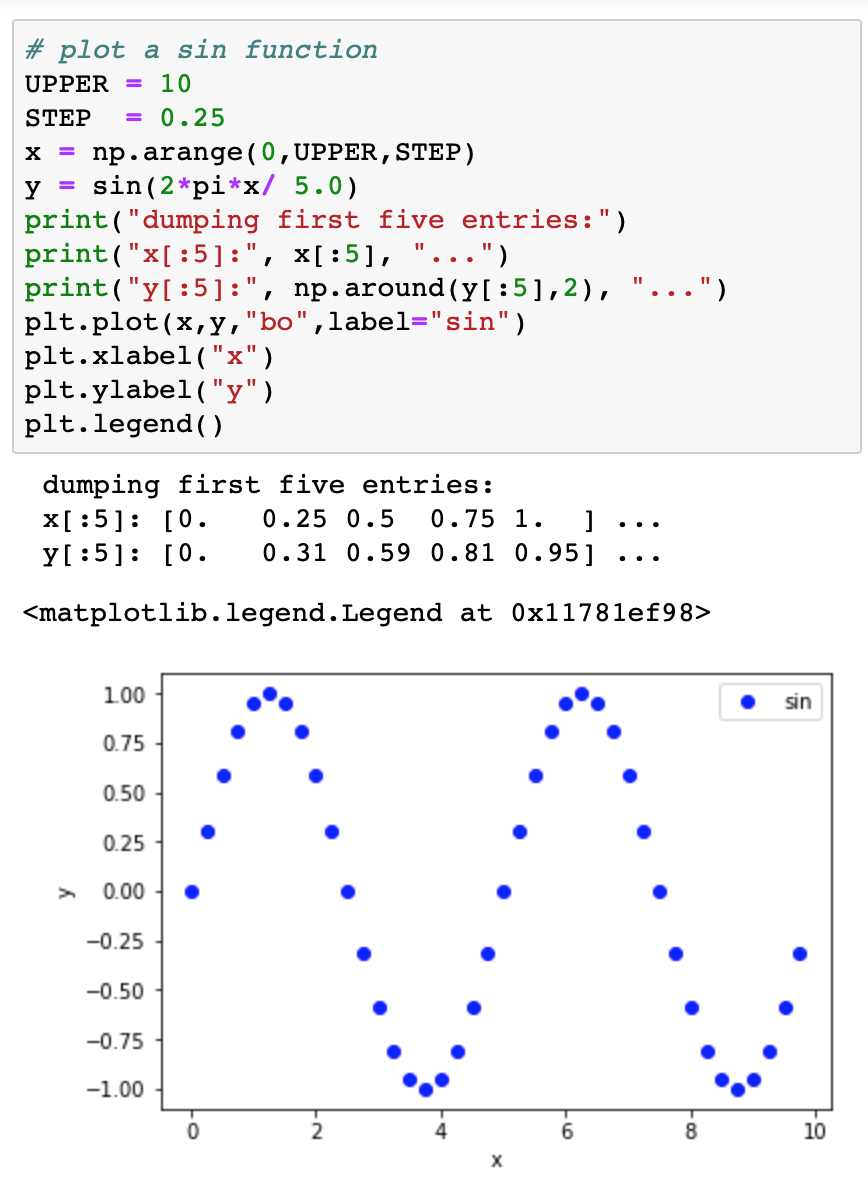
\includegraphics[width=0.65\textwidth]{figs//plotting/plotting.png} 
\caption{Circuit for verifying Ohm's law as a (a) circuit diagram, and (b) implemented using your lab equipment.}
\label{fig:plotsin}
\end{center}
\end{figure}

Consider the Jupyter notebook example in Fig.~\ref{fig:plotsin} which
plots a sine function sampled at discrete values.  Note the following
key features, which you will use repeatedly today and in future labs:
\begin{itemize}
\item Use of global variables {\tt UPPER} and {\tt STEP} at the top of
  the snippet, allowing for easy adjustment of parameters that affect
  the plot.
\item Use of {\tt np.arange} to define an array of x values.
\item Creation of the array y, defined by $y = \sin(2\pi x / 5)$ for each value of x.  One of the great joys of using numpy is the ability to avoid getting bogged down with explicit for loops.
\item Use of slicing techniques {\tt x[:5]} to show only the first five entries for debugging.  
\item Plotting the arrays of $x$ and $y$ values with {\tt plt.plot}  using the {\tt "bo"} option for blue circles.
\item Defining appropriate axis labels with {\tt plt.xlabel} and {\tt plt.xlabel}. 
\item Creation of a legend using the {\tt label} option to {\tt plt.plot} and the {plot.legend()} command.
\end{itemize}
Notice that even in this simple example, I've added some intermediate
feedback from my code in the form of the screen dumps of the first few
values of $x$ and $y$.  It's a common pitfall to try and rush ahead to
the final product when programming.  But it is much faster and
reliable to break your task into small steps, and establish feedback
at each small step.  To plot a continuous function with Scientific
Python, you will still use discrete data but:

\begin{itemize}
 \item Use much finer binning of the $x$-axis variable to draw a smooth curve. 
 \item Use the line option {\tt "-"} or dashed line {\tt "--"} instead of points with {\tt "o"}. 
\end{itemize} 

\noindent
{\bf Plot 1:}  Plot the quadratic function $y = x^2$ with the following requirements:
\begin{itemize}
 \item Plot in the range $x = [0,20)$.
 \item Plot discrete samples with a step size of $2$ using blue circles.
 \item On the same axis, plot the corresponding smooth function using a red solid line.
 \item Add appropriate axis labels. 
 \item Add a legend for the ``discrete'' and the ``smooth''  function.
\end{itemize}

\section{Multivariate analysis using boolean masks}
\begin{figure}[htbp]
\begin{center}
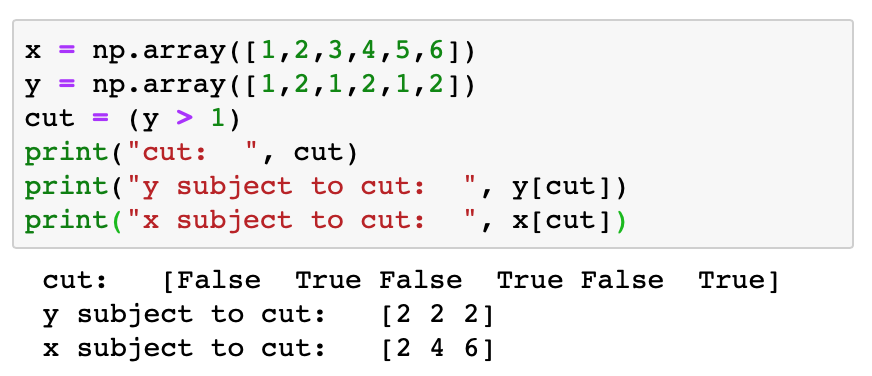
\includegraphics[width=0.65\textwidth]{figs//plotting/booleanmasks.png} 
\caption{Using boolean masks to cut on variable $y$.}
\label{fig:booleanmasks}
\end{center}
\end{figure}

A powerful technique in Scientific Python for performing analysis involving multiple variables uses boolean masks as shown in Fig.~\ref{fig:booleanmasks}.  In the example:
\begin{itemize}
\item Two numpy arrays $x$ and $y$ {\tt of the same length} are defined to contain the collected data.
\item The cut defined by $y > 1$ is a boolean array of the same length as $x$ and $y$ which is true at indices where the condition is met and false where it is not.
\item The subset of the entire $y$ array defined by {\tt y[cut]} consists only of those entries of $y$ for which the condition $y>1$ is met.
\item The subset of the entire $x$ array defined by {\tt x[cut]} consists only of those entries of $x$ for which the condition $y>1$ is met for the corresponding y value.
\end{itemize}
The last item shows the real power of this technique, one can look at one variable subject to constraints on another variable.

\begin{table}
\caption{Sample data for a voltage measurement subject to high frequency noise.}
\label{tbl:hfnoiseeg}
\begin{center}
\begin{tabular}{lll}
$t~(\rm s)$ & $v~(\rm V)$ & $n$ \\
0.4  & 0.25  &  2.8 \\
1.1  & 2.37  &  7.3 \\
1.4  & 1.69  &  9.7 \\
1.9  & 0.93  &  1.3 \\
2.5  & -1.0  &  6.2 \\
3.0  & 0.95  &  4.8 \\
3.4  & 1.22  &  6.9 \\
4.1  & 0.54  &  4.0 \\
4.4  & 0.37  &  1.9 \\
4.8  & 0.13  &  4.0 \\
5.5  & -2.04  &  9.5 \\
6.2  & -2.06  &  8.7 \\
6.5  & -0.81  &  2.3 \\
7.0  & -0.95  &  5.3 \\
7.5  & 0.98  &  9.7 \\
7.9  & 0.27  &  8.3 \\
8.5  & -0.81  &  0.1 \\
9.0  & -0.59  &  5.1 \\
9.4  & -0.37  &  4.4 \\
9.9  & 0.56  &  9.9 \\
\end{tabular}
\end{center}
\end{table}

Next consider the sample data in Table~\ref{tbl:hfnoiseeg} which comes from experimental measurements of a voltage level $v$ at discrete times $t$.  The measurement is subject to a high-frequency noise monitoring by the variable $n$.  The noise is only present for $n > 6.0$.  A straightforward way to load this data into scientific python is by defining numpy arrays for each variable as follows:
\begin{verbatim}
t = np.array([0.4, 1.1, 1.4, 1.9, 2.5, 3.0, 3.4, 4.1, 4.4, 4.8, 
                     5.5, 6.2, 6.5, 7.0, 7.5, 7.9, 8.5, 9.0, 9.4, 9.9])
v = np.array([ 0.25, 2.37, 1.69, 0.93, -1.0, 0.95, 1.22,   
                      0.54, 0.37, 0.13, -2.04, -2.06, -0.81, -0.95,  
                      0.98, 0.27, -0.81, -0.59, -0.37, 0.56])
n = np.array([2.8, 7.3, 9.7, 1.3, 6.2, 4.8, 6.9, 4.0, 1.9, 4.0,  
                      9.5, 8.7, 2.3, 5.3, 9.7, 8.3, 0.1, 5.1, 4.4, 9.9])
\end{verbatim}

\noindent
{\bf Plot 2} Prepare a plot of the sample data subject to the following:
\begin{itemize}
 \item Plot the voltage as a function of time as discrete data using red points.
 \item Define the boolean array {\tt keep} based on the noise reducing condition $n<=6.0$.
 \item Plot the voltage as a function of time, subject to the noise reducing condition using blue points.
 \item Plot the function $\sin(2 \pi x / 10)$ as a smooth function.
 \item Add appropriate axis labels.
 \item Add a legend for ``raw'' data with no cut, ``clean'' data with noise removed, and your continuous ``sin'' function.   
\end{itemize}
Your plot will reveal a clear sine function in the discrete data (after noise removal) consistent with the continuous function.  





\chapter{DC Circuits}

\section{Introduction}

In this lab, you will learn how to use your digital multimeter (DMM) and bench-top DC power supply to explore DC circuits involving resistors.  You will experimentally verify Ohm's law and the equivalent resistance for resistors in series and parallel.  You will solder two resistor circuits to explore the $\Delta$-$Y$ transformation for three terminal networks.

\section{Benchtop Power Supply}
% MASTECH HY3005F-3

\section{Digital Multimeter}
% Triplett 9007 (often blown fuse)
% Mastech MS8264 (resettable fuse)

\begin{figure}[htbp]
\begin{center}
\begin{tabular}{c@{\hskip 2cm}c}

\begin{circuitikz}[line width=1pt]
\draw (0,0) to[battery1,bipoles/length=1.5cm] ++(0,+4.0) to[short] ++(2.0,0) coordinate(A);
\draw (A) to[resistor,l_=$R_1$] ++(0,-2.0) to[short] ++(0,-2.0) to[short] ++(-2,0);
%node[ground,yscale=2.0]{};
\draw (0,1.7) node[left]{$-$};
\draw (0,2.4) node[left]{$+$};
\draw (A) to[short,*-] ++(2.0,0.0) to[short] ++(0.0,-1.0) node[component]{V} to[short] ++(0.0,-1.0) to[short,-*] ++(-2.0,0);
\end{circuitikz} &

\begin{circuitikz}[line width=1pt]
\draw (0,0) to[battery1,bipoles/length=1.5cm] ++(0,+4.0) to[short] ++(2.0,0);
\draw (A) to[resistor,l_=$R_1$] ++(0,-2.0) to[short] ++(0,-1.0) 
node[component]{A} to[short] ++(0,-1.0) to[short] ++(-2.0,0);
%node[ground,yscale=2.0]{};
\draw (0,1.7) node[left]{$-$};
\draw (0,2.4) node[left]{$+$};
\end{circuitikz} \\

(a) & (b) \\
\end{tabular}
\caption{Circuits for verifying Ohm's law.}
\label{fig:dmmscematic}
\end{center}
\end{figure}




% Triplett 9007 (often blown fuse)
% Mastech MS8264 (resettable fuse)
% Wish Board No.  206
% MASTECH HY3005F-3

In this lab, you will use two new pieces of lab equipment:  your bench-top power supply and your digital multimeter (DMM).

Your bench-top supply provides up to XX volts of DC power on two independent channels.  For this lab, we'll only be using a single channel.  Each supply has two associated knobs, one controlling the maximum allowed current, and one controlling the maximum voltage.  The supply will provide the maximum voltage subject to those constraints.  Usually your are primarily concerned with setting the voltage by the voltage knob, but it is a good habit, which will save you from losing components, to set the current as low as possible.  An LED indicates if your circuit is current limited or voltage limited.  You can adjust the current limit until just beyond the point where your circuit become voltage limited.

The supply is floating, it provides the specified voltage between the black and red outputs without referencing either to ground.  If you want to provide a ground referenced voltage you explicitly connect the green output to the red (positive) terminal or the black (negative) terminal.

(Discuss limits)

Your DMM can measure voltage, resistance, and current.






\section{Verification of Ohm's Law}

\begin{figure}[htbp]
\begin{center}
\begin{tabular}{c@{\hskip 2cm}c}

\begin{circuitikz}[line width=1pt]
\draw (0,0) to[battery1,bipoles/length=1.5cm] ++(0,+4.0) to[short] ++(2.0,0) coordinate(A);

\draw (A) to[resistor,l_=$R_1$] ++(0,-2.0) to[short] ++(0,-1.0) 
node[component]{A} to[short] ++(0,-1.0) to[short] ++(-2.0,0);
%node[ground,yscale=2.0]{};
\draw (0,1.7) node[left]{$-$};
\draw (0,2.4) node[left]{$+$};
\draw (A) to[short,*-] ++(2.0,0.0) to[short] ++(0.0,-1.0) node[component]{V} to[short] ++(0.0,-1.0) to[short,-*] ++(-2.0,0);
\end{circuitikz} &
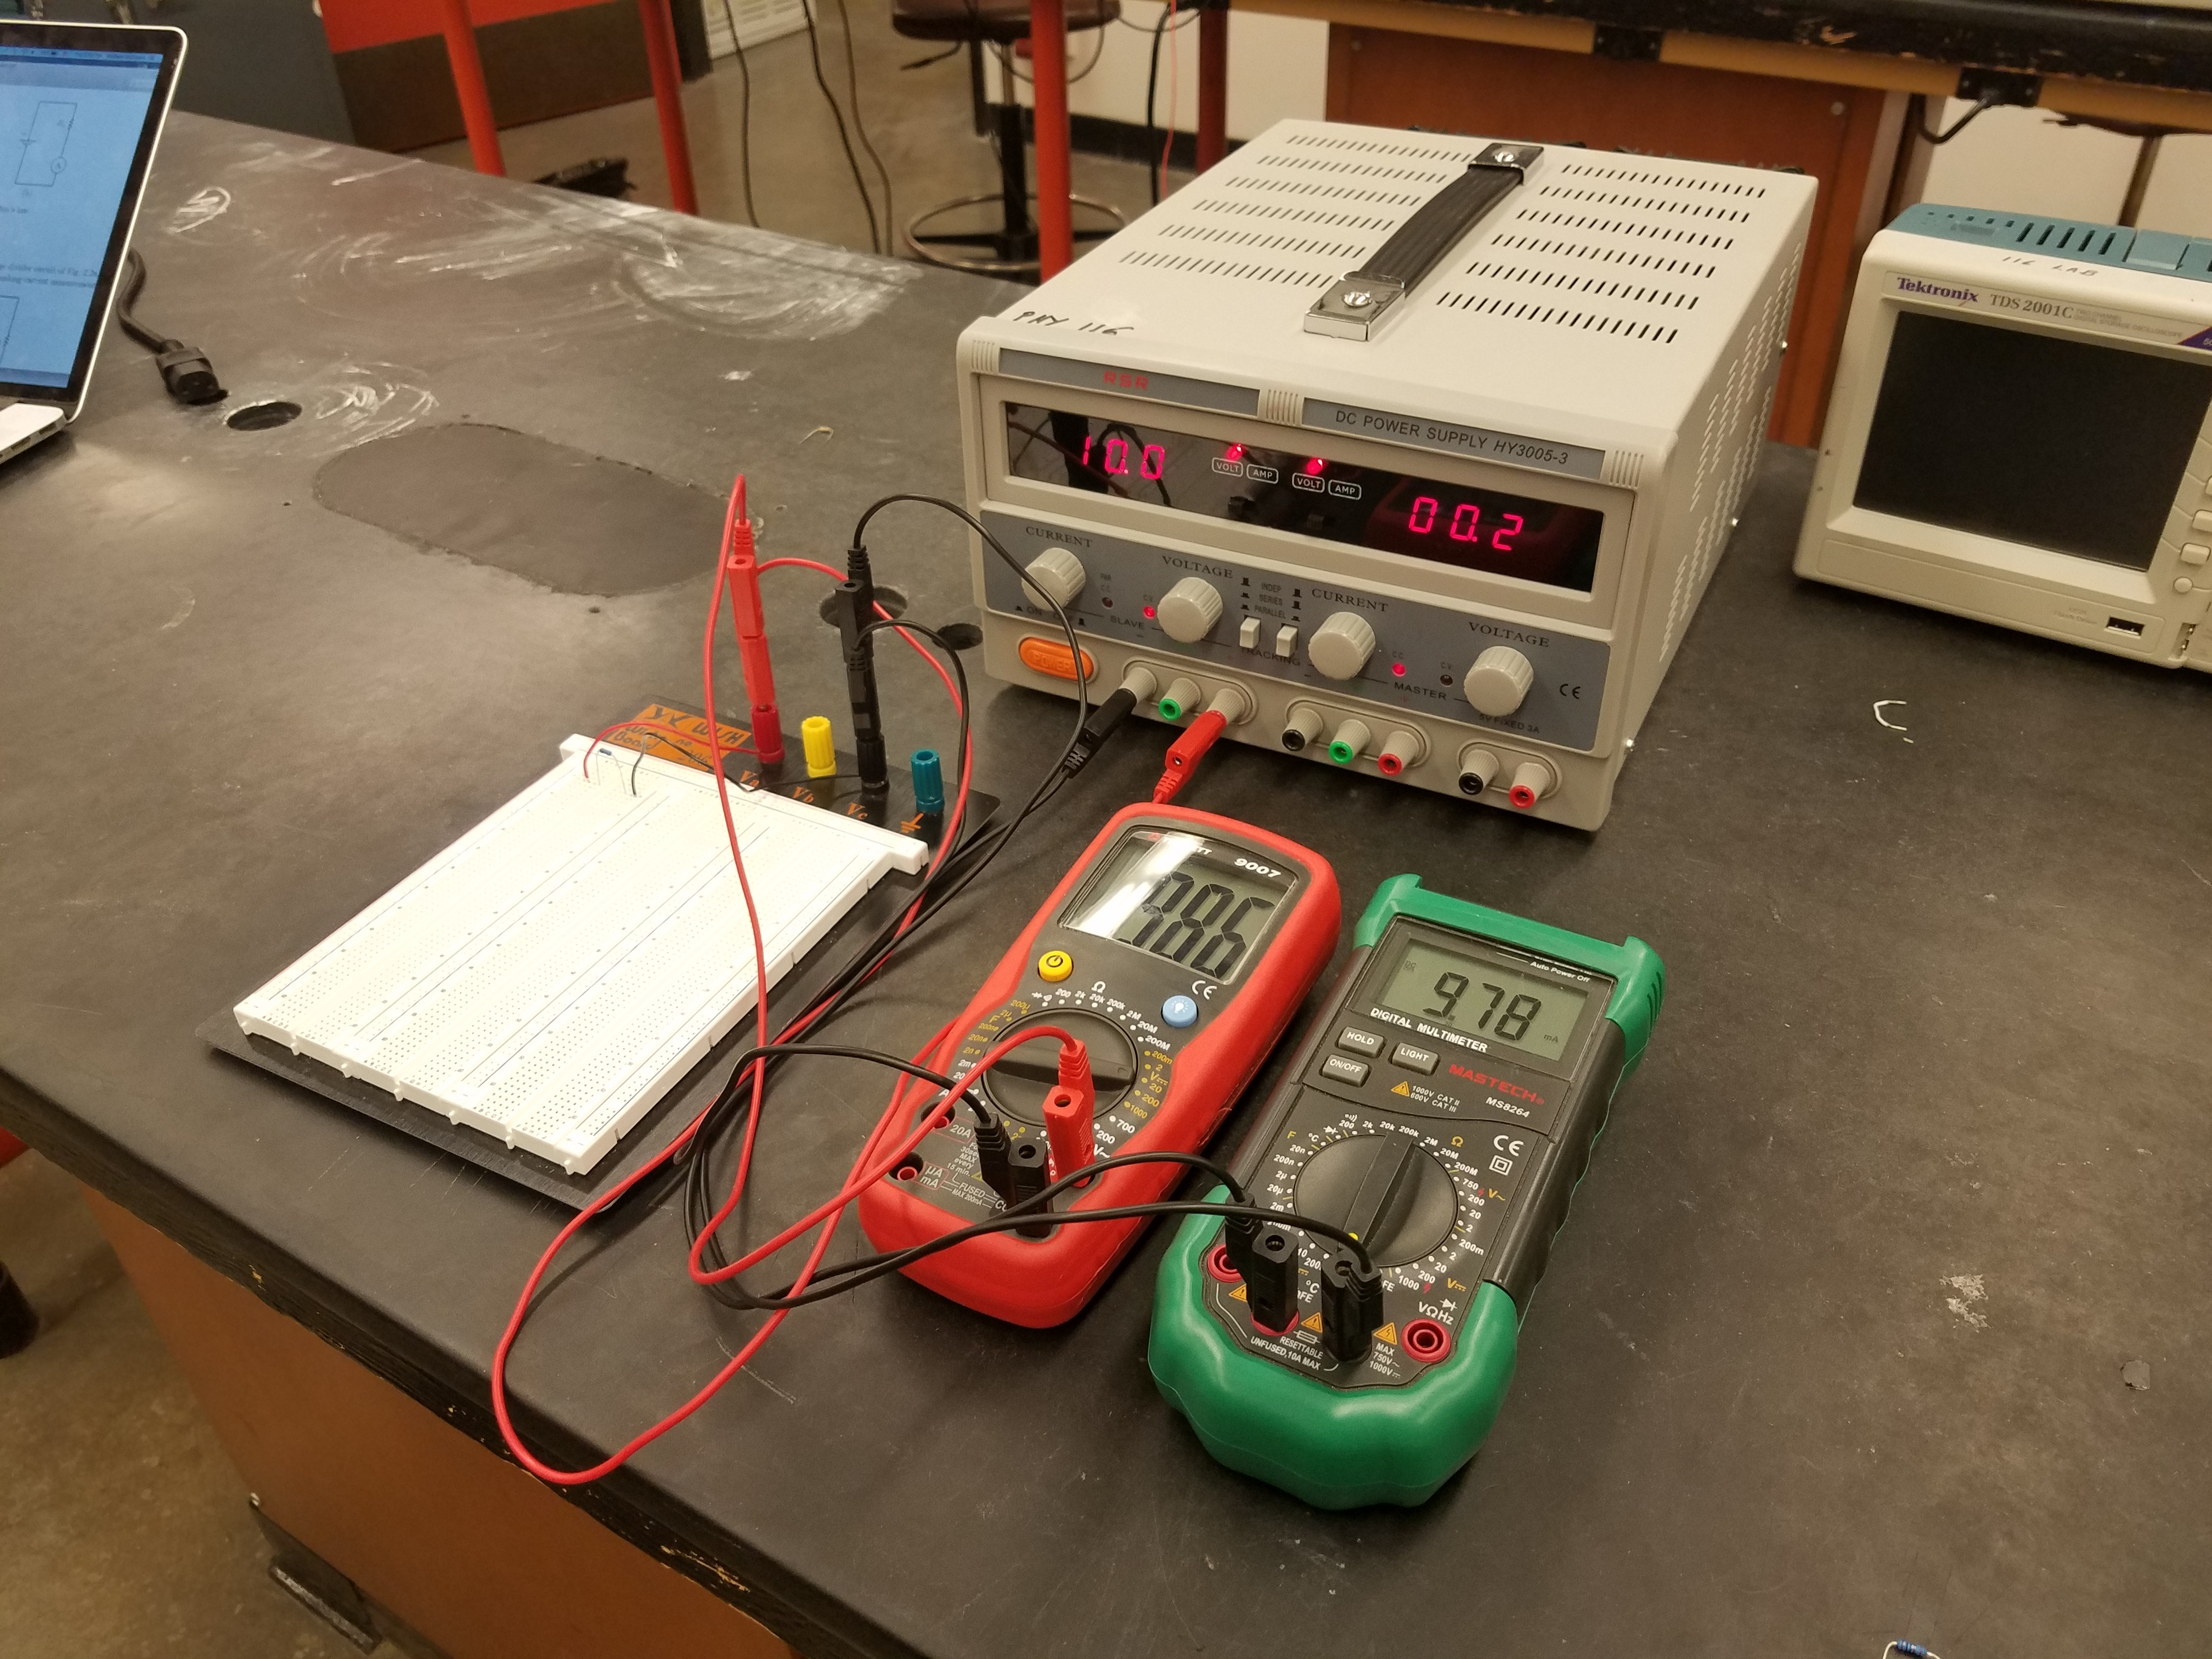
\includegraphics[height=0.25\textheight]{figs/labs/dc_circuits/setup.jpg} \\
(a) & (b) \\
\end{tabular}
\caption{Circuit for verifying Ohm's law as a (a) circuit diagram, and (b) implemented using your lab equipment.}
\label{fig:ohmslaw}
\end{center}
\end{figure}


Build the circuit in Fig.~\ref{fig:ohmslaw}.  Use a resistor $R_1 = 1.0~{\rm k\Omega}$ with a $1\%$ tolerance.  Use your Triplett 9007 as the voltmeter and the Mastech MS8624 as the current meter.  Use your benchtop power supply to provide the voltage.  

By adjusting the voltage setting of the power supply, take a series of voltage and current measurements with voltage across the resistor at target voltages from $1$ to $10~\rm V$ in steps of $1~\rm V$.   Generally, you can measure more precisely than you can control, so never fuss about trying to measure the voltage at exactly the target value, instead, simply record e.g. $V=1.04~\rm V$ along with your current measurement and move on to the next target value.

While recording data, check that the current values you measure are consistent with what you expect given the voltage across the resistor and resistance.  You should {\em always} make quick sanity calculations when collecting data, otherwise you risk wasting time collecting useless data!

{\bf Plot 1:}  Plot the current versus voltage of your ten data points (using option {\tt "o"}).  Draw a line (using option {\tt "-"}) for the current versus voltage curve of a $1.0~\rm k\Omega$ resistor.  Make certain your plot has appropriate axis labels, including appropriate units in parenthesis, and a legend distinguishing data from your expectation (``expected").  {\bf Measurement 1:}  After taking your last measurement, leave all the connections in place and the power-supply at $10~\rm V$.  Record in your log book the resistance of the resistor $R_1$ reported by your DMM.  Is this a reasonable measurement?  {\bf Measurement 2:}  Turn off the DC supply and record the resistance reported by the DMM.  Is this accurate?  {\bf Measurement 3:}  Remove the resistor from your circuit and measure the resistance with your DMM.  Is this accurate?

\begin{figure}[htbp]
\begin{center}
\begin{tabular}{c@{\hskip 2cm}c}

\begin{circuitikz}[line width=1pt]
\draw (0,0) to[battery1,bipoles/length=1.5cm] ++(0,+4.0) to[short] ++(2.0,0) coordinate(A);
\draw (A) to[resistor,l_=$R_1$] ++(0,-2.0) to[short] ++(0,-2.0) to[short] ++(-2,0);
%node[ground,yscale=2.0]{};
\draw (0,1.7) node[left]{$-$};
\draw (0,2.4) node[left]{$+$};
\draw (A) to[short,*-] ++(2.0,0.0) to[short] ++(0.0,-1.0) node[component]{V} to[short] ++(0.0,-1.0) to[short,-*] ++(-2.0,0);
\end{circuitikz} &

\begin{circuitikz}[line width=1pt]
\draw (0,0) to[battery1,bipoles/length=1.5cm] ++(0,+4.0) to[short] ++(2.0,0);
\draw (A) to[resistor,l_=$R_1$] ++(0,-2.0) to[short] ++(0,-1.0) 
node[component]{A} to[short] ++(0,-1.0) to[short] ++(-2.0,0);
%node[ground,yscale=2.0]{};
\draw (0,1.7) node[left]{$-$};
\draw (0,2.4) node[left]{$+$};
\end{circuitikz} \\
(a) & (b) \\
\end{tabular}
\caption{Circuits for verifying Ohm's law.}
\label{fig:missing}
\end{center}
\end{figure}


\section{Voltage Divider}
One circuit you will encounter again and again is the humble voltage divider circuit of Fig.~\ref{fig:dividers}a.  Modify your setup to include an additional resistor $R_2 = 4.7~\rm k\Omega$ in series with your resistor $R_1 = ~\rm 1~\rm k\Omega$.  Before installing it in your circuit, record the actual value of your resistor $R_2$ in your log book.

{\bf Measurement 4:} adjust the supply voltage to $10~\rm V$ and record the voltage across resistor $R_1$, the voltage across resistor $R_2$, and the current through the divider.  Compare these measured values to your expectation.

Now adjust your circuit so that $R_1$ and $R_2$ are in parallel and set the supply to $10~\rm V$  {\bf Measurement 5:}  Record the voltage across the resistors $R_1$ and $R_2$ and the total current through both resistors.  Compare the measured current to your expectation.

\begin{figure}[htbp]
\begin{center}
\begin{tabular}{c@{\hskip 2cm}c}
\begin{circuitikz}[line width=1pt]
\draw (0,0) to[battery1,bipoles/length=1.5cm] ++(0,+4.0) to[short] ++(2.0,0);
\draw (A) to[resistor,l_=$R_1$] ++(0,-2.0) to[resistor,l_=$R_2$] ++(0,-2.0) to[short] ++(-2.0,0);
%node[ground,yscale=2.0]{};
\draw (0,1.7) node[left]{$-$};
\draw (0,2.4) node[left]{$+$};
\end{circuitikz} &
\begin{circuitikz}[line width=1pt]
\draw (0,0) to[battery1,bipoles/length=1.5cm] ++(0,+4.0) to[short] ++(2.0,0) coordinate(A);
\draw (A) to[resistor,l_=$R_1$] ++(0,-4.0) to[short] ++(-2,0);
%node[ground,yscale=2.0]{};
\draw (0,1.7) node[left]{$-$};
\draw (0,2.4) node[left]{$+$};
\draw (A) to[short,*-] ++(2.0,0.0) to[resistor,l_=$R_2$] ++(0.0,-4.0) to[short,-*] ++(-2.0,0);
\end{circuitikz} \\
(a) & (b) \\
\end{tabular}
\caption{Circuits for driving an LED (a) directly from the signal voltage and (b) using a diode switch.}
\label{fig:dividers}
\end{center}
\end{figure}


\section{$\Delta$-$Y$ transformation}

Consider the two different circuits shown in Fig.~\ref{fig:deltay}.  If we are willing to neglect the central vertex in the left hand circuit, the two circuits are equivalent in the case that $R_1 = R_2 / 3$.   Using your soldering iron, 




\begin{figure}[htbp]
\begin{center}
\begin{tabular}{c@{\hskip 2cm}c}
\begin{circuitikz}[line width=1pt]
\draw (0,0) coordinate(A);
\draw (A) to[R,l_=$R_1$,*-*] ++(0,2.0);
\draw (A) to[R,*-*] ++(-1.73,-1);
\draw (A) to[R,*-*] ++(1.73,-1);
\draw (-0.5,0) node[left]{$R_1$};
\draw (1.25,0) node[left]{$R_1$};

\end{circuitikz} &
\begin{circuitikz}[line width=1pt]
\draw (0,2) to [R] (1.73,-1) to [R,*-,l_=$R_2$] (-1.73,-1) to [R,*-*] (0,2);
\end{circuitikz} \\
(a) & (b) \\
\end{tabular}
\caption{Equivalent three-node circuits.}
\label{fig:deltay}
\end{center}
\end{figure}


\section{Additions}

Effect of resistance measurement with current in resistor?

Loading of circuit by DMM.



\chapter{Equivalent Circuits}

In this lab, you will explore Thevenin equivalent circuits. You will
also solder two resistor circuits to explore the $\Delta$-$Y$
transformation for three terminal networks. For this lab, both logbook
and Jupyter Notebook entries are required. You can find the resistors
inside storage cabinet at the table to your left and cables hanging at
the wall to your left. Please return them at the end of the lab.

\section{Calculations}

\noindent
During lecture we determined an equation for the Thevenin
equivalent voltage $V_{\rm th}$ and resistance $R_{\rm th}$ from the
values $V_1, V_2, R_1, R_2, R_3$ for the circuit shown in
Fig.~\ref{fig:thevenin}.
%Hint: Use the superposition principle. Find the equivalent resistance
%by setting the voltage $V_1$ and $V_2$ to zero, i.e. shorting them in
%the circuit.  Then calculate two contributions to the Thevenin
%voltage, one with $V_1$ set to zero and one with $V_2$ set to zero.
%The actual Thevenin voltage is the sum of these two contributions.
%Play close attention to the polarity of $V_2$ as drawn, i.e. that a
%positive value of $V_2$ tends to make the voltage $V_{\rm a b}$
%negative.

\begin{measurement} 
Repeat this calculation in terms of $V_1, V_2, R_1, R_2, R_3$ in your
logbook together with the sketch of the circuit.
\end{measurement}

\begin{figure}[htbp]
\begin{center}
\begin{tabular}{c@{\hskip 2cm}c}
\begin{circuitikz}[line width=1pt]
\draw (0,0) to[voltage source,bipoles/length=1.5cm,l=$V_1$,invert] ++(0,2.0)
coordinate(X) to[R,l=$R_3$,-*] ++(2.0,0); \draw (X) to[R,l=$R_1$]
++(0,2.0) to[short,-*] ++ (2.0,0) coordinate(X) to[short,-o] ++
(1.0,0) node[right]{B}; \draw (X) to[voltage
  source,bipoles/length=1.5cm, l=$V_2$,invert] ++(0,-2.0) to[R,l=$R_2$]
++(0,-2.0) coordinate(X) to[short,*-o] ++ (1.0,0) node[right]{A};
\draw(X) to[short] ++(-2.0,0);
\end{circuitikz} &
\begin{circuitikz}[line width=1pt]
\draw (0,0) coordinate(X) to[voltage source,bipoles/length=1.5cm,l=$V_{\rm th}$,invert] ++(0,2.0) to[R,l=$R_{\rm th}$,-*] ++(0,2.0)
to[short,-o] ++ (3.0,0) node[right]{B};
\draw(X) to[short,-o] ++ (3.0,0) node[right]{A};
\end{circuitikz} \\
(a) & (b) \\
\end{tabular}
\caption{The circuit (a) you will be building in lab and it's (b) Thevenin Equilvalent.}
\label{fig:thevenin}
\end{center}
\end{figure}

\section{Thevenin Equivalent Circuit}

Build the circuit (on a breadboard) in Fig.~\ref{fig:thevenin} using $R_1 = 3.3~\rm
k\Omega$, $R_2 = 3.9~\rm k\Omega$, and $R_3 = 4.7~\rm k\Omega$.
Supply $V_1 = 10~\rm V$ and $V_2 = 5~\rm V$ using your two channel
bench-top power supply.  In the diagram, the supplies are not
referenced to ground or each other, so make certain that your supply
is set to provide independent outputs and do not add any jumpers to
ground.  Take careful note of the polarity of the supplies, so
e.g. the negative (black) output of $V_1$ is connected to point (A)
whereas the negative (black) output of $V_2$ is connected to point
(B).Use your Triplett 9007 as a voltmeter and the Mastech MS8624 as a
current meter.   

\begin{measurement} 
Compute $V_{\rm th}$, $R_{\rm th}$, and the short-circuit current
$I_{\rm sc}$ for the particular values of $R_1$,$R_2$,$R_3$,$V_1$, and
$V_2$ you will be using in the lab. Record these values in your logbook.  
\end{measurement}

\begin{measurement} 
First measure the open circuit voltage $V_{\rm ab}$.  Next short the
points (a) and (b) through your current meter. Record these values in
your logbook.  These values should closely match the Thevenin voltage
and short-circuit current which you have already calculated.  If not,
you should check your work and find the discrepancy before
proceeding. Record your comments in the logbook.
\end{measurement}

\begin{measurement}  
Next you will measure the voltage across and current through a load
resistor connected between the terminals at (A) and (B) to
experimentally determine the IV curve for your circuit.  Recall from
the previous lab that you measure the current by connecting your meter
in series and the voltage by connecting your meter in parallel.  As
before, use your Triplett 9007 as a voltmeter and the Mastech MS8624
as a current meter. Make simultaneous current and voltage measurements
for three different values of the load resistance $R = 470~{\rm
  \Omega}, 1.2~\rm k\Omega, 4.7~\rm k\Omega.$ Record these values in
your logbook.
\end{measurement}

\section{Analysis}

\begin{plot}
To present your analysis you should produce a plot similar to that of
Fig.~\ref{fig:egthev}.  Your plot should show the Thevenin equivalent
source IV curve for the circuit you built in lab.  You should also
draw theoretical load IV curves for the three resistor values you used
to make current and voltage.  Finally, you should include data points
for the five current and voltage measurements which you have made.
\end{plot}

\begin{figure}[htbp]
\begin{center}
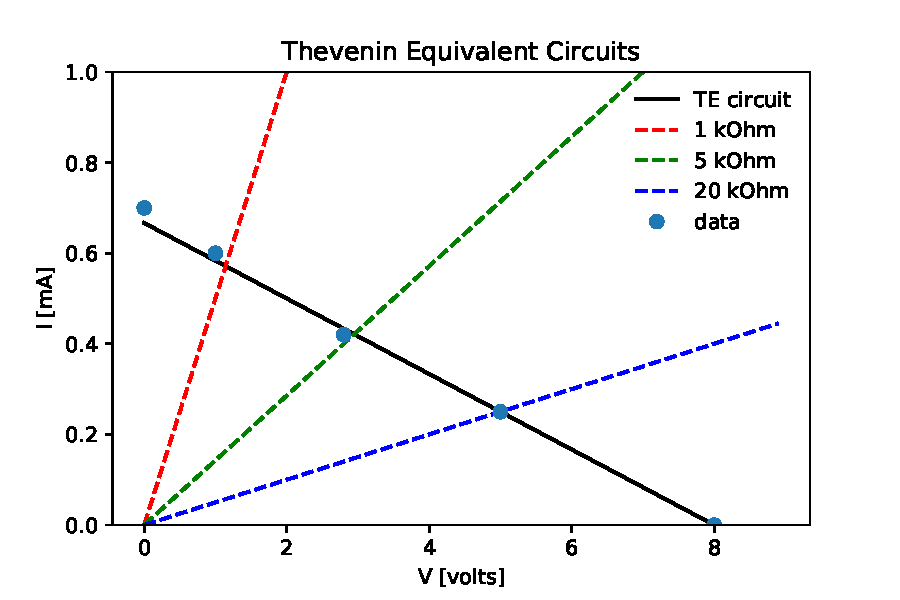
\includegraphics[width=0.75\textwidth]{figs/labs/thevenin/final.pdf} 
\caption{Example of IV curves for Thevenin equivalent source circuit with various load resistors. }
\label{fig:egthev}
\end{center}
\end{figure}

\section{Impact of the Multimeter on the Measured Circuit}

A perfect DMM would not affect the circuit you are measuring at all,
but this is not the case in practice. An ideal voltmeter has infinite
resistance so that it draws zero current when measuring voltage across
two points. An ideal ammeter has zero resistance so that there is no
voltage change as the current passes through it.  Your DMM has a small
non-zero resistance when used as an ammeter, and a large resistance
when used as a voltmeter.

\begin{measurement} 
Build the voltage divider of Fig.~\ref{fig:dividers}a but with
$V_1=10~\rm{V}$ and $R_1 = R_2 = 10~\rm{M\Omega}$. Record the voltage
across one of the resistors. Compare the value your measure with what
you predict for a perfect DMM. Sketch the circuit with a realistic DMM
and calculate the resistance of your DMM when used as a voltmeter.
\end{measurement}

\noindent
This is a \textbf{sign-off point} for this lab. 

\section{$\Delta-Y$ Transformation}

Not everyone will complete this portion of the lab.  Do your best to
finish as much as you can.

\begin{figure}[htbp]
\begin{center}
\begin{tabular}{c@{\hskip 2cm}c}
\begin{circuitikz}[line width=1pt]
\draw (0,0) coordinate(A);
\draw (A) to[R,l_=$R_A$,*-*] ++(0,2.0) node[above]{A};
\draw (A) to[R,*-*] ++(-1.73,-1) node[left]{B};
\draw (A) to[R,*-*] ++(1.73,-1) node[right]{C};
\draw (-0.5,0) node[left]{$R_B$};
\draw (1.25,0) node[left]{$R_C$};

\end{circuitikz} &
\begin{circuitikz}[line width=1pt]
\draw (0,2) to [R] (1.73,-1) node[right]{C} to [R,*-,l_=$R_{BC}$] (-1.73,-1) node[left]{B} to [R,*-*] (0,2) node[above]{A};
\draw (-0.75,1) node[left]{$R_{AB}$};
\draw (0.8,1) node[right]{$R_{AC}$};
\end{circuitikz} \\
(a) & (b) \\
\end{tabular}
\caption{Equivalent three-node circuits.}
\label{fig:deltay}
\end{center}
\end{figure}

Consider the two different networks shown in Fig.~\ref{fig:deltay}.
If there are no external connections to the central node in the
left-hand circuit, the two networks are equivalent if:
\begin{displaymath}
R_{A} = \frac{R_{AC} R_{AB}}{R_{AB} + R_{AC} + R_{BC}}
\end{displaymath}
as well as two similar equations for $R_{B}$ and $R_{C}$.  Going in the other direction we have:
\begin{displaymath}
R_{AB} = \frac{R_{A}R_{B} + R_{A}R_{C} + R_{B}R_{C}}{R_{C}}.
\end{displaymath}
These transformations are more general than the series and parallel
laws, which you can derive by considering the case that $R_{BC}=0$ for
parallel resistors, and $R_{C} \to \infty$ for series resistors.  They
allow one to simplify more complicated networks for which the series and
parallel equivalence relations are insufficient.

In the special case that $R_{A} = R_{B} = R_{C} = R$ it follows that 
\begin{displaymath}
R_{AB} = R_{AC} = R_{BC} = 3 R.
\end{displaymath}

Use your soldering iron to construct the left-hand network using
$R_{A} = R_{B} = R_{C} = 1~\rm k\Omega$.  Then construct the
equivalent right-hand network using $R_{AB} = R_{AC} = R_{BC} =
3.0~\rm k\Omega$.  If $3~\rm k\Omega$ resistors are not available, you
can construct one by using a $33~\rm k\Omega$ in parallel with a
$3.3~\rm k\Omega$ resistor.

Make sure the soldering iron is on, and the sponge is moist.  There is
one soldering iron per two workstation. Find the squeeze bottle around
the lab. The clamps (possibly various styles) are on the shelves to
your left. Twist the leads of the resistor together to make initial
connections, then hold the arrangement securely in the clamp.  Wipe
the tip of the hot iron on the sponge to clean it, then apply a small
amount of solder to the tip by touching the hot iron to the solder
wire.

Heat the connection by holding the soldering iron against it, then
bring the solder wire in contact with the heated connection (not the
soldering iron) You want the iron to heat the connection, and then the
connection to melt and draw in the solder.  The little bit of solder
on the tip is only there to ensure good thermal conduct between the
tip and the connection: don't ``paint'' the solder onto the
connection.

\begin{measurement} 
Check the resistance between pairs of terminals on your creations, and
compare with your expectation. Record those values in your logbook. You can bring your creations home if
you like or bring them to the front desk. 
\end{measurement}

This is an additional \textbf{sign-off point} for this lab. 

\noindent
Please return all the components you took and cables to their place. Leave you workstation clean. 


\chapter{Alternating Current and Time Varying Signals}

\section{Introduction}

In this lab you will use two essential new pieces of lab equipment:
the digital oscilloscope and the function generator.  You will learn
how to measure AC voltages with your DMM, how to trigger on and view
time-dependent wave forms on your digital oscilloscope.  You will
produce Lissajous figures on your oscilloscope and reproduce them
using Scientific Python.  For this lab there are both logbook and
Jupyter notebook entries.

\section{Function Generator}

This section introduces you to your Function Generator and illustrates
some of the common used features and pitfalls.  It should not take
more than about one-half hour to complete.

Connect the output of Channel 1 directly to the Voltage measurement
input of your Triplett 9007 DMM, using a coaxial cable with BNC
connectors, and a BNC to banana plug adapter as shown in
Fig.~\ref{fig:dmm_setup}.  BNC is a type of quick connector often used
for coaxial cable.  Coaxial cable is a type of electrical cable that
can transmit high frequency signals with low losses. It has an inner
conductor surrounded by an insulating layer, surrounded by a
conducting shield.  Coaxial cable has a characteristic impedance,
which specifies the resistance that should be placed at the receiving
end of the cable to minimize reflections, which can degrade high
frequency signals.  Your coaxial cable has a characteristic impedance
of $50~\rm \Omega$.

\begin{figure}[htbp]
\begin{center}
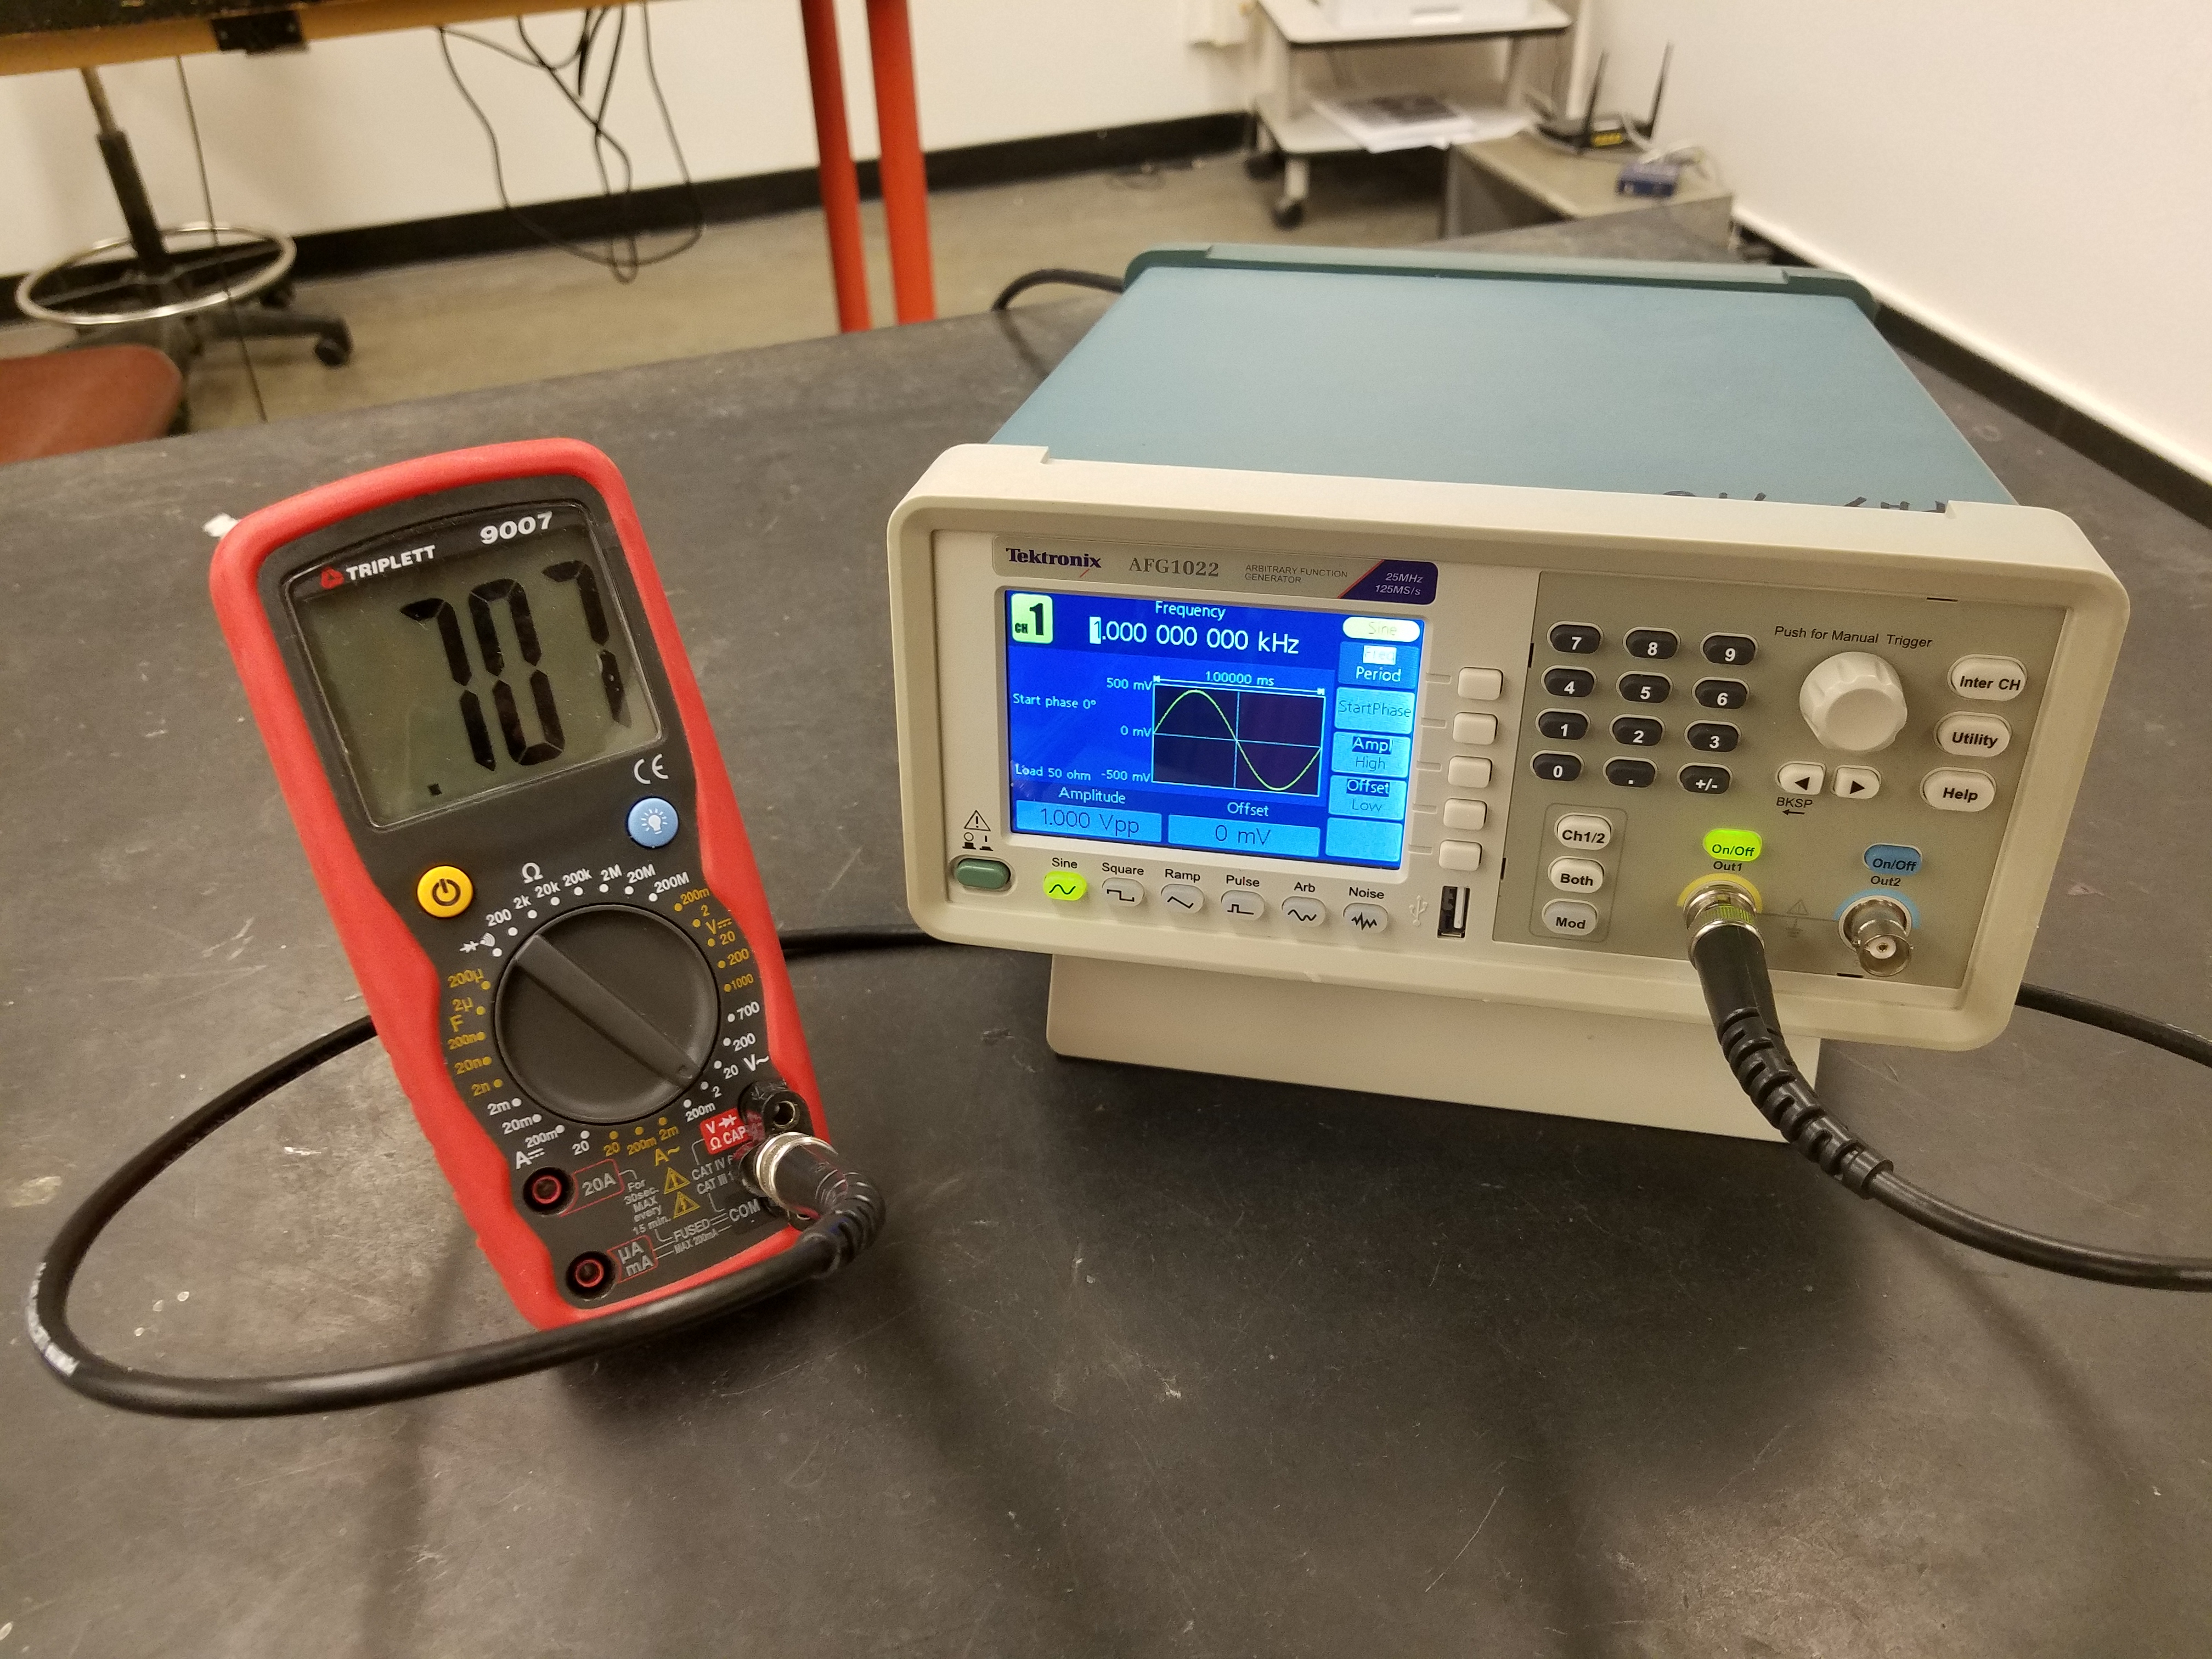
\includegraphics[width=0.45\textwidth]{figs/labs/lissajous/generator_dmm_setup.jpg} 
\caption{Connect the Channel 1 Output of your function generator directly to your DMM.}
\label{fig:dmm_setup}
\end{center}
\end{figure}

Turn on power to the function generator.  Then set your function
generator to the factory default:
\begin{displaymath}
\rm Utility\;Button \to System \to Set\;to\;Default \to Select.
\end{displaymath}
You must perform this step today for the instructions that follow to
make sense.  With shared equipment, it is essential to know how to
restore the factory default, in case another user has left the device
with strange settings.  You don't need to start with this step every
lab, but it is a fast way to recover when you encounter strange
behavior in your equipment.

The factory default settings are set to produce a Sine function with a
peak-to-peak voltage $v_{\rm pp} = 1.0~\rm V$ and a frequency $f=1~\rm
kHz$.  We'll leave that as is for now.  To turn on the output, push
the ``On/Off'' directly above the coaxial output for Channel 1, and
then ensure that the button is lit.

\begin{figure}[htbp]
\begin{center}
\begin{tabular}{ccc}
\begin{circuitikz}[line width=1pt]
\draw (0,0) coordinate(X) to[sinusoidal voltage source,bipoles/length=1.5cm] ++(0,2.0) 
to[R,l=$R_{\rm S}$] ++(0,2.0) to[short,-o] ++(1.0, 0) node[right]{B};
\draw (0.2,3.0) node[right] {$50~\rm \Omega$};
\draw (X) node[ground,yscale=2.0]{} to[short,-o] ++(1.0,0) node[right]{A};
\draw (0,-0.5) node[]{};
\end{circuitikz} &
\begin{circuitikz}[line width=1pt]
\draw (0,0) coordinate(X) to[short] ++(0,2.0) node[component]{V} to[short] ++(0,2.0) to[short,-o] ++(-1.0, 0) node[left]{B};
\draw (X) to[short,-o] ++(-1.0,0) node[left]{A};
\draw (0,-0.5) node[]{};
\end{circuitikz} &
\begin{circuitikz}[line width=1pt]
\draw (0,0) coordinate(X) to[short] ++(0,2.0) node[component]{V} to[short] ++(0,2.0) to[short] ++(-1.0, 0);
\draw (X) to[short,-*] ++(-1.0,0) coordinate(X) to[R,l=$R_L$] ++(0,4.0) to[short,*-o] ++(-1.0,0) node[left]{B};
\draw (X) to[short,-o] ++(-1.0,0) node[left]{A};
\draw (0,-0.5) node[]{};
\end{circuitikz} \\
(a) & (b) & (c) \\
\end{tabular}
\caption{Equivalent circuit for (a) your function generator, which includes a $50~\rm \Omega$ source resistance, and two typical terminations for a coaxial signal:  (b) infinite resistance voltmeter or scope, or (c) a terminating resistor in parallel.}
\label{fig:funccirc}
\end{center}
\end{figure}

\begin{measurement} Set your DMM to the $2~\rm V$ (AC) scale (the V with a squiggly line).  Measure the AC voltage, which should be close to: 
\begin{displaymath}
v_{\rm rms} = 0.707~\rm V \sim \frac{1}{\sqrt{2}}~\rm V
\end{displaymath} 
Record the measured value in your logbook with a sketch of
your circuit.
\end{measurement}
However, recalling the relationships between the peak-to-peak voltage,
the peak-voltage, and the RMS voltage of an AC sine wave:
\begin{displaymath}
v_{\rm pp} = 2 \, v_{\rm p} = 2 \sqrt{2} \, v_{\rm rms}
\end{displaymath}
we expect our function generator, set to $v_{\rm pp} = 1.0$, to
produce output with:
\begin{displaymath}
v_{\rm rms} = \frac{v_{\rm pp}}{2\sqrt{2}} \sim 0.353~\rm V
\end{displaymath}
Clearly someone is lying to us!  In fact, we've encountered a very
common source of factor of two mistakes.  The equivalent circuit for
your function generator is shown in Fig.~\ref{fig:funccirc}a.  Notice
that it includes a $50~\rm \Omega$ source resistance in series with
the AC voltage produced by the function generator.  This internal
resistance is important for a number of reasons, most notably making
it impossible to short-circuit the output and destroy the
equipment!

In our setup, we've connected the function generator output directly
to your DMM, which has a very high input resistance, effectively
infinite, as shown in Fig.~\ref{fig:funccirc}b.  However, the standard
termination for coaxial cables is $50~\rm \Omega$, and the default
setting for your function generator expects the load shown in
Fig.~\ref{fig:funccirc}c with $R_{\rm L} = 50~\rm \Omega$.  In
this case, the internal resistance and load resistance form a voltage
divider, so that the output voltage $V_{\rm AB}$ seen by the user is
$1/2$ the internal AC voltage. The function generator is designed to
produce an internal AC voltage which is twice the value selected by
the user, so that the output voltage is precisely the value specified
by the user.  We are seeing twice our requested value, because we have
no load resistor, and so no voltage divider, and instead see the full
value of internal AC voltage.  
\begin{measurement} To fix this discrepancy, we simply have
to configure our generator to expect a high load resistance at both
outputs:
\begin{eqnarray*}
{\rm Utility~Button \to Output Setup \to CH1Load \to HighZ} \\
{\rm CH2Load \to HighZ}
\end{eqnarray*}
Press the ``Ch1/2'' button until you return to the Channel 1 menu.  Adjust the amplitude to $1~{\rm V}$ peak-to-peak by:
\begin{displaymath}
\rm Ampl \to 1 \to Vpp
\end{displaymath}
Your DMM should now read the expected value:
\begin{displaymath}
v_{\rm rms} \sim 0.353~\rm V
\end{displaymath}
Record the measured value in your logbook, and explain, in your own words, why this differs from the previous measurement.
\end{measurement}

Press the button next to Ampl a couple of times.  There is a slightly
annoying feature of your function generator which allows you to
specify either the Amplitude and Offset or the High and Low voltage
values.  So if you want to adjust the Amplitude, you have to press the
button next to Ampl until the Ampl label is highlighted.  Often you'll
end up setting the wrong value by mistake.  But in general, whatever
parameter is highlighted along the side of the screen is the parameter
which you can specify by either the knob or the key pad.  
\begin{measurement} Keeping this
is mind, set your function generator to produce $1~\rm V$ RMS output:
\begin{displaymath}
\rm Ampl \to 1 \to Vrms.
\end{displaymath}
Now your DMM should also read a value quite close to one. Record this
value and instrumental uncertainty in your logbook.
\end{measurement}

\begin{measurement}
Now let's adjust the frequency. Highlight the frequency parameter by
pressing the button next to the ``Freq'' option until it is
highlighted:
\begin{displaymath}
\rm Freq \to 10 \to kHz.
\end{displaymath}
You can also adjust the selected parameter with the multipurpose knob.
Turn the multipurpose knob until the frequency is around $100~\rm kHz$
and observe what happens to your DMM measurement.  Record your
observation in your logbook. The reason your measurement is now
inconsistent with the setting in the function generator, is that your
DMM is only rated to $2~\rm kHz$.  It isn't intended for measuring
high-frequency AC signals.  Turn the frequency back down to $1~\rm
kHz$.
\end{measurement}

\begin{measurement}
Next highlight the Offset parameter on your function generator and
adjust it to $2~\rm V$.  This will add a DC offset to your function
generator output.  After settling down, the measured value of the AC
voltage on your DMM should be unchanged at $1~\rm V$.  Switch your DMM
to measure the DC voltage and you should now measure the $2~\rm V$ DC
offset.  Record the measured AC and DC voltages that you have measured
and sketch the waveform ($V(t)$) for one period, which is $1~\rm ms$
for this $1~\rm kHz$ signal.

Pay attention to the sign.  If you see a negative value, it is because
you installed your BNC-to-banana adapter incorrectly.  Notice that one
side of the adapter has a small raised tab, indicating which side
connects to the coaxial cable shield.  The side with the raised tab
should be plugged into the Common socket.  Whether you got lucky this
time or not, change the orientation of the adapter a few times and
observe how the sign of the voltage changes, finally plugging it back
in with the correct orientation. Now adjust the DC level with the
multipurpose knob and observe the change on your DMM.  When satisfied,
set the offset back to zero. 
\end{measurement}

\section{Oscilloscope}

This section introduces you to your Oscilloscope.  It should not take
more than about one-half hour to complete.

\begin{figure}[htbp]
\begin{center}
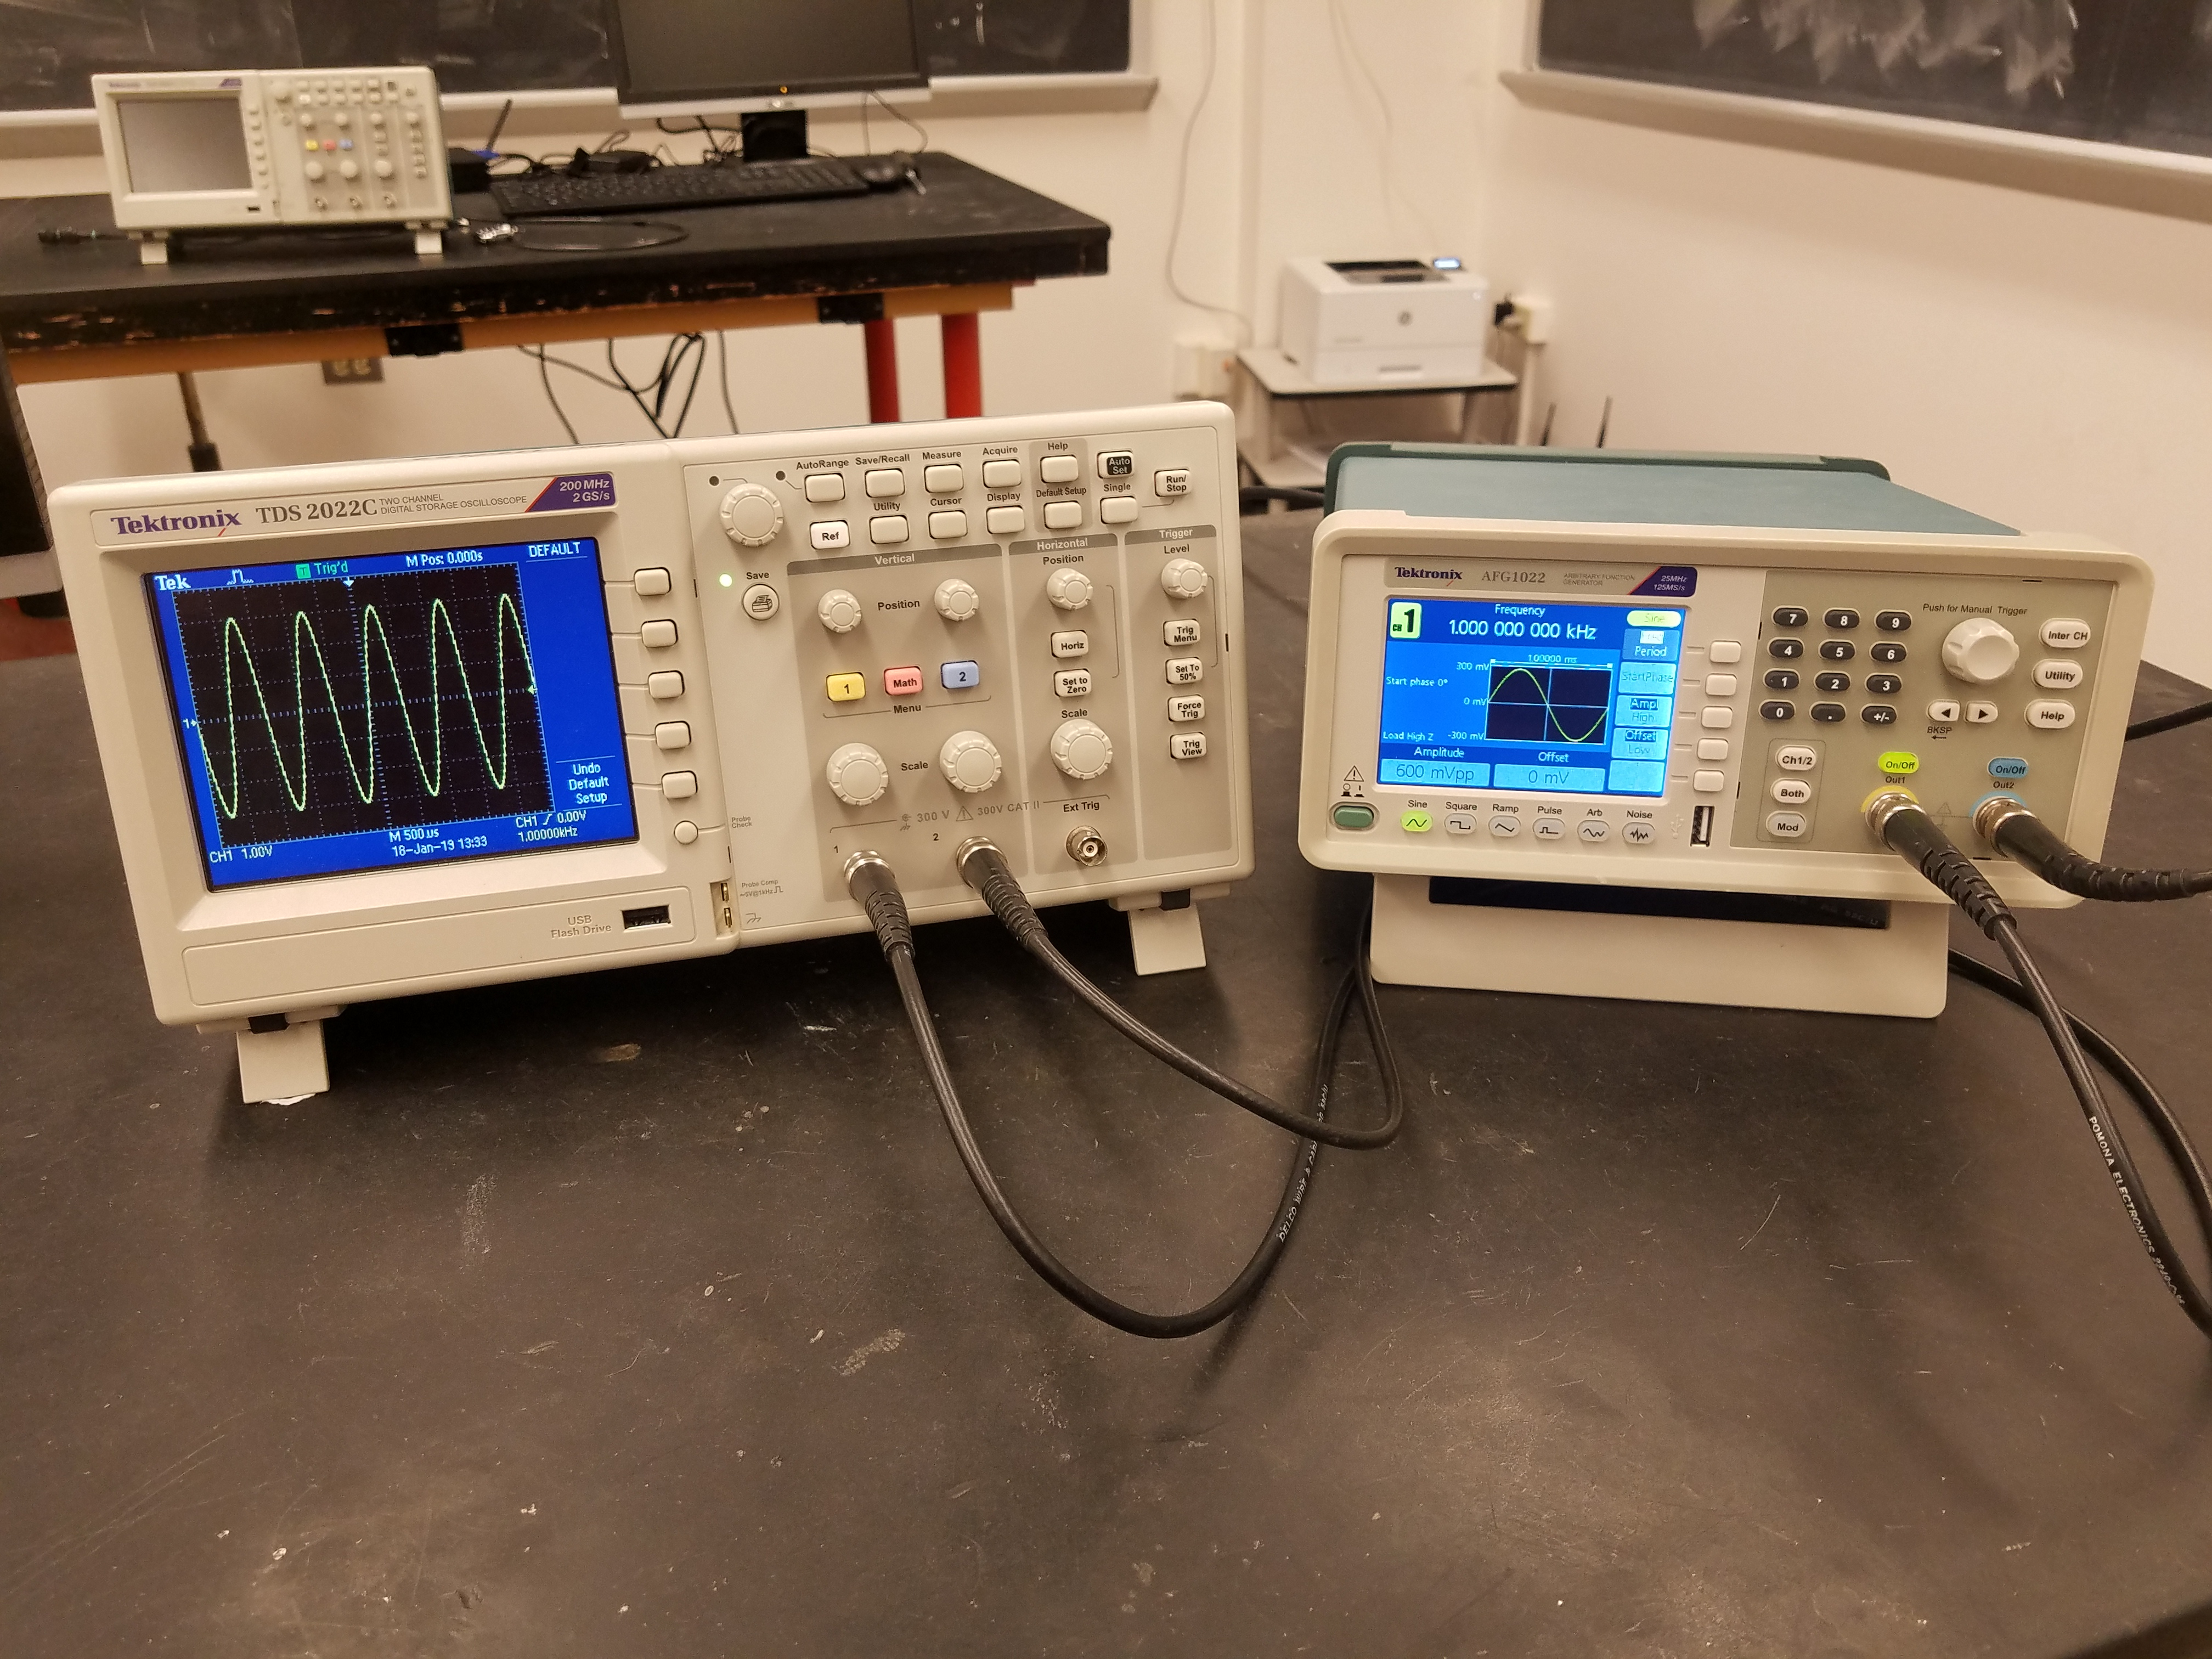
\includegraphics[width=0.45\textwidth]{figs/labs/lissajous/scope_setup.jpg} 
\caption{Connect the Channel 1 Output of your function generator directly to the Channel 1 input of your digital oscilloscope.}
\label{fig:scope_setup}
\end{center}
\end{figure}

Put your DMM aside.  Connect the Channel 1 output of your function
generator to the Channel 1 input of your digital oscilloscope.  Do the
same for Channel 2.  The setup is shown in Fig.~\ref{fig:scope_setup}.
Set your function generator to provide a $1~\rm kHz$ sine wave with
peak-to-peak voltage of $600~\rm mV$.  A DC offset of zero is implied
unless otherwise stated. Press the ``Default Setup'' button on your
digital scope.  You should immediately observe a sine wave on your
Digital scope just as in Fig.~\ref{fig:scope_setup}.

Press the button labeled ``Square'' on your function generator to
change the output from a Sine wave to a square wave and observe the
waveform on your scope.  Do the same for the Ramp and
Noise functions.  Then return to a Sine wave.

Press the yellow button labeled ``1'' several times.  This button
turns on and off the display of channel 1, and brings up the Channel 1
parameter menu.  Notice that the voltage scale for Channel 1 is
indicated as $1.0~V$.  This means that the difference between each
pair of consecutive horizontal lines corresponds to $1~V$.  We say
``One volt per division''.  By counting divisions, you should be able
to see that your waveform has a peak-to-peak voltage of $6~\rm V$.
Yet your function generator is set to produce $600~\rm mV = 0.6~\rm
V$.  Clearly someone is lying to us!

\begin{figure}[htbp]
\begin{center}
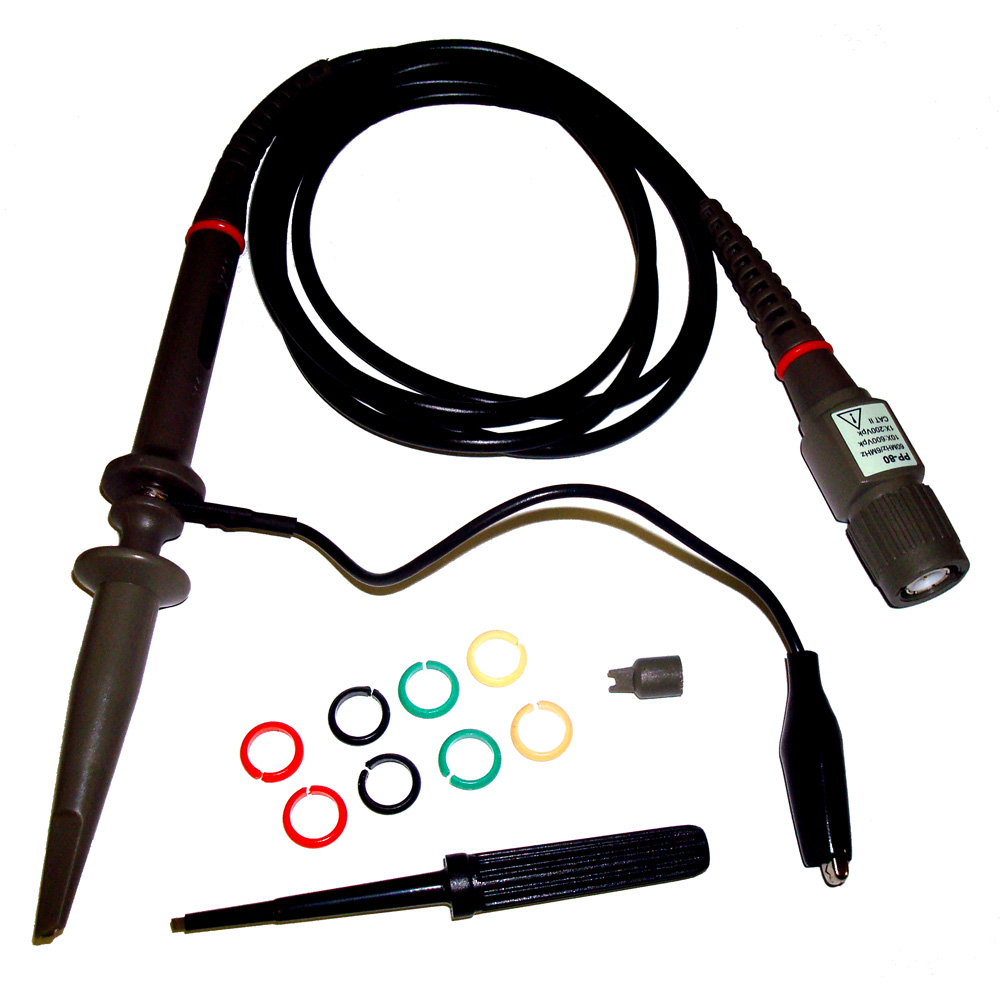
\includegraphics[width=0.45\textwidth]{figs/labs/lissajous/probe.jpg} 
\caption{An example scope probe.}
\label{fig:probe}
\end{center}
\end{figure}

Although we won't be using them in this lab, most sensitive
measurements with an oscilloscope are made using a scope probe, as
shown in Fig.~\ref{fig:probe}.  To protect the circuit being measured
from being affected by the insertion of the probe, there is usually a
large resistance in the probe.  This means that the oscilloscope
itself measures the output of a voltage divider, and the signal is
attenuated, most often by a factor of 10.  The oscilloscope simply
adjusts the voltage scale so that values you read are not attenuated.
To make consistent measurements, you simply have to make sure that the
oscilloscope is configured for the attenuation factor we are using.

In our case, we are connecting coaxial cables directly between the
oscilloscope and the function generator, and so there is no
attenuation.  But the default setup for the scope assumes that you are
using a probe with a $1/10$ attenuation, called a 10X probe.  Look at
the options next to the menu buttons and find the one that says
``Probe 10X Voltage''.  Press this menu button, and then press the
Attenuation button until it reads 1X, appropriate for a coaxial cable
with no attenuation factor.
\begin{figure}[htbp]
\begin{center}
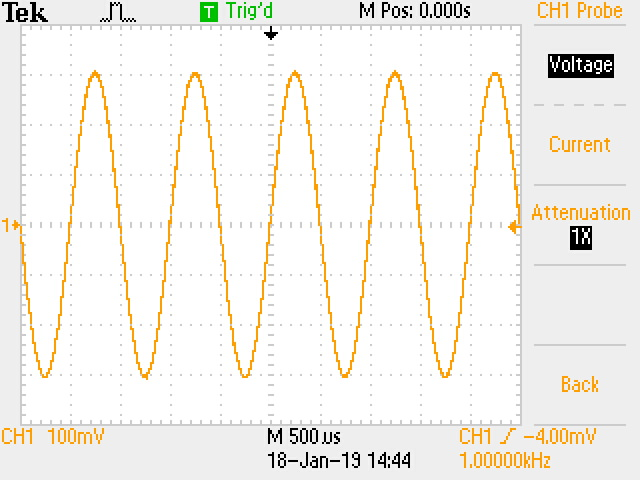
\includegraphics[width=0.45\textwidth]{figs/labs/lissajous/sine.jpg} 
\caption{Correctly scaled scope output.}
\label{fig:scopesine}
\end{center}
\end{figure}
The waveform is unchanged, but now the voltage scale is correctly set
to $100~\rm mV$.  And your signal now appears to be $600~\rm mV$,
consistent with the setting from your function generator, as shown in
Fig.~\ref{fig:scopesine}.  Next turn the knob labeled ``scale'' located
under the yellow channel ``1'' button.  Adjust this knob until the
scale for CH1 is listed as $200~\rm mV$ per division.  The apparent
size of the waveform will be reduced by a factor of two, because each
division is now $200~\rm mV$ and so your $600~\rm mV$ signal appears
three divisions high.

Next note that the function repeats every two divisions.  Since the
time scale is listed as $500~\rm \mu s$, the period is therefore $1~\rm
ms$, corresponding to a frequency of $1~\rm kHz$.  Adjust the time
scale, using the large knob in the Horizontal column, until the time
scale is $100~\rm \mu s$ per division.  This is still a $1~\rm kHz$
signal, but one period now takes up the entire display.

Using the multipurpose knob on your function generator, adjust the
frequency up to $10~\rm kHz$, and observe how the waveform changes.
Then adjust the voltage between about $100~\rm mV$ and $2~\rm V$
peak-to-peak.  When finished, leave the function generator producing a
$5~\rm kHz$ sine wave with $600~\rm mV$ peak-to-peak voltage.  Your
scope should remain at a voltage scale of $200~\rm mV$ and time scale
of $100~\rm \mu s$.  Next, set the DC offset of the signal on the
function generator by pressing:
\begin{displaymath}
{\rm Offset \to 10 \to mV}
\end{displaymath}
Turn the multipurpose knob to adjust the DC offset between $-100~\rm
mV$ and $100~\rm mV$.  Your waveform will rise and fall on your scope
display.  By default, your scope includes the DC offset, but often
this is not what you want.  On your scope, press the button labeled
``Coupling DC'', until the DC becomes AC.  When AC coupled, the DC
component of your waveform is removed.  When AC coupled, observe that
changing the DC offset on the function generator does not change the
position of the waveform.

You can adjust the position of the waveform on your scope display
using the small knobs labeled ``Position'' to adjust the offset in
vertical and horizontal.  Try this out.  To return a waveform to
(0,0), notice that the offset is displayed while you are turning the
knob.

\begin{plot}
Save a scope trace of a sine wave with a non-zero vertical and horizontal
offset. Insert your USB drive into the scope and press the Save button
(it takes few seconds to save).  Whenever you save a scope trace in
this class, make certain that there is a a date printed on the trace.
This ensures that you have your own scope traces, as they can be
confused with those from other sections.
\end{plot}

On your function generator, set the output to a $5~\rm V$ peak-to-peak
sine wave with frequency of $100~\rm kHz$.  Adjust the voltage scale
and time scale until you can clearly see the sine wave.

\section{Lissajous Figures}

\begin{figure}[htbp]
\begin{center}
\begin{tabular}{cc}
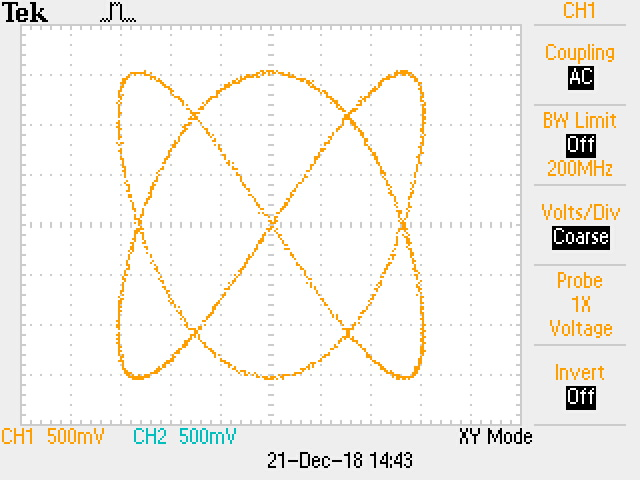
\includegraphics[width=0.45\textwidth]{figs/labs/lissajous/scope_lissajous.jpg} & 
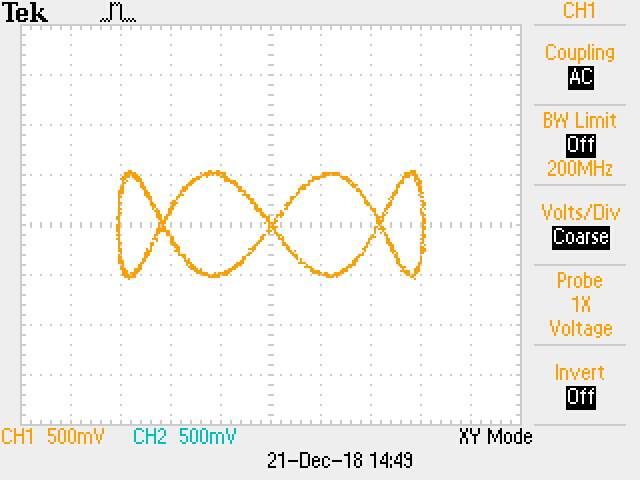
\includegraphics[width=0.45\textwidth]{figs/labs/lissajous/scope_crown.jpg} \\
(a) & (b) \\
\end{tabular}
\caption{Scope traces from Lissajous figures from settings for (a) start, and (b) crown.}
\label{fig:tracelissajous}
\end{center}
\end{figure}
Lissajous figures are the graph of system of two parameterized functions:
\begin{eqnarray*}
x &=& A_1 \sin(2 \pi f_1 t + \delta) \\
y &=& A_2 \sin(2 \pi f_2 t) 
\end{eqnarray*}
which produces a closed loop if the ratio $A_1 / A_2$ is rational.  The appearance of the figure is of a 3 dimensional knot with the viewing angle determined by the parameter $\delta$.  Two examples are shown in Fig.~\ref{fig:tracelissajous}.

To produce these figures on your scope, we'll need to use two
channels.  To begin, enable the output of both Channel 1 and Channel 2
on your function generator, and set them both to produce sine waves
with amplitude $3~\rm V$ peak-to-peak.  Adjust the frequency of
channel 1 to $2~\rm kHz$ and the channel 2 to $3~\rm kHz$.  Note that
you can switch between the Channel 1 and Channel 2 parameter menus on the function generator
with the button labeled ``Ch1/2''.

\begin{figure}[htbp]
\begin{center}
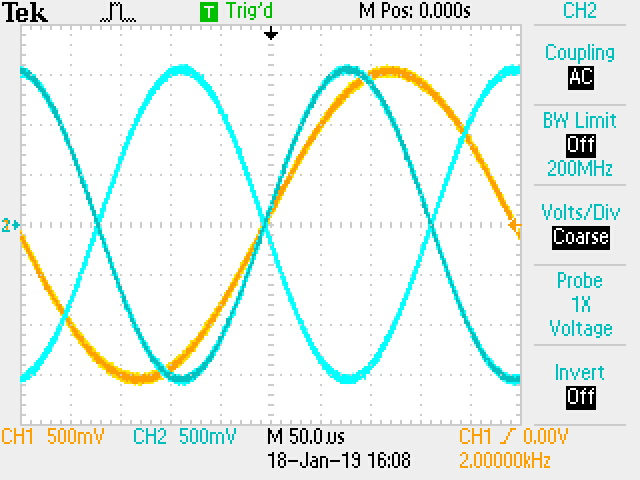
\includegraphics[width=0.45\textwidth]{figs/labs/lissajous/two_sine.jpg} 
\caption{Correctly scaled scope output.}
\label{fig:twosine}
\end{center}
\end{figure}

On your scope, switch to the Channel 2 parameter menu by pressing the
blue button labeled ``2''.  Set the coupling of Channel 2 to AC, and
probe attenuation to 1x, just as you did previously for Channel 1.
Next adjust the voltage scales of each channel to $500~\rm mV$ and set
the common time scale to something appropriate, so that you can view
both Sine waves on the scope display.  As shown in Fig.~\ref{fig:twosine},
you will see two versions of the Channel 2 output, inverted with
respect to each other, because the frequency of Channel 2 is 1.5 times
the frequency of Channel 1. You can check this but changing slightly the frequency of 
Channel 2 but return it to prescribe values to continue with the lab.

The relative phase between the two output channels of your function
generator shifts whenever you adjust the frequency of one of the
signals.  For consistent results with offline plots and the scope
traces shown here, you'll need to align the phase of the two channels
every time you adjust the frequency on the function generator:
\begin{displaymath}
\rm Inter Ch button \to AlignPhase.
\end{displaymath}

Usually, scopes are used to display the inputs as a function of time.
In this case, the voltage level is along the $y$-axis, and time is the
$x$-axis.  This mode is called YT mode.  Occasionally, however, it is
useful to display things in XY mode.  In this mode, the $x$-axis is
used for the voltage of Channel 1 and the $y$-axis is used for the
voltage of Channel 2.  Each point on the curve represents a particular
point in time.  Switch to XY mode by pressing the Display button and
then pressing the button next to the Format menu item until the mode
is XY.  You should reproduce Fig.~\ref{fig:tracelissajous}a
exactly.  If not, check that you have aligned the phase as described
above and that frequencies are set correctly as in Table.

\begin{table}
\begin{center}
\caption{Settings for various Lissajous figures.}
\label{tbl:lissajous}
\begin{tabular}{llll}
pattern & $f_1~\rm(kHz)$ & $f_2~\rm(kHz)$ & $\delta_1$ \\
start & 2 & 3 & 0 \\
fish & 2 & 3 & $135^\circ$ \\
parabola & 1 & 2 & $45^\circ$ \\
lace & 13 & 12 & 0 \\
crown & $1~\rm kHz$ & $4~\rm kHz$ & 0 \\
\end{tabular}
\end{center}
\end{table}

\begin{plot}
Adjust the phase of Channel 2, under menu item StartPhase, until the
pattern collapses into a Fish pattern (or greek letter $\alpha$) at
135 degrees.  Save a scope trace.
\end{plot}

\begin{plot}
Produce the parabola pattern according to the settings in
Table~\ref{tbl:lissajous}, saving a scope trace.  Remember to align
the phase each time you change the frequency.
\end{plot}

\begin{plot}
Produce lace pattern and save a scope trace.
\end{plot}

\begin{plot}
Produce the crown pattern, shown in Fig.~\ref{fig:tracelissajous}b.
For the right proportions, adjust the amplitude of Channel 2 to $1~\rm
V$ peak-to-peak, leaving Channel 1 at $3~\rm V$ peak-to-peak.  Notice
that as you adjust the phase of Channel 1, the crown appears to
rotate.  Adjust the frequency of Channel 2 to $4.0002~\rm kHz$.  The
crown should now appear to rotate constantly at low speed.
\end{plot}

This is a \textbf{sign-off point} for this lab. 

Please return all the components you took and cables to their
place. Leave you workstation clean.

\section{Lissajous Figures Analysis}

If you run out of time, you can finish the remaining portion of this
lab, which is exclusively done in Jupyter notebook, at another time,
such as during the Friday open lab period.  Just make sure you have
saved all of your oscilloscope traces.

Include your two scope traces in the python notebook. Make sure the
date is clearly visible on each plot. Provide a full label for each
plot which describes all the relevant information.  You can display
your scope traces in python using the Image library like this:

\begin{verbatim}
      from IPython.display import Image

       image = Image(filename='myscope.jpg') 
       display(image)
\end{verbatim}
This assumes that you copied your scope traces inside the jupyter notebook directory. 

\begin{plot} Reproduce fish pattern using scientific
python to draw the parameterized shape.  For
example, see Fig.~\ref{fig:pythonlissajous}. \end{plot}
\begin{plot} Reproduce  parabola pattern. \end{plot} 
\begin{plot} Reproduce crown pattern. \end{plot}

One way to approach this problem is to set the period to $1~\mu s$.
The functions should be evaluated at 1000 discrete times within the
interval from 0 to $1~\mu s$.
\begin{verbatim}
     t = np.linspace(0,1,num=1000)
\end{verbatim}
Define a fundamental angular frequency $\omega_0 = 2 \pi~\rm kHz$:
\begin{verbatim}
     w = 2*np.pi
\end{verbatim}
With these definitions, we would define:
\begin{verbatim}
     x = np.sin(4*w*t)
\end{verbatim}
to obtain $x$ points corresponding to $f=4~\rm kHz$ sine function.

When plotting your curves, use:
\begin{verbatim}
       plt.axis('equal')
\end{verbatim}
to keep the unit aspect ratio used by your scope.

\begin{figure}[htbp]
\begin{center}
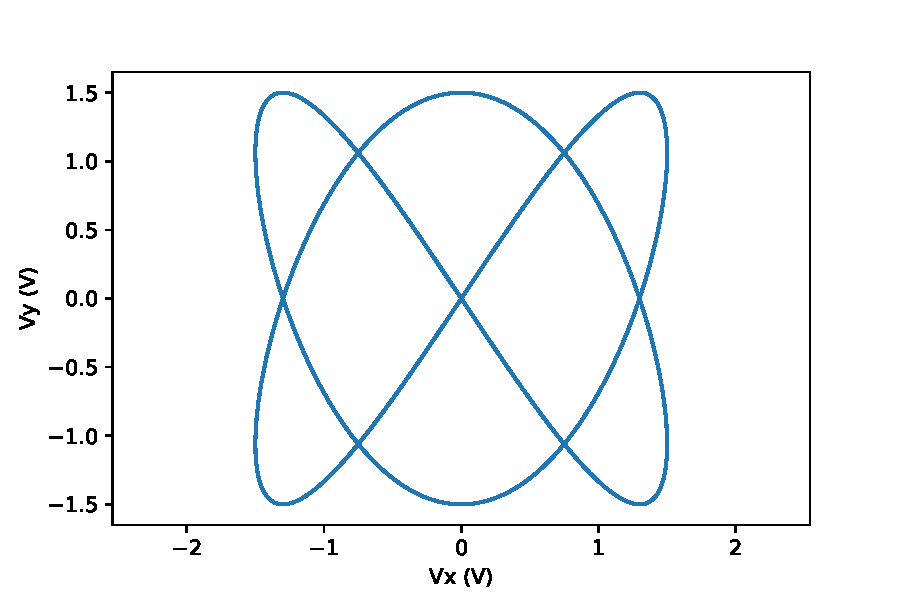
\includegraphics[width=0.45\textwidth]{figs/labs/lissajous/pythonlissajous.pdf} 
\caption{Lissajous curve constructed using Scientific Python corresponding to the scope trace in Fig.~\ref{fig:tracelissajous}a.}
\label{fig:pythonlissajous}
\end{center}
\end{figure}

\chapter{RC and RL Transient Signals}


\section{Introduction}

In this lab you will use explore transient behavior of$RC$ and $RL$ circuits.  You will learn
how to use scope probes and measure properties of waveforms on your digital oscilloscope using cursors.  For this lab there are both logbook and jupyter notebook entries.


%\section{Pre-lab Calculation}
%
%\noindent
%1) Show that for an exponential decay with time constant $\tau$, the rise-time, when defined as the time interval between $10\%$ and $90\%$ values, is given by:
%\begin{displaymath}
%t_{90} = {\rm ln}(9) \; \tau \sim 2.2 \; \tau
%\end{displaymath}
%
%\noindent
%2) Calculate the inductance of a solenoid with N=20 turns, length $\ell=4~\rm cm$, a radius of $1~\rm cm^2$ using the formula:
%\begin{displaymath}
%L = \frac{\mu_0 N^2 A}{\ell}
%\end{displaymath}
%where $A$ is the cross-sectional area and $\mu_0 = 1.257 \times 10^{-6}~\rm H/m$.


\section{Transient Response of an $RC$ Circuit}

\begin{figure}[htbp]
\begin{center}
\begin{tikzpicture}
    \node[anchor=south west,inner sep=0] (image) at (0,0,0)
         {\includegraphics[height=0.30\textheight]{figs/labs/transients/probe_setup.jpg}};
         \node[left](X) at (-1.0,4.0) {Probe Tip}; \draw (X.east) --
         (5.0,2.4); \node[left](X) at (-1.0,3.0) {Ground Clip}; \draw
         (X.east) -- (5.4,2.2); \node[right](X) at (10.0,5.0) {BNC
           Tee}; \draw (X.west) -- (8.0,5.2); \node[right](X) at
         (10.0,4.0) {Alligator pair}; \draw (X.west) -- (6.5,2.8);
\end{tikzpicture}
\caption{A setup for connecting the scope probe directly to the output of the function generator.}
\label{fig:probe_setup}
\end{center}
\end{figure}

Set your Channel 1 of your function generator to produce Square wave
output with a peak-to-peak voltage of $6~\rm V$ and a frequency of
$1~\rm kHz$.  As shown in Fig.~\ref{fig:probe_setup}, use a BNC Tee adapter
to split the output into two copies.  Send one copy directly to the
Channel 1 input of your scope.  Send the other copy to a
BNC-alligator-pair cable.  

Install an oscilloscope probe at Channel 2 of your scope (see Fig~\ref{fig:probe}).  Some probes
in the lab have the ability to switch between attenuation factors near
the probe tip.  If you have such a probe, select the 10X setting.  The
remaining probes have a fixed attenuation of 10X.

So far, we haven't had to worry about proper grounding procedure,
because this is automatically handled by the BNC cable.  Your scope
probe has two main parts, the larger probe tip, which slides to reveal
a hook which can be attached to wires and components in your circuit,
and a short lead ending with a black alligator clip called the
``Grounding clip''.  Handheld devices like your DMM have no connection
to earth ground.  The voltage reference point at the Common terminal
can be connected anywhere you would like in a circuit.  Your scope is
quite different!  It plugs into a wall outlet for power and is
referenced to earth ground.  To provide a scope which is both safe and
cost effective, most scopes are limited to making measurements which
are referenced to ground when using ordinary probes.  The ground clip
of your scope can only be connected to earth ground.  If you connect
it anywhere else in your circuit, that part of your circuit will be
short-circuited to ground.

For now, connect the probe directly to the output of the
function generator.  Your function generator is also referenced to
earth ground.  In particular for this setup, the black alligator clip
is earth ground.  Connect the black clip from the function generator
to the grounding clip for the scope probe.  Next connect the scope
probe to the red alligator clip from the function generator.  You now
have two copies of the function generator output being sent to the
scope.  One directly through the BNC cable, and one through a 10X
attenuation scope probe.

Adjust your scope to view the function generator output as measured by
Trigger 1.  Set the voltage scale as large as possible while observing
the entire wave form.  Leave the timescale at the default setting of
$500~\mu s$ for now.  Check that trigger is on the Falling edge, as set
in the last section.  Set the trigger near threshold near 0 volts.
You should observe that the position of the waveform does not vary
much with trigger threshold: the steep falling edge of the square wave
function gives us a solid reference point for defining $t=0$ in the
measurements that follow.

Now enable Channel 2 on your scope. Adjust all the necessary setting for Channel 2. It should be an identical copy of
Channel 1.  Too see both channels at the same time, you'll have to
move the vertical position of Channel 1 slightly. Closed loop tests
like this are the way experienced scientists and engineers always
start.  It allows you to setup your signal generator and scope
properly, without adding the complexity of the circuit you are working
on.  In general, avoiding confusion by taking small incremental steps
is the fastest, most reliable way to proceed in lab.  

\begin{figure}[htbp]
\begin{center}
\begin{tabular}{cc}
\begin{circuitikz}[line width=1pt]
\draw (0,0) to[square voltage source,bipoles/length=1.5cm] ++(0,4.0) to[short] ++(2.0,0)
to[R,-*] ++(0,-2.0) coordinate(X) to[short,*-o] ++(1.0,0) node[right]{A};
\draw (X) to[C,-*] ++(0,-2.0) coordinate(X) to[short,-o] ++(1.0,0) node[right]{B};
\draw (X) to[short,-*] ++(-2.0,0) node[ground,yscale=2.0]{};
\end{circuitikz}  &
\begin{circuitikz}[line width=1pt]
\draw (0,0) to[square voltage source,bipoles/length=1.5cm] ++(0,4.0) to[short] ++(2.0,0)
to[R,-*] ++(0,-2.0) coordinate(X) to[short,*-o] ++(1.0,0) node[right]{A};
\draw (X) to[L,-*] ++(0,-2.0) coordinate(X) to[short,-o] ++(1.0,0) node[right]{B};
\draw (X) to[short,-*] ++(-2.0,0) node[ground,yscale=2.0]{};
\end{circuitikz}  \\
(a) & (b) \\
\end{tabular}
\caption{A function generator driving an (a) RC circuit, and (b) RL circuit.}
\label{fig:rlc-circuits}
\end{center}
\end{figure}


Construct the circuit in Fig.~\ref{fig:rlc-circuits}a on your
breadboard, as shown in Fig.~\ref{fig:rc_setup}a.  Use $C=10~\rm nF$
capacitor and $R=10~\rm k\Omega$.  
\begin{measurement} Using the given values of resistor and capacitor, calculate and record in your logbook the time constant of the RC circuit  together with its minimum and maximum value assuming 5\% tolerance. Take care to include proper units. Using your DMM, measure and record
the actual resistance and capacitance of your components before
installing them. Record each value together with accuracy of your DMM for that specific measurement (see table~\ref{tbl:accuracy}). Then calculate the time constant of the RC circuit using the measured values. We still did not learn how to propagate uncertainties. Estimate which fractional uncertainty ($\mbox{accuracy of a value}/\mbox{measured value}$) is larger and apply this fractional uncertainty to your calculated time constant. Do the ranges for the estimates of time constant overlap? Add a comment in your logbook. \end{measurement}

 Use your function generator as the square wave
voltage source.  Recall that the black alligator clip is earth ground.
The red alligator clip is the square wave output relative to earth
ground, and corresponds to the upper terminal of the voltage source in
the diagram.  The only valid place to connect the grounding clip of
your scope probe is to earth ground, so connect that to point B in
your circuit.  Connect the scope probe tip to point A.  As shown in
the Fig.~\ref{fig:rc_setup}b, each time the square wave changes
polarity, the capacitor beings charging or discharging until it
reaches equilibrium with the new voltage, revealing the characteristic
exponential transient response.

\begin{figure}[htbp]
\begin{center}
\begin{tabular}{cc}
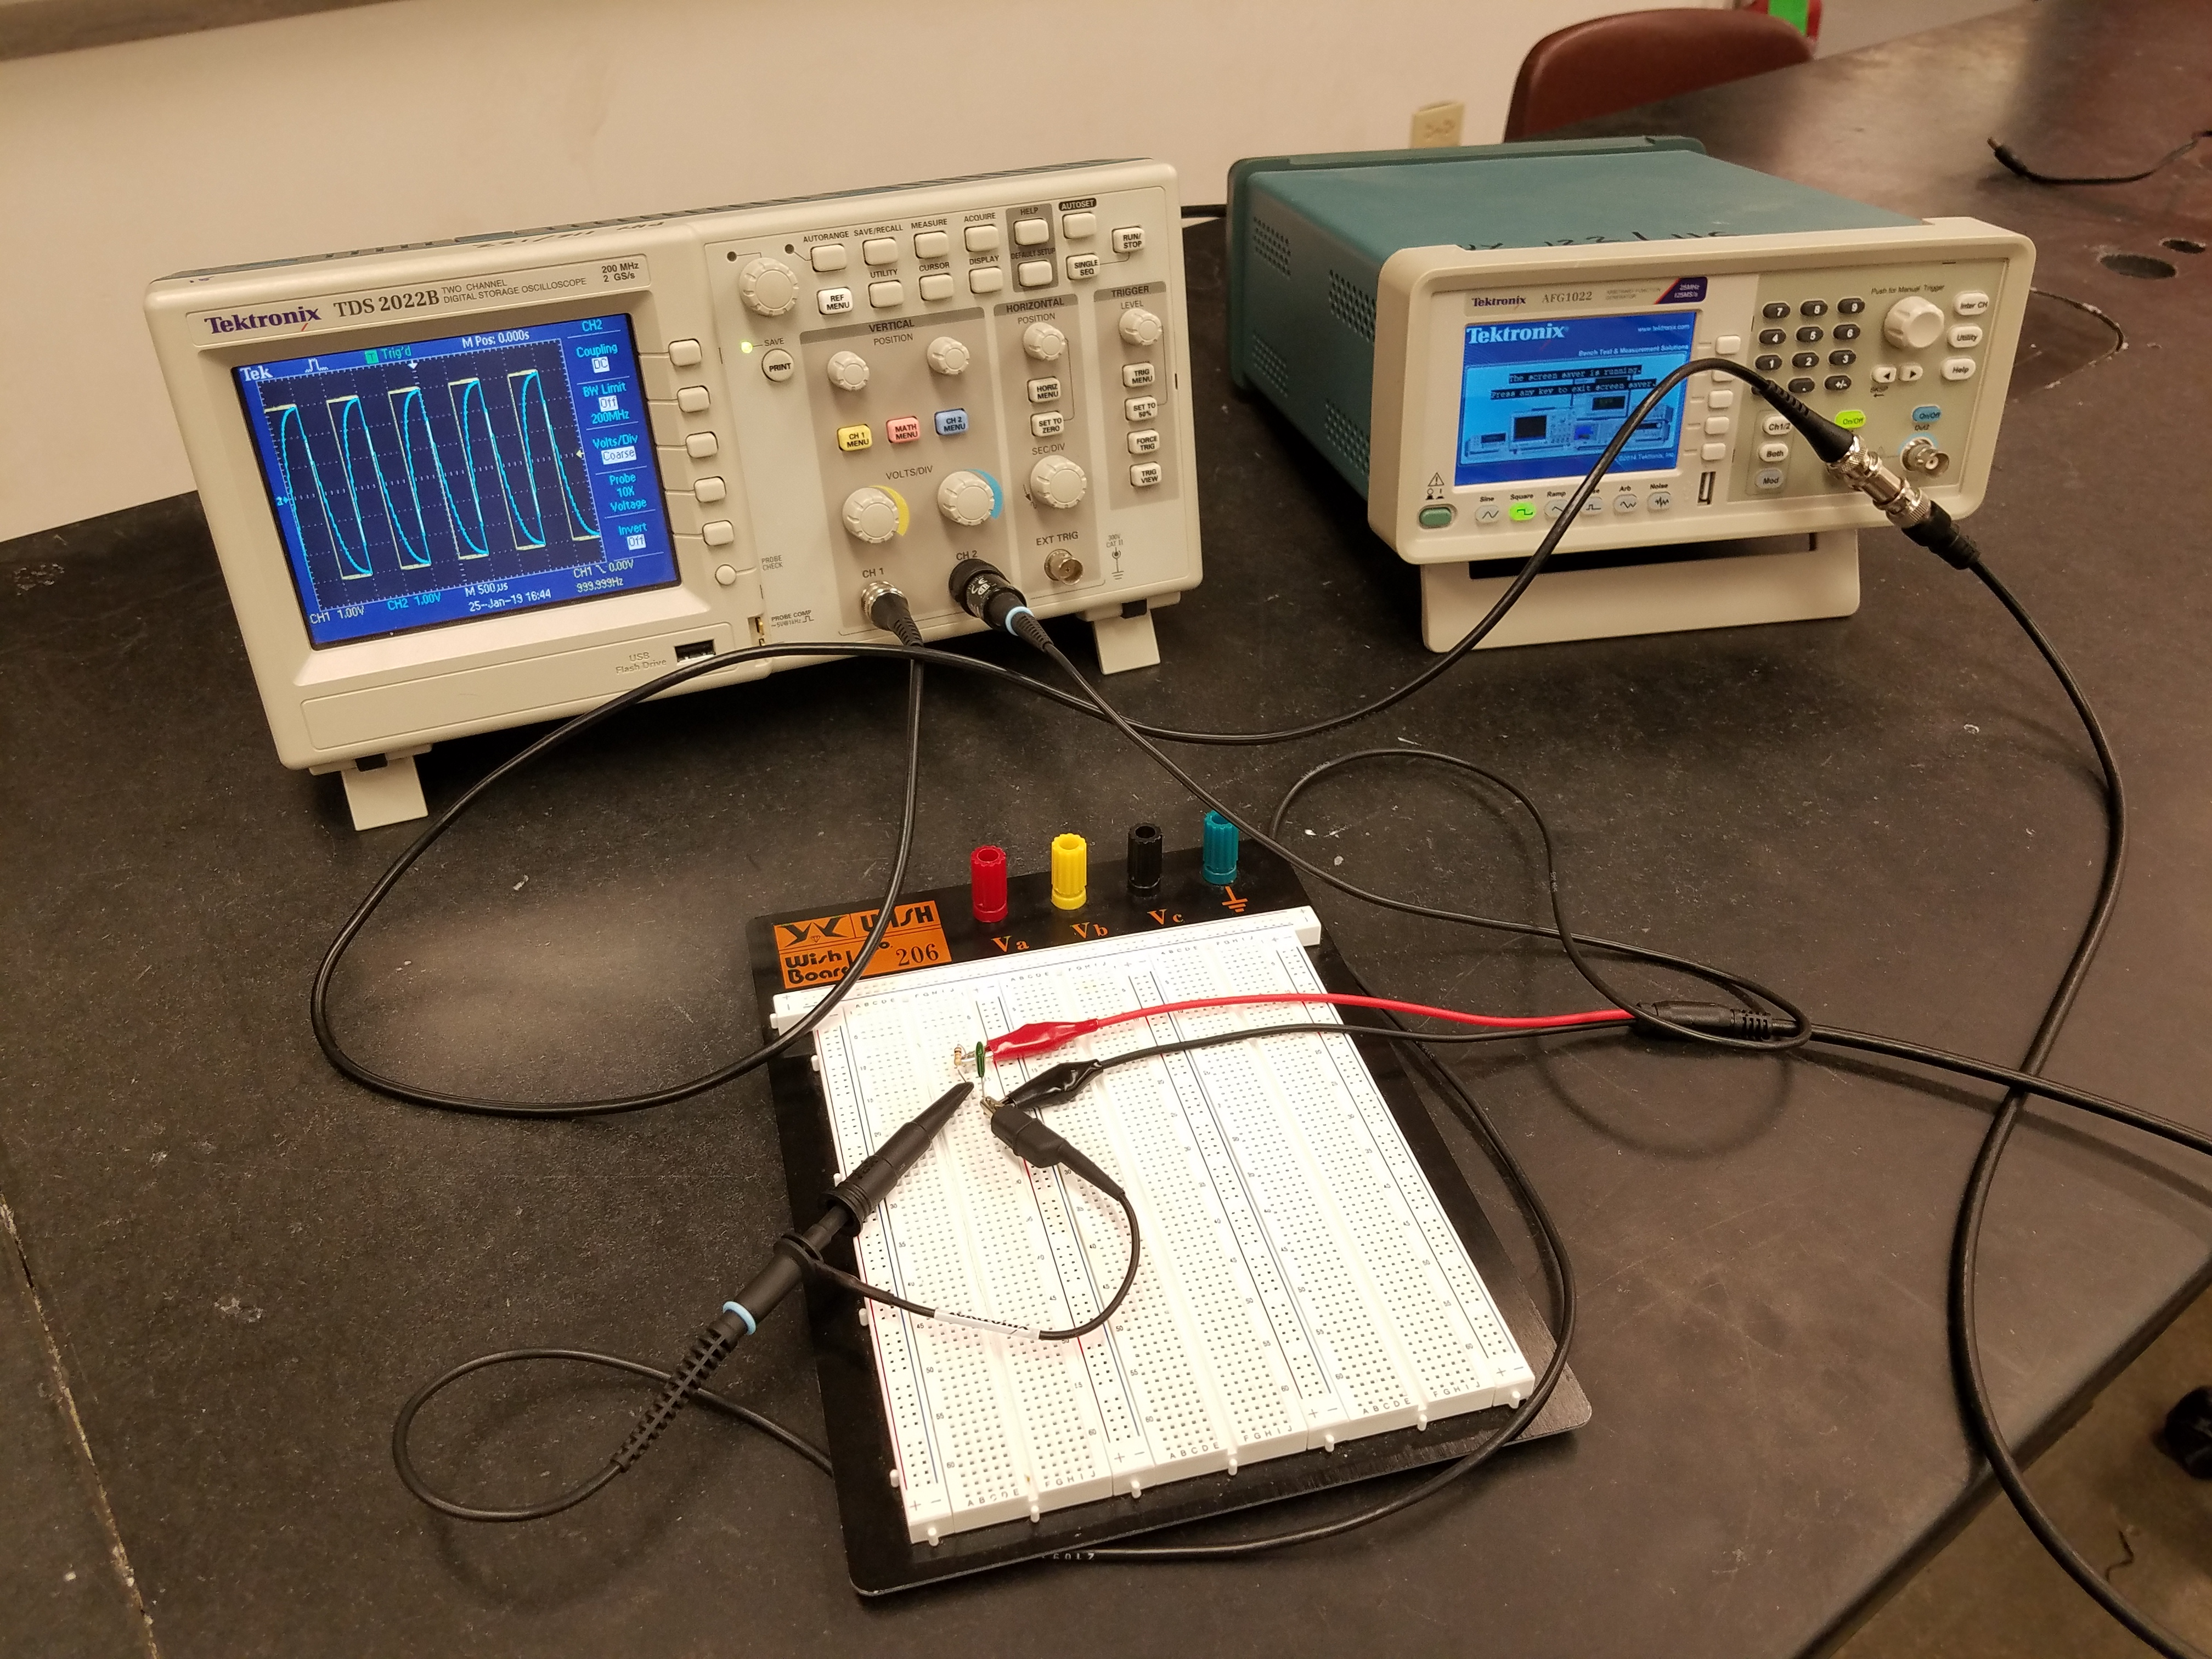
\includegraphics[width=0.45\textwidth]{figs/labs/transients/rc_setup.jpg} &
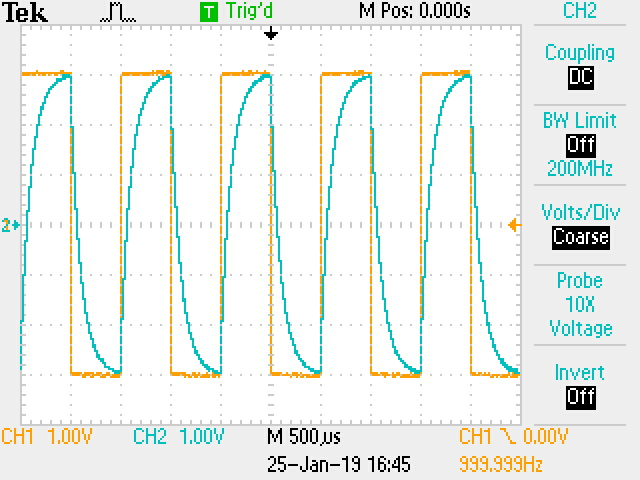
\includegraphics[width=0.45\textwidth]{figs/labs/transients/rc_trace.jpg} \\
(a) & (b) \\
\end{tabular}
\caption{Setup for the (a) RC circuit measurement, and (b) example scope trace showing exponential curve.}
\label{fig:rc_setup}
\end{center}
\end{figure}

\begin{figure}[htbp]
\begin{center}
\begin{tabular}{cc}
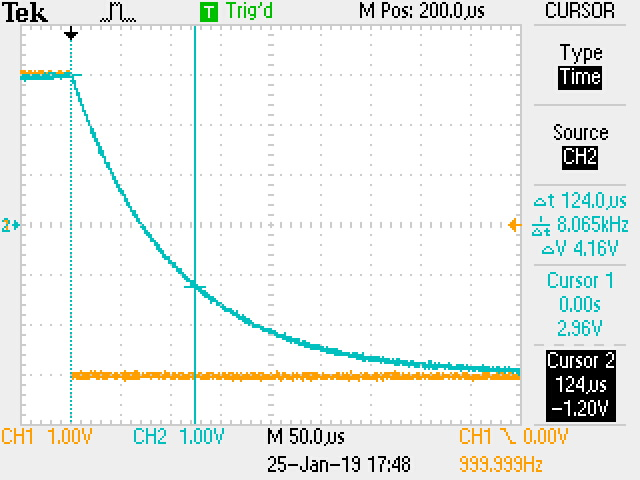
\includegraphics[width=0.45\textwidth]{figs/labs/transients/rc_cursor.jpg} &
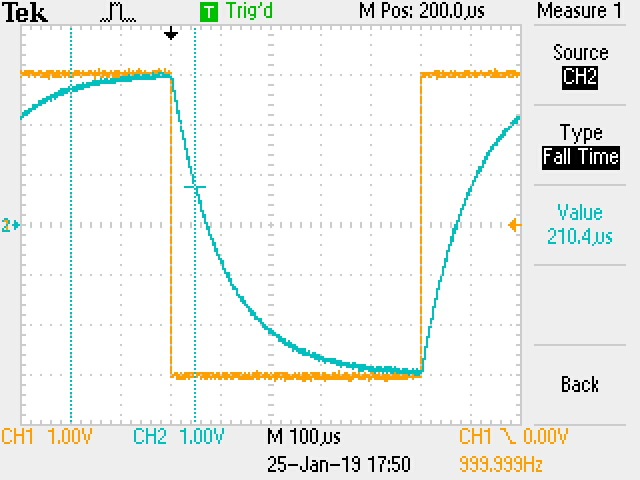
\includegraphics[width=0.45\textwidth]{figs/labs/transients/rc_falltime.jpg} \\
(a) & (b) \\
\end{tabular}
\caption{Scope traces showing (a) use of cursor to measure the waveform at $t=124~\rm \mu s$ and $V=-1.20~\rm V$, (b) use of the built in fall time measurement.}
\label{fig:cursor_falltime}
\end{center}
\end{figure}

Now adjust the timescale to zoom in on the exponential decay portion
of the curve, making sure to keep the trigger position at the left
side of the display, as shown in Fig.~\ref{fig:cursor_falltime}a.
Press the Cursor button, then set Type to Time, and Source to CH2.
This feature allows you to make measurements of different points along
the curve.  Leave Cursor 1 located at $t=0$.  Highlight Cursor 2, by
pressing the corresponding menu button, and adjust it's position using
the multipurpose knob.  Now you can make accurate measurements of the
waveform by reading off the voltage and time at anywhere that you
place the cursor.  
\begin{measurement} Record one measurement every $\sim 25~\rm \mu s$
starting from $t=0~\mu s$ to $400~\rm \mu s$.  (Recall that when
making measurements at target values, you need not hit the target
value exactly, simply record the actual position at which you made
your measurement.) Record also the sketch of your setup and the rough sketch of your waveform.\end{measurement}

\begin{measurement} Your scope can also directly measure the fall time of a waveform.
Setup the function so that one complete falling edge is on screen, as
shown in Fig.~\ref{fig:cursor_falltime}b.  Press Measure and then set
source to CH2 and Type to ``Fall Time''. You might see this value fluctuating. Record five measurements of this value in your logbook.\end{measurement}


\begin{measurement}
Show in your logbook that for an exponential decay with time constant $\tau$, the rise-time, when defined as the time interval between $10\%$ and $90\%$ values, is given by:
\begin{displaymath}
t_{90} = {\rm ln}(9) \; \tau \sim 2.2 \; \tau
\end{displaymath}
\end{measurement}

\begin{plot} Using the above relation and five measurements of fall time calculate the mean value of the time constant of the RC circuit. Recall you can use numpy functions. Calculate also the standard error of the mean value as following: $\sigma_{mean}= \mbox{standard deviation}/\sqrt{\mbox{number of measurements}}$.
\end{plot} 

\begin{measurement} Record the third estimate for the time constant of the RC circuit together with uncertainty in your logbook. Examine now all three different estimates. Are they consistent? Do the ranges for the three estimates of the time constant overlap? Add comment in your logbook about how those estimates compare to each other. Also record your qualitative understanding of this comparison. 
\end{measurement}


% Check that the measured fall time is consistent with your measured values of $R$ and $C$, using the formula from prelab. 


\section{Analysis}

\begin{plot} Plot your collected $RC$ circuit exponential decay data as discrete
data points and compare with the expected exponential decay function
as a continuous curve using the expected $RC$ time constant calculated
from: 1) given value of $R$ and $L$ (Prediction 1), 2) your measured value of $R$ and $L$ (Prediction 2) and 3) your measured value of the fall time via scope (Prediction 3).  Make sure to have
appropriate axis labels and a legend indicating ``Data'',``Prediction 1'', "Prediction 2" and "Prediction 3". 
Describe (in your jupyter notebook) how those predictions are matching your measured data? Could you tell which prediction describes your data best?
\end{plot}

\begin{plot} Redo the plot (in a new inline plot) using a log scale with base of 10 in y axis. To apply logarithmic scale explore the options for plotting in python. A logarithmic scale is a nonlinear scale often used to represent a large range of positive values. You will have to make your voltage measurements larger than zero and you can do this by shifting the measured values by a constant factor. On a logarithmic scale each increment on the axis increases by a factor of 10. On a linear scale each increment on the axis increases by equal fixed increment.  
On a linear scale, a change between two values is perceived as the difference between the values. For example, a change from 1 to 2 is the same amount of increase as from 99 to 100. On a logarithmic scale, a change between two values is perceived as the ratio of the two values. For example, a change from 1 to 2 (ratio of 1:2) is the same amount of increase as a change from 50 to 100 (also a ratio of 1:2). Describe (in your jupyter notebook) how those predictions are matching your measured data? Could you tell which prediction describes your data best? Is this plot more informative? Add these comments to your jupyter notebook. 
\end{plot}

\begin{plot} Plot a difference between data and different prediction as data points in a separate plot. This is so called residual plot. Make sure to have appropriate axis labels and a legend indicating ``Data - Prediction 1'',``Data - Prediction 2'', "Data - Prediction 3".  Recall that you will have to cast your predictions in arrays. Describe (in your jupyter notebook)  how those predictions are matching your measured data? Could you tell which prediction describes your data best? Is this plot more informative? Add these comments to your jupyter notebook. 
\end{plot}



\noindent
This is a \textbf{sign-off point} for this lab. 

\section{Transient response of an RL circuit}


\begin{measurement}
Calculate the inductance of a solenoid with N=20 turns, length $\ell=4~\rm cm$, a radius of $1~\rm cm^2$ using the formula:
\begin{displaymath}
L = \frac{\mu_0 N^2 A}{\ell}
\end{displaymath}
where $A$ is the cross-sectional area and $\mu_0 = 1.257 \times 10^{-6}~\rm H/m$.
\end{measurement}

\begin{measurement}
Wrap an inductor around the provided wooden dowel. Estimate it's
inductance by modifying your calculation above accordingly and record the value in your logbook.  Using your DMM, measure and record the actual resistance. You can skip to estimate accuracy for this measurement.
\end{measurement}


\noindent Turn down the supply to $2.5~\rm V$ peak-to-peak.  Build the circuit in
Fig.~\ref{fig:rlc-circuits}b using your homemade inductor and a
resistor of $R=47~\rm Ohms.$ 
\begin{measurement}
Measure the fall-time of your R-L circuit
and use it to determine a measured value for the inductance.
Determine and record the inductance of your coil and compare to your theoretical
estimate. Add a comment in your logbook. 
\end{measurement}

\chapter{Passive Filters}

\section{Introduction}

In this lab, you will build and measure the performance of a low-pass
and a high-pass $RC$ filter, and produce Bode plots to compare your
circuit with the impedance model derived in class and shown in
Fig.~\ref{fig:bode}.  For this lab there are both logbook and jupyter notebook entries.


\begin{figure}[htbp]
\begin{center}
%\begin{tabular}{c@{\hskip 0.25in}c}
\begin{tabular}{cc}
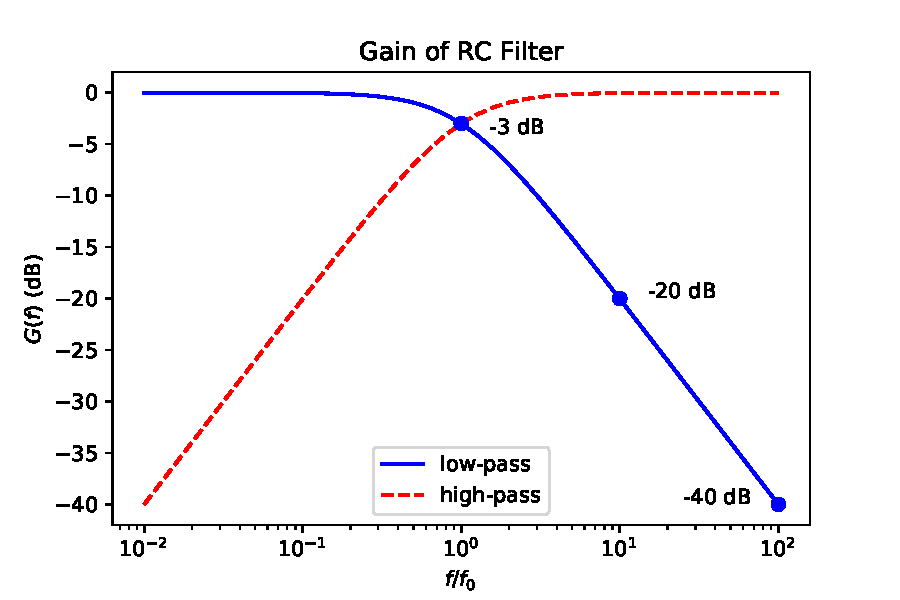
\includegraphics[height=0.22\textheight]{figs/labs/filters/rcgaindb.pdf}
&
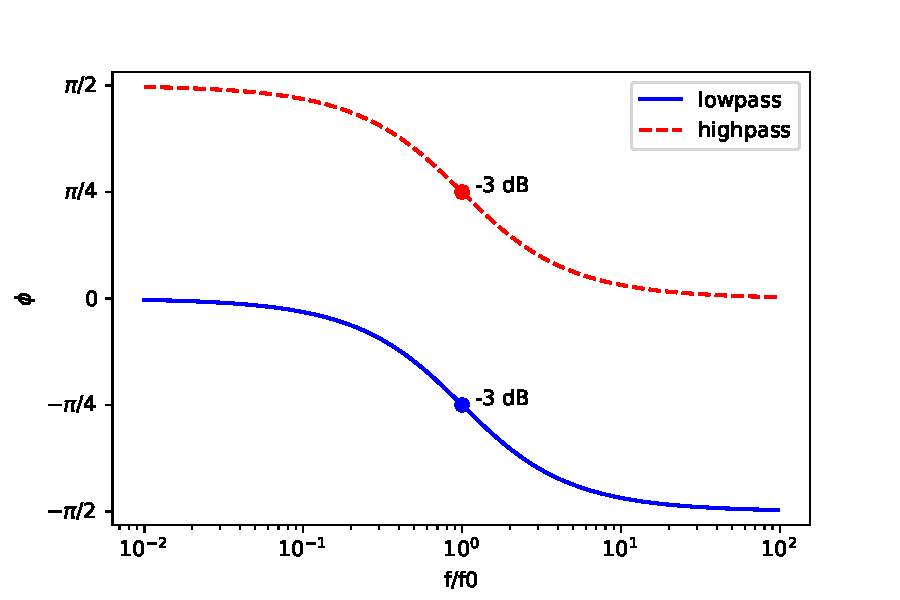
\includegraphics[height=0.22\textheight]{figs/labs/filters/rcphase.pdf} \\
(a) & (b) \\
\end{tabular}
\end{center}
\caption{\label{fig:bode} Bode plots for high-pass and low-pass filters showing the (a) gain on a dB scale, and (b) phase, both as a function of the ratio of frequency $f$ to the crossover frequency $f_0$ on a log scale.}
\end{figure}


\begin{figure}[htbp]
\begin{center}
\begin{tabular}{c@{\hskip 2cm}c}
\begin{circuitikz}[line width=1pt]
\draw (0,0) to[sinusoidal voltage source,bipoles/length=1.5cm] ++(0,4.0) to[short] ++(2.0,0) coordinate(X) to[short,*-o] ++(1.0,0) node[right]{C};
\draw (X) to[R,-*,l=$R_1$] ++(0,-2.0) coordinate(X) to[short,*-o] ++(1.0,0) node[right]{B};
\draw (X) to[C,-*,l=$C_1$] ++(0,-2.0) coordinate(X) to[short,-o] ++(1.0,0) node[right]{A};
\draw (X) to[short,-*] ++(-2.0,0) node[ground,yscale=2.0]{};
\end{circuitikz}  &
\begin{circuitikz}[line width=1pt]
\draw (0,0) to[sinusoidal voltage source,bipoles/length=1.5cm] ++(0,4.0) to[short] ++(2.0,0)coordinate(X) to[short,*-o] ++(1.0,0) node[right]{C};
\draw (X) to[C,-*,l=$C_1$] ++(0,-2.0) coordinate(X) to[short,*-o] ++(1.0,0) node[right]{B};
\draw (X) to[R,-*,l=$R_1$] ++(0,-2.0) coordinate(X) to[short,-o] ++(1.0,0) node[right]{A};
\draw (X) to[short,-*] ++(-2.0,0) node[ground,yscale=2.0]{};
\end{circuitikz}  \\
(a) & (b) \\
\end{tabular}
\caption{\label{fig:rc_circuits}
Circuit diagrams for $RC$ (a) low-pass filter and (b) high-pass filter.
The input voltage is $V_{\rm in} = V_{\rm AC}$ while the output voltage is $V_{\rm out} = V_{\rm AB}$.}
\end{center}
\end{figure}


\section{Low-pass Filters}

\begin{figure}[htbp]
\begin{center}
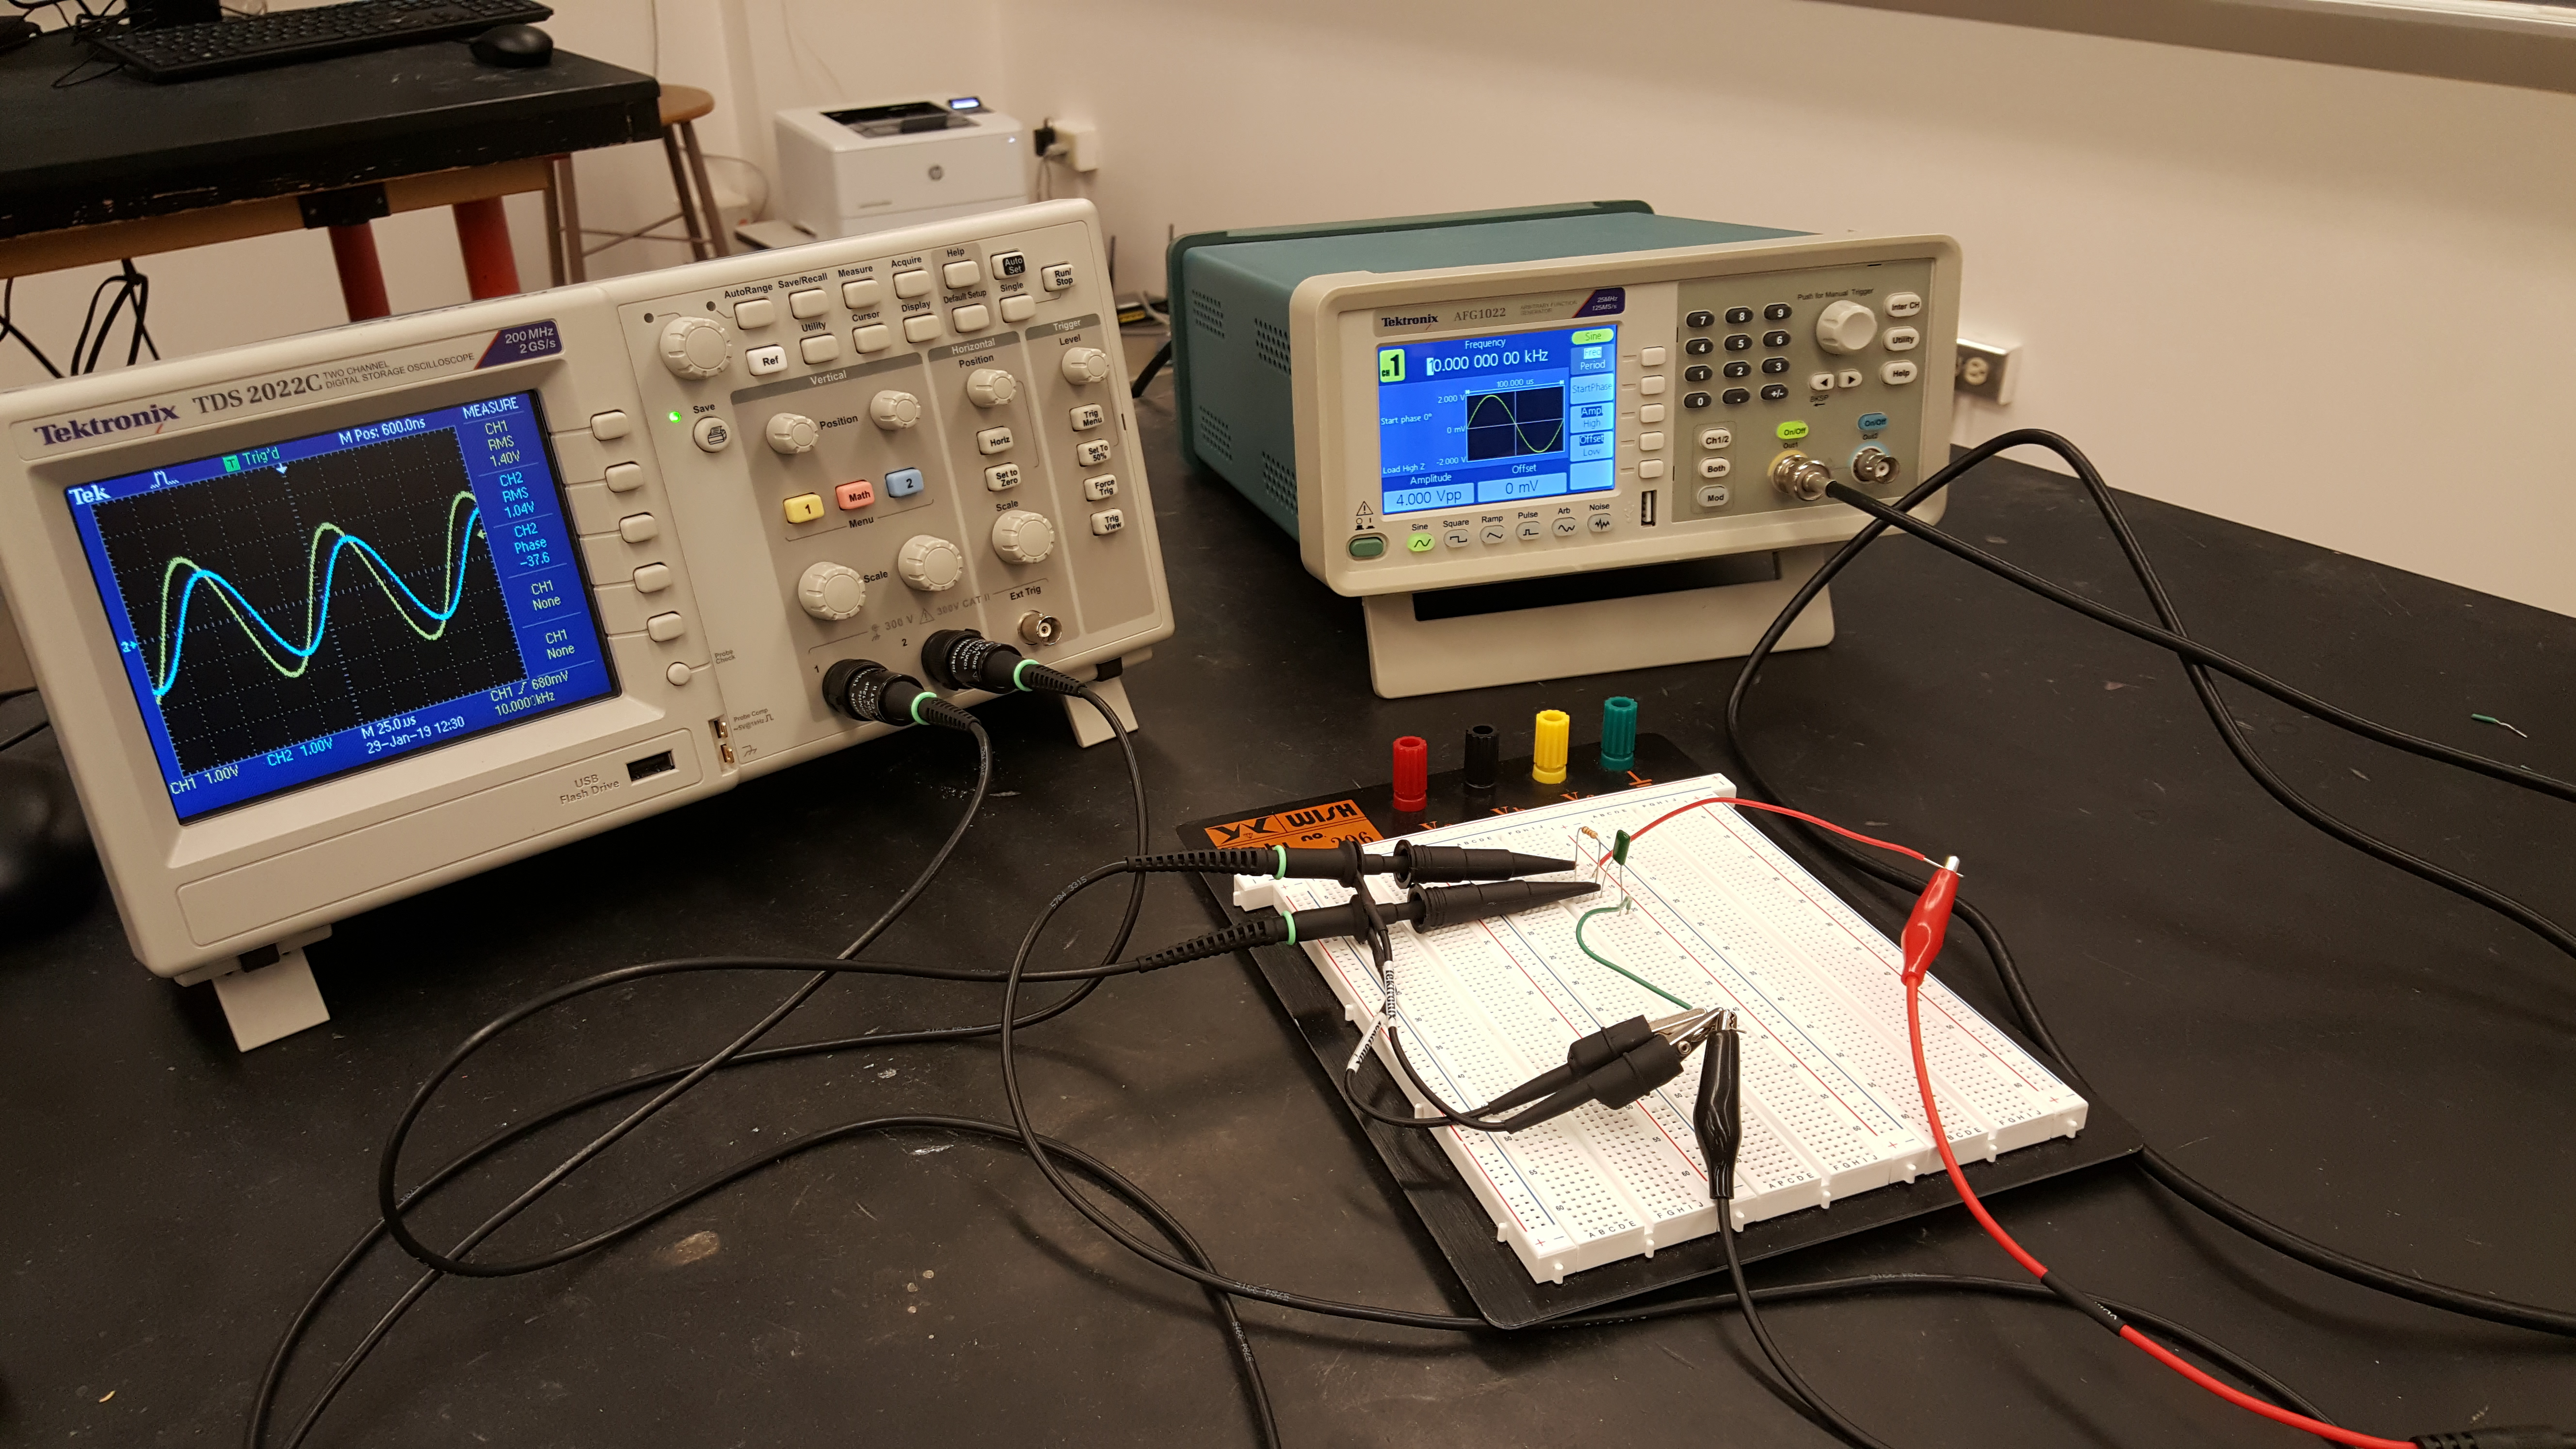
\includegraphics[height=0.22\textheight]{figs/labs/filters/filter_setup.jpg}
\end{center}
\caption{\label{fig:filter_setup} Setup for RC low-pass filter.}
\end{figure}


\begin{measurement} Calculate the corner frequency $f_0$ (aka the frequency of
$-3~\rm dB$ point) for the RC filters shown in
Fig.~\ref{fig:rc_circuits} for $R_1=1.5~\rm k\Omega$ and $C_1=10~\rm nF$.\\
\end{measurement}
\noindent Set your function generator to produce a sine function with a
peak-to-peak voltage of $4~\rm V$ and set the frequency to the calculated value of the corner frequency. %$10~\rmkHz$.  
Build the circuit shown in Fig.~\ref{fig:rc_circuits}a using
$R=1.5~\rm k \Omega$ and $C= 10~\rm nF$.  
\begin{measurement} Measure and record the
actual resistance and capacitance of the components before installing
them in your circuit. 
\end{measurement}
Use a BNC-alligator-pair cable to connect the
function generator output to your breadboard, to provide the AC
voltage source.  Keep in mind that the black alligator clip from your
function generator is earth ground, while the red alligator clip is the
function generator output referenced to ground, i.e. the top of the AC
source as drawn in the circuit diagram.

You will be using two scope probes in this lab, and as always some
care must be taken with respect to grounding when using your scope.
Your function generator has already set the earth ground point in your
circuit at the black alligator clip, which is point A in the circuit
diagram.  The scope grounding clips should both be connected to point
A.  To measure $V_{\rm in}$ on your scope Channel 1, connect the scope
probe tip of Channel 1 to point C in your circuit.  To measure $V_{\rm
  out}$ on your scope Channel 2, connect the scope probe tip of
Channel 2 to point B in your circuit.

The setup, including the scope, is illustrated in
Fig.~\ref{fig:filter_setup}.  Note in particular that the two scope
grounding clips and function generator ground are all connected to a
single (green) wire, which is used to set the ground point in the
circuit.

Set your Scope to the default setup, then adjust the timescale
appropriately and enable the output of channel 2.  
\begin{measurement} Calculate at $1\%$
precision the corner frequency $f_0$ from the measured values of your
resistor and capacitor, and set the frequency of your function
generator to that value. 
\end{measurement}

\noindent To produce the Bode plots for your filter,
we will be measuring the voltage gain $G = V_{\rm out} / V_{\rm in}$
and the phase shift $\phi$ of $V_{\rm out}(t)$ relative to $V_{\rm
  in}(t)$.

\begin{figure}[htbp]
\begin{center}
\begin{tabular}{cc}
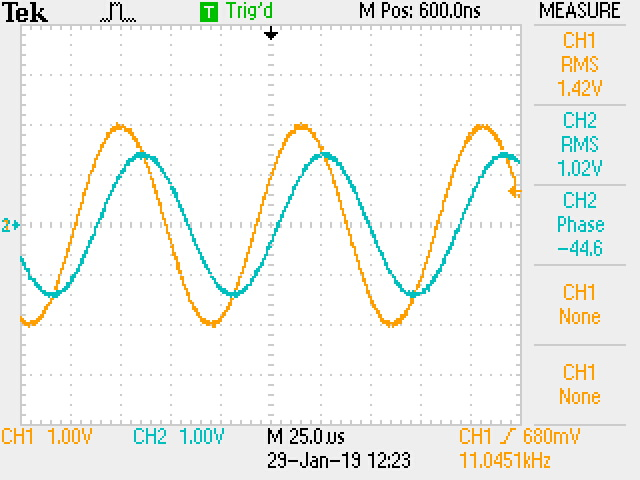
\includegraphics[width=0.4\textwidth]{figs/labs/filters/phase_measure.jpg} &
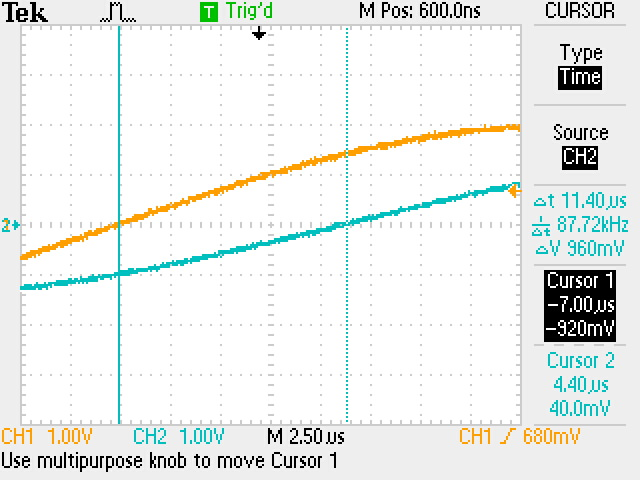
\includegraphics[width=0.4\textwidth]{figs/labs/filters/phase_cursor.jpg} \\
(a) & (b) \\
\end{tabular}
\end{center}
\caption{\label{fig:scopegain} Measuring the gain and phase with your scope.}
\end{figure}

The gain is the ratio of the amplitudes which can be read from the
scope traces.  Using the example in Fig~\ref{fig:scopegain}, the
output has an amplitude of 1.4 divisions while the input has an
amplitude of 2.0 divisions, so the gain is $G \sim 1.4/2.0 \sim
1/\sqrt{2}$.  After adjusting the horizontal scale and using the cursors menu, as
shown in Fig~\ref{fig:scopegain}, the offset in time $\Delta t$
between when each signals crosses zero is determined to be $11.4~\rm
\mu s$.  The offset in degrees is simply: 
\begin{displaymath}
\phi =  f_0 \, \Delta t \, \cdot (360^\circ).
\end{displaymath}
In this case, $\phi \sim 45^\circ$.  The phase can also be estimated
by noting that the output crosses zero half-way between where the
input crosses zero and its peak value, which is 1/8 of a period, or
$45^\circ$.  A gain of $1/\sqrt{2}$ and a phase-shift of magnitude
$45^\circ$ is expected at the cross-over frequency (or $-3~\rm dB$
point). Once you have estimated these quantities from the wave forms, you can
setup your scope to measure the appropriate quantities for you, using
the Measure menu, as shown in Fig.~\ref{fig:scopegain}.  The RMS
voltage measurement is generally the most reliable amplitude
measurement, so measure the RMS of each channel plus the phase
difference of channel 2 relative to channel 1.

\begin{measurement} 
Sketch the setup in your logbook. Measure and record the RMS amplitudes of channel 1 and channel 2, and the phase difference, at 
nine different frequencies, chosen to cover four orders of magnitude:
\begin{displaymath}
f=\{f_0/100, f_0/30, f_0/10, f_0/3,f_0, 3f_0, 10f_0, 30f_0, 100f_0\}
\end{displaymath}
where $f_0$ is the cross-over frequency.  You'll have to change the
horizontal scale appropriately as you change the frequency, as well as
the voltage scale for Channel 2 when the output is attenuated.  When
using the scopes automatic measurement functions, you should always
check at a few points by estimating the quantities yourself as shown
above.  You should note these cross-checks in your logbook. \end{measurement}

\section{High-pass Filter}

\begin{measurement} Sketch the setup in your logbook. Using the same components as in the previous section, build the
high-pass filter of Fig.~\ref{fig:rc_circuits}b, and repeat your
measurements at the nine different frequencies:
\begin{displaymath}
f=\{f_0/100, f_0/30, f_0/10, f_0/3,f_0, 3f_0, 10f_0, 30f_0, 100f_0\}
\end{displaymath}
\end{measurement}


\section{Analysis}

\begin{plot} Plot the measured gain as a function of frequency for your high-pass
and low-pass filter, and compare to the expected response (using measured values of $R$ and $C$). 
Make sure to have
appropriate axis labels and a legend indicating ``Data'',``Prediction'',.... .
Use a more descriptive wording instead of Data and Prediction (given here only as example). 
Describe (in your jupyter notebook) how those predictions are matching your measured data? \end{plot}

\begin{plot}  Plot the
measured phase shift as a function of frequency for your high-pass and
low-pass filter, and compare to the expected response. Make sure to have
appropriate axis labels and a legend indicating ``Data'',``Prediction'',.... .
Use a more descriptive wording instead of Data and Prediction (given here only as example). 
Describe (in your jupyter notebook) how those predictions are matching your measured data?
\end{plot}


\begin{plot} Plot the measured gain \textbf{in decibels} as a function of frequency for your high-pass
and low-pass filter, and compare to the expected response (using measured values of $R$ and $C$). 
Make sure to have
appropriate axis labels and a legend indicating ``Data'',``Prediction'',.... .
Use a more descriptive wording instead of Data and Prediction (given here only as example). \end{plot}

\noindent
This is a \textbf{sign-off point} for this lab. 
\chapter{Probability Distributions}

%
% TODO:  Students were confused about how to handle bin position
% for plotting discrete data...  some clarification (text, figures) is needed.
%

\section{Introduction}

In this lab, you will create your own numerical simulation of a binomial
process, and compare the results of your simulation with the PDFs for
the binomial, Poisson, and Gaussian processes in the appropriate
limits.  For this lab there are only jupyter notebook entries. 


This lab includes a number of code snippets to illustrate the ideas
that are being discussed.  However, the entire source listing is not
available to you, as this would amount to giving away the answer, and
we all learn best by doing things ourselves!  The examples should
help you understand what you should do, but you will have to write
your own code.  {\bf Do not expect the code snippets as written to
  simply work for your code without any modification... they are not
  intended to!}

\section{Simulating the Binomial Process}

Your first task is to create a Monte Carlo simulation for a binomial
process.  The Monte Carlo method, named after the casino in Monaco, refers
to the repeated sampling of random variables to obtain numerical results.

Suppose one single experiment consists of $n_{\rm try}$ trials with a
probability $\epsilon$ of success.  The outcome of each experiment is
a single number from 0 to $n_{\rm try}$ reporting the number of the
$n_{\rm try}$ trials from that particular experiment which were
successful.  To study the distribution of outcomes, you will repeat the
experiment $n_{\rm exp}$ times.

There are library functions that will simulate this process for you,
but for this lab you will create your own simulation.  While
developing your code, start with a small test. For instance $n_{\rm
  try} = 3$ and $n_{\rm exp}=5$, as shown in the example below.
Implement your Monte Carlo simulation in the following manner:
\begin{itemize}
\item Create a 2-D array of shape $n_{\rm exp}$ by $n_{\rm try}$
  filled with random values chosen uniformly from 0 to 1.0:\\
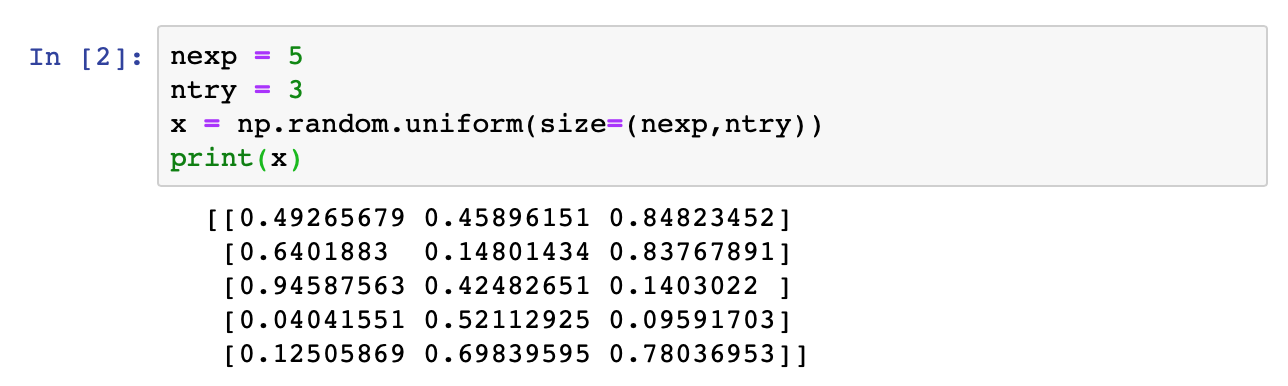
\includegraphics[width=0.85\textwidth]{figs/labs/distributions/makearray.png} \\
This array associates a random value with each trial from each
experiment.  
\item Consider a trial successful if the randomly chosen value is less
  than $\epsilon$.  In this example, taking $\epsilon = 0.5$ and
  assuming 1 indicates success and 0 a failure, we obtain:
\begin{samepage}
\begin{verbatim}
[[0 1 0]
 [0 0 1]
 [0 0 0]
 [1 1 1]
 [1 0 1]]
\end{verbatim}
\end{samepage}
In the first simulated experiment, only the second trial was
successful.  In the second experiment, only the last trial successful.
And so on.

\item Next, count the number of trials that were successful in each experiment.  The result will be a 1-D array of length $n_{\rm exp}$.  Consider using the {\tt np.sum} function with the {\tt axis} parameter (If documentation is unclear to you, check the examples).    In this example, we obtain the array of outcomes $m$:
\begin{verbatim} 
[1 1 0 3 2]
\end{verbatim}
This is the outcome of our five simulated experiments.  The first
and second experiment have one out of three trials successful, the third
experiment had zero out of three trials successful, and so on.
\end{itemize}

Work through the example and make sure you see how each result follows
from the previous step.  Then implement and test your own version of
this algorithm in Scientific Python.  If you are an experienced
programmer, you should put your simulation into a function like:
\begin{verbatim}
    def throw_binomial(nexp,ntry,eps):
       x = np.random.uniform(size=(nexp,ntry))
       #...your simulation follows...    
\end{verbatim}
This will make your code much easier to manage, because you can simply call this function each time you need to run your simulation, but it is optional.  Cutting and pasting is also permissible.


When validating a numerical calculation, think hard about good test
cases.  For instance, if you only test with the value of $\epsilon =
0.5$, you won't catch a bug that mistakes success for failure.  Try a
few different test cases, with reasonably small values for $n_{\rm
  try}$ and $n_{\rm exp}$ and check your numerical simulation.
Boundaries often make a good check, for instance $\epsilon = 0$ and
$\epsilon = 1$.

Another effective validation strategy is to check known mathematical
relations using your simulation.  For instance, we know that the mean
value of a Binomial distribution is given by:
\begin{equation} \label{eqn:binom_mean}
\bar{m} = n_{\rm try} \cdot \epsilon
\end{equation}
and that the variance is given by:
\begin{equation} \label{eqn:binom_var}
\sigma^2 = n_{\rm try} \cdot \epsilon \, (1 - \epsilon)
\end{equation}
and so these predicted values, calculated from your parameters
$\epsilon$ and $n_{\rm try}$ can be compared to the mean and variance
of the outcome array $m$ from your simulation, calculated using the numpy functions {\tt np.mean} and {\tt np.var}.  A
comparison with $n_{\rm exp}=1000$, $n_{\rm try}=10$, and
$\epsilon=0.5$ should result in something like:\\
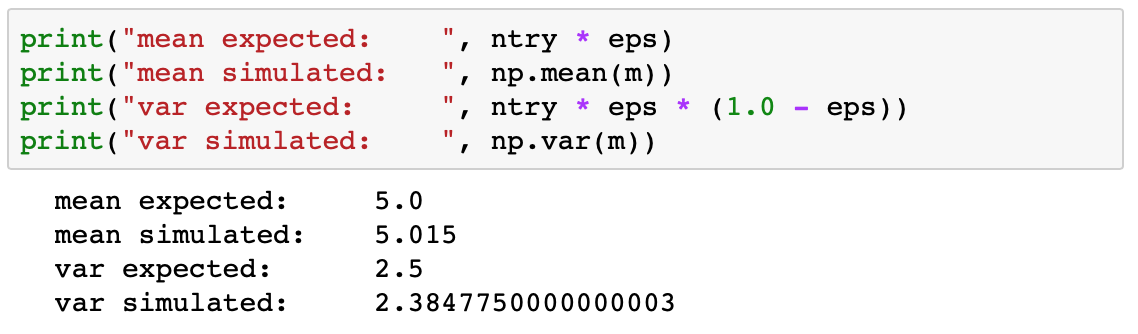
\includegraphics[width=0.8\textwidth]{figs/labs/distributions/validate.png}\\ 

\begin{print} Produce a large number of pseudo-experiments by setting $n_{\rm exp} =
1000$ and comment out any debugging print statements which will get
very long.  Pick two  well chosen test cases with different values of
$n_{\rm try}$ and $\epsilon$ and compare the expected and simulated
mean and variances. 

%Not really visual since it fluctuates and one would need to study the average behaviour for this
%Print also the values for the percent error for mean and variance
%\begin{equation}
%\mbox{percent error}= \frac{|\mbox{expected}-\mbox{simulated}|*100\%}{\mbox{expected}}
%\end{equation}

 The simulated values will fluctuate by a
fractional amount $1/\sqrt{n_{\rm exp}}$.  So for $n_{\rm exp} =
1000$, we expect the expected and simulated values to agree within
about $3\%$.  If you increase to $n_{\rm exp} = 100000$, the agreement
should improve to better than $1\%$.  Be certain to print your test
cases and the results in a clear way in your notebook. \end{print}

\section{Histogram for the Binomial Process}

We use histograms to represent the distribution of numerical data.  In
this case, our histogram simply reports the number of times each particular outcome
occurs.  Fill an output array $m$ with the simulated results of $n_{\rm exp} =
1000$ experiments each consisting of $n_{\rm try}=10$ trials with
success rate $\epsilon=0.25$.  There are eleven possible outcomes for
each of these experiments: $0,1,2,\ldots,10$.  We want to know how
often each of these outcomes occurred.

\begin{plot} Construct and plot a histogram from your simulated results in array $m$ using the 
{\tt np.histogram} function: \end{plot}
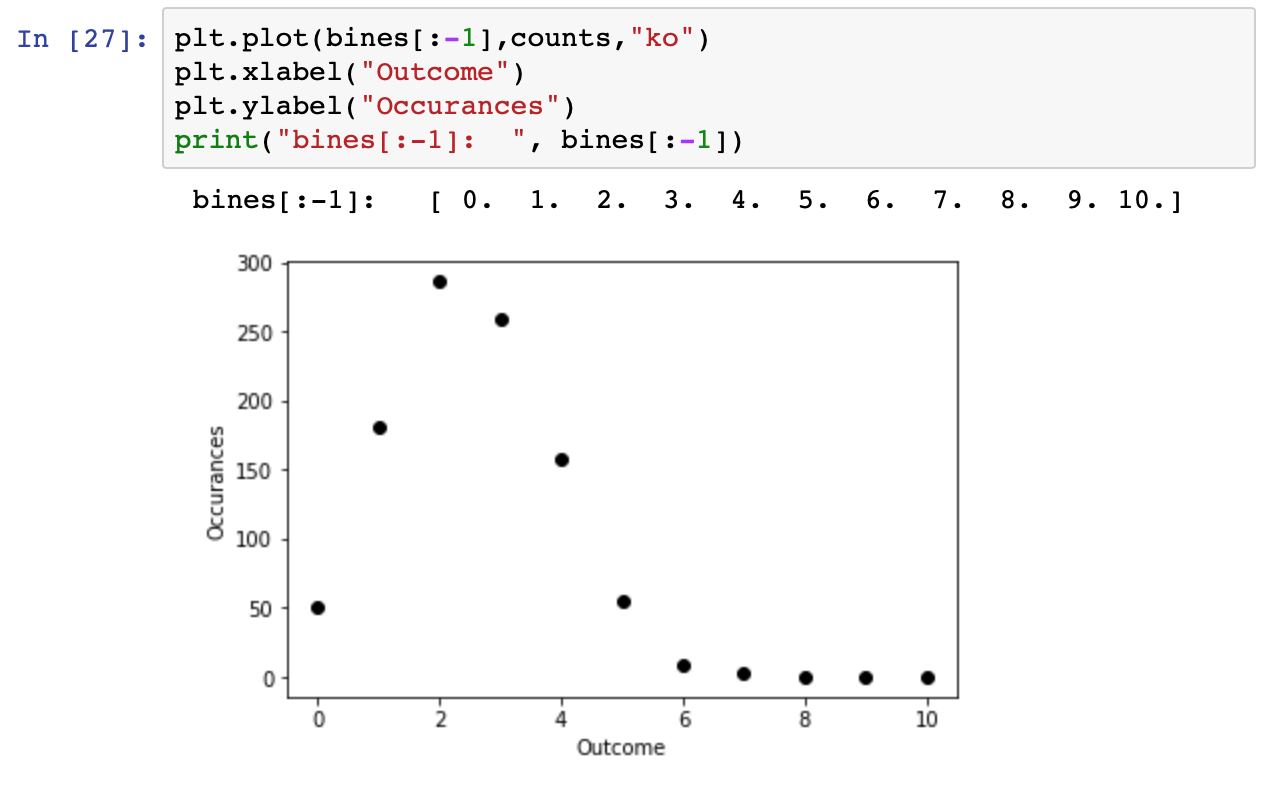
\includegraphics[width=0.8\textwidth]{figs/labs/distributions/makehist.png}\\ 
This calculates a histogram with eleven bins covering the range
from zero to eleven, and reports the number of outcomes from $m$ that
occur in each bin.  It returns two arrays, which we save as 
{\tt counts} and {\tt edges}.  We interpret the {\tt counts} array as
follows: the first entry tells us that 65 experiments had zero
successes, the second entry that 172 experiments had one success, the
third entry that 284 experiments had two successes, and so on.  The
exact values will vary each time you run the simulation, but in all
cases the sum across all bins will equal the total number of
experiments $n_{\rm exp} = 1000$.

Histograms are most often used to handle continuous data, so you
have to take a bit more care when using them to display discrete data
(integers) as we are doing here.  Consider the bin edges array {\tt
  edges} that was returned in this example:
\begin{verbatim}
   bin edges:   [ 0.  1.  2.  3.  4.  5.  6.  7.  8.  9. 10. 11.]
\end{verbatim}
which you will notice has length 12.  This is because the
array contains the {\bf edges} of eleven consecutive bins.  Technically the first bin
is the count of all outcomes in the range from zero (inclusive) to
just below one (exclusive).  The next bin is the count of all outcomes
in the range from one (inclusive) to just below two (exclusive).  In
this case, however, we are using discrete data, and so there are no entries with values like 1.73 to consider.
All the entries in the first bin are from experiments with the outcome
zero, while all the entries in the second bin are from the outcome
one.  The best way to plot this histogram, therefore, is
to associate each count with the leading bin edge, that is:\\
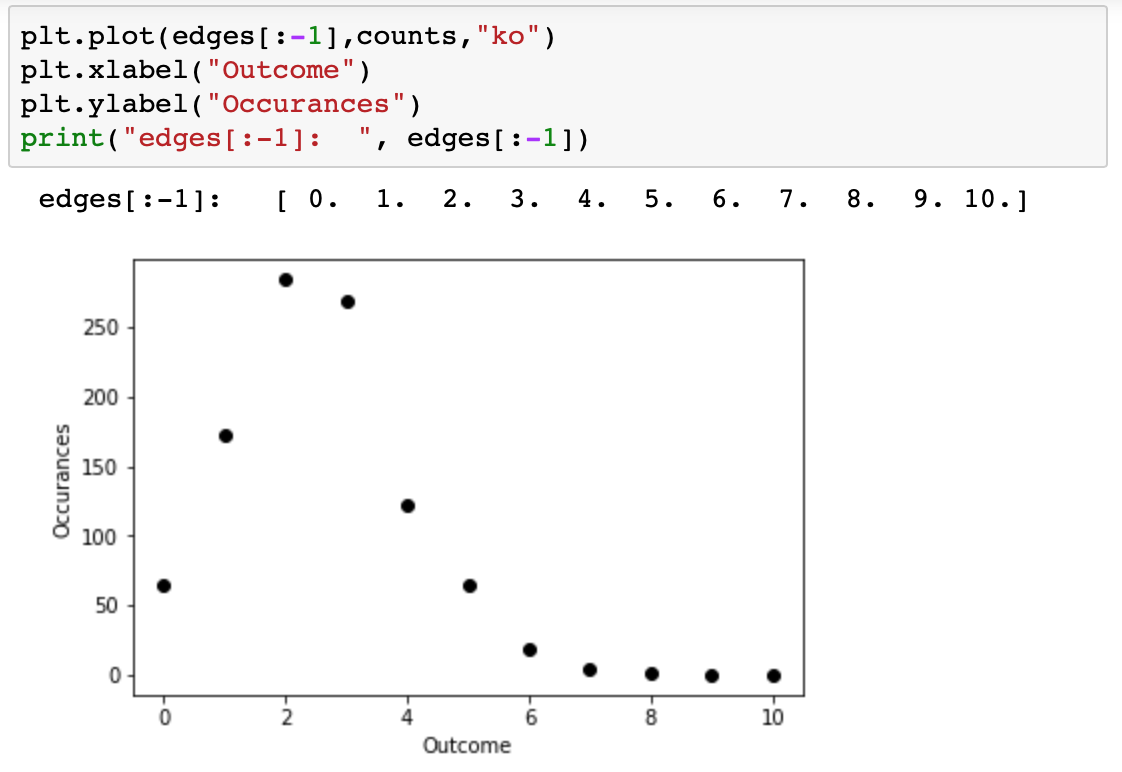
\includegraphics[width=0.8\textwidth]{figs/labs/distributions/plothist.png} \\
Notice the essential trick for plotting histogram with discrete data in integer bins is to use the slice {\tt edges[:-1]} of the bin edges data
\begin{verbatim}
   edges[:-1]:   [ 0.  1.  2.  3.  4.  5.  6.  7.  8.  9. 10.]
\end{verbatim}
as the $x$ values for plotting the occurrences of each outcome.  This
slice (all but the last entry) essentially throws out the superfluous
bin edge 11.  As we will see later, this trick only works for discrete
data in integer bins.  Notice that in resulting plot, we have the number of occurances
at each of the eleven possible outcomes correctly centered over the
numbers $0,1,2,\ldots,10.$

\section{Error Bars}

\begin{plot} Add error bars to your histogram and make a new plot.
\end{plot}
Run your simulation a few times and you will observe that the
simulated values fluctuate slightly each time you run your code.  But
how much should we expect these values to fluctuate?  If you consider
a single bin of your histogram in isolation, it contains a single
count $N$, which is itself the result of a simple counting experiment.
Counting experiments are described by the Poisson distribution.  Our
best estimate for the mean value $\lambda$ of this counting experiment
is simply our count $N$.  For the Poisson distribution the variance
$\sigma^2=\lambda$, and so we expect $\sigma = \sqrt{\lambda} =
\sqrt{N}$.  We expect each bin in our histograms to fluctuate by an
amount $\sigma$ which is the square root of the value of the bin.

To aid in interpreting histograms, it is useful to indicate the amount
we expect each bin to fluctuate by adding to the data point an ``error
bar'' with a length equal to the square root of the size of the number
of events in the
bin:\\ 
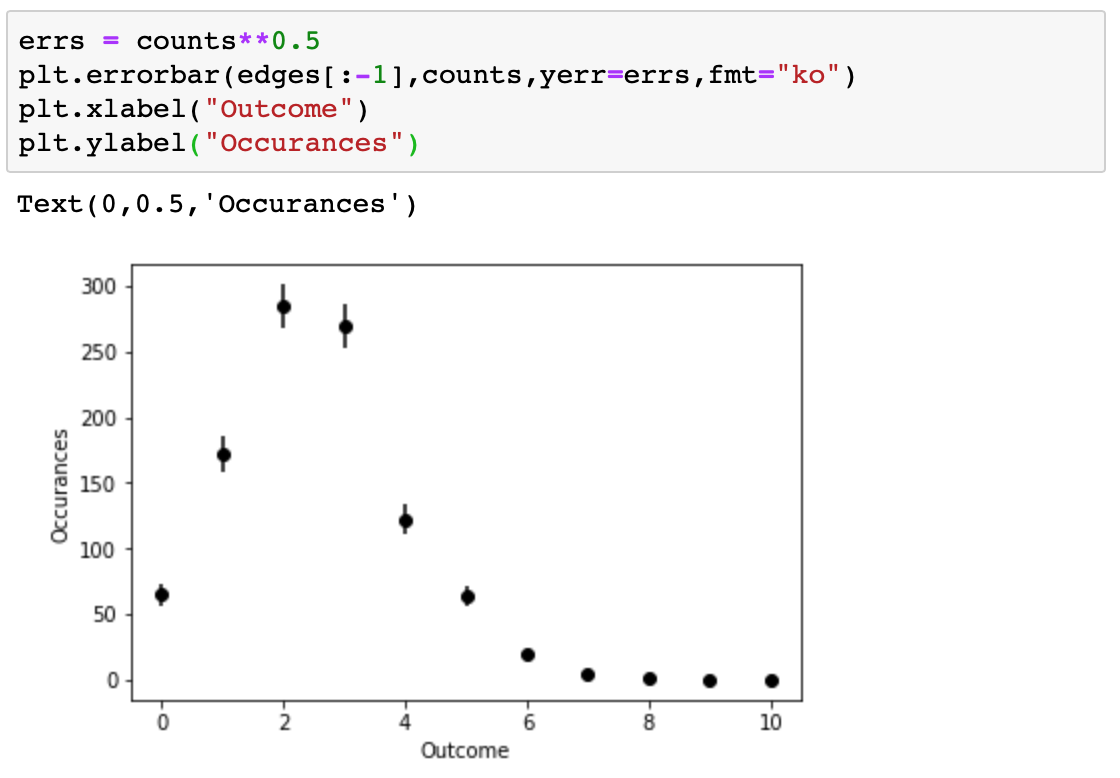
\includegraphics[width=0.8\textwidth]{figs/labs/distributions/plotbars.png}\\ 
This provides an intuitive visual indication for the size of the
statistical fluctuations associated with the counts reported by the
histogram.  Notice that the poorly named {\tt errorbar} function plots
{\em both} the data point and the error part, so it is a replacement
for the {\tt plot} function, not something you must call in addition.


\section{Comparison with Binomial PDF}

 Next we'd like to compare our Monte Carlo simulation with the PDF for
the binomial distribution.  We'll use the {\tt scipy.stats.binom.pmf}
function, which is the PDF for the discrete binomial distribution
available in Scientific Python.  This PDF is only non-zero at integer
values, so we'll simply evaluate it at each discrete occurrence,
i.e. the same slice {\tt edges[0:-1]} which we used to plot the
histogram:\\
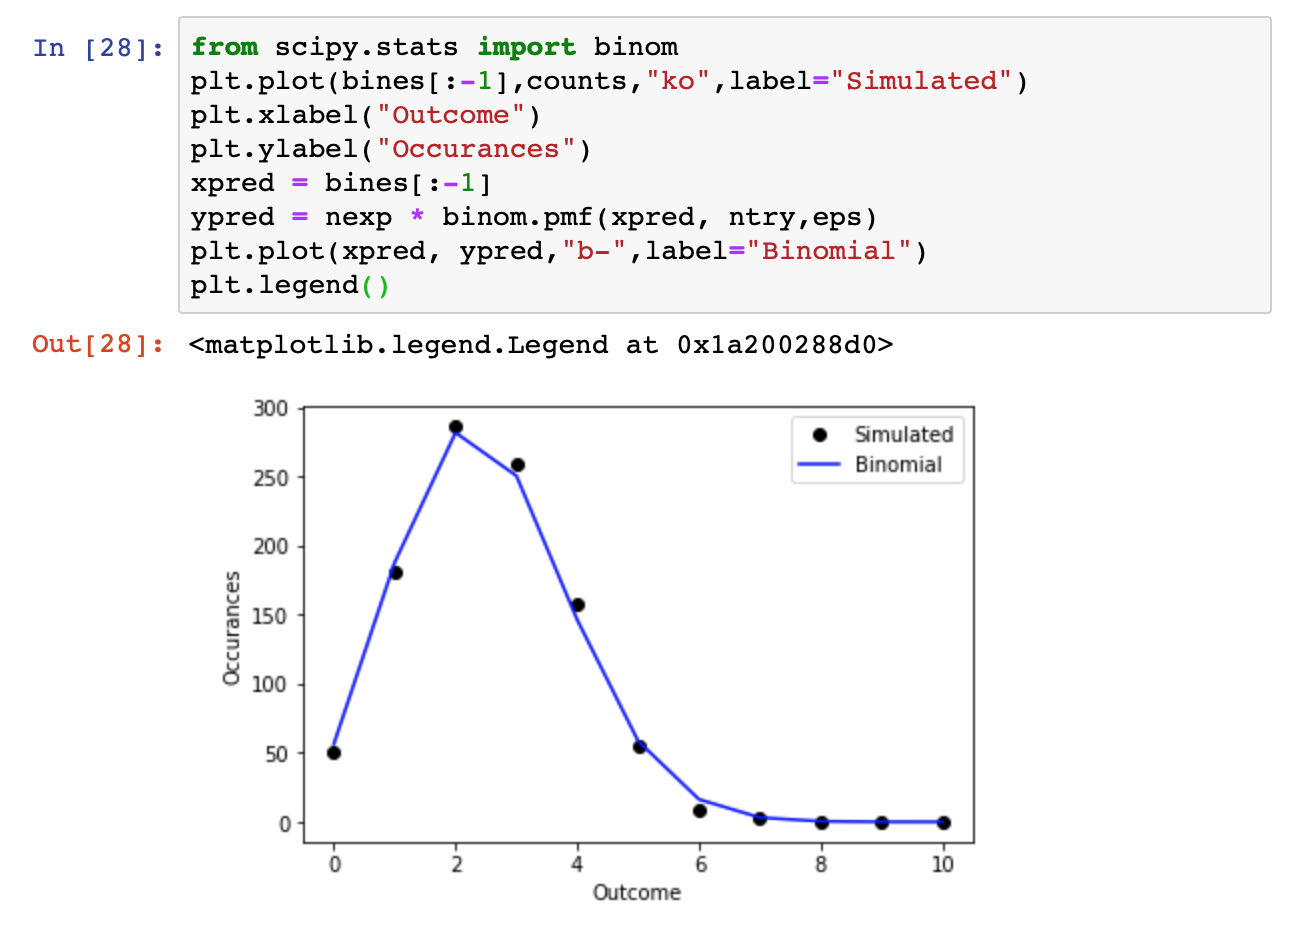
\includegraphics[width=0.85\textwidth]{figs/labs/distributions/compare.png}
\\ Notice that we scale the PDF by the number of experiments $n_{\rm
  exp}$.  The PDF is the expected frequency of each outcome for a
single experiment, but we are plotting the number of occurrences for
$n_{\rm exp}$ experiments.

\begin{plot} Compare the output of your Monte Carlo simulation
with the Binomial distribution PDF with $n_{\rm exp} = 1000$ and
$n_{\rm try} = 10$, and $\epsilon = 0.75$. See example for $\epsilon = 0.25$ in the plot above.
%and for three different values of $\epsilon$:
%0.25, 0.5, and 0.75.  For example, Plot 1 should look like the plot above. 
\end{plot}


\section{The Poisson Limit}

The Poisson distribution follows from the Binomial distribution in the
limit that $n_{\rm try} \to \infty$.  Recall that the mean value of
the Poisson distribution is $\bar{m} = \epsilon \, n_{\rm try}$.  If
we kept the success rate $\epsilon$ as a parameter, than any finite
value of $\epsilon$ would cause the mean of the distribution to diverge to infinity.
If instead we hold the new parameter $\lambda$ constant, and set:
\begin{displaymath}
\epsilon = \frac{\lambda}{n_{\rm try}}
\end{displaymath}
we see that $\epsilon \to 0$ as $n_{\rm try} \to \infty$ and the mean
of the Poisson distribution remains at the fixed value $\lambda$.

We'll explore this limit numerically simply by taking $n_{\rm try}$ to
the large (but finite) value of 1000.  Re-run your Monte Carlo
simulation using the parameters $n_{\rm try} = 1000$, $n_{\rm exp} =
1000$, and $\epsilon = \lambda / n_{\rm try}$.  For now, take $\lambda
= 2.0$.  Instead of the Binomial distribution, compare your simulation to the Poisson distribution PDF
using the {\tt poisson.pmf} function:
\begin{verbatim}
from scipy.stats import poisson
xpred = edges[:-1]
ypred = nexp * poisson.pmf(xpred, lamb) 
\end{verbatim}
Note that the first argument of the {\tt pmf} function is the array of
positions to evaluate the function at, while the second is the Poisson
parameter $\lambda$.  Also note that sadly {\tt lambda} is a reserved word
in python, and so you cannot use it as a variable name.

\begin{figure}[htbp]
\begin{center}
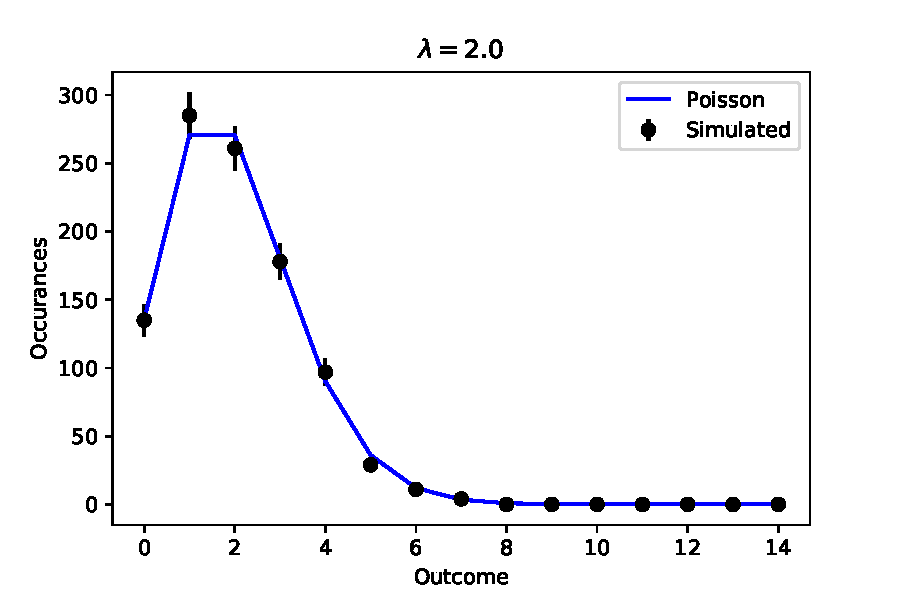
\includegraphics[height=0.22\textheight]{figs/labs/distributions/poisson.pdf}
\end{center}
\caption{\label{fig:poisson} Example of the expected result for the Monte Carlo simulation data in comparison to the Poisson PDF for for $\lambda=2$. }
\end{figure}

\begin{plot} In the Poisson limit, compare the output of your Monte Carlo simulation to the Poisson PDF
for $\lambda=5.2$.
%for two different values of $\lambda$:  2.0, 5.2.  
Plot the histogram with 15 bins for the outcomes: 0,1,2,3,...,14.  
An example for $\lambda=2$ is shown in Fig.~\ref{fig:poisson}.
\end{plot}

%Using {\tt np.mean} and {\tt np.var}, check that mean and variance of
%your distributions is as you expect in each case, and record the
%results in your log book.

This is a \textbf{sign-off point} for this lab.  Make certain you can
explain your code, and that it is as neat and organized as you can
manage.

\section{The Gaussian Limit}

\begin{figure}[htbp]
\begin{center}
\begin{tabular}{cc}
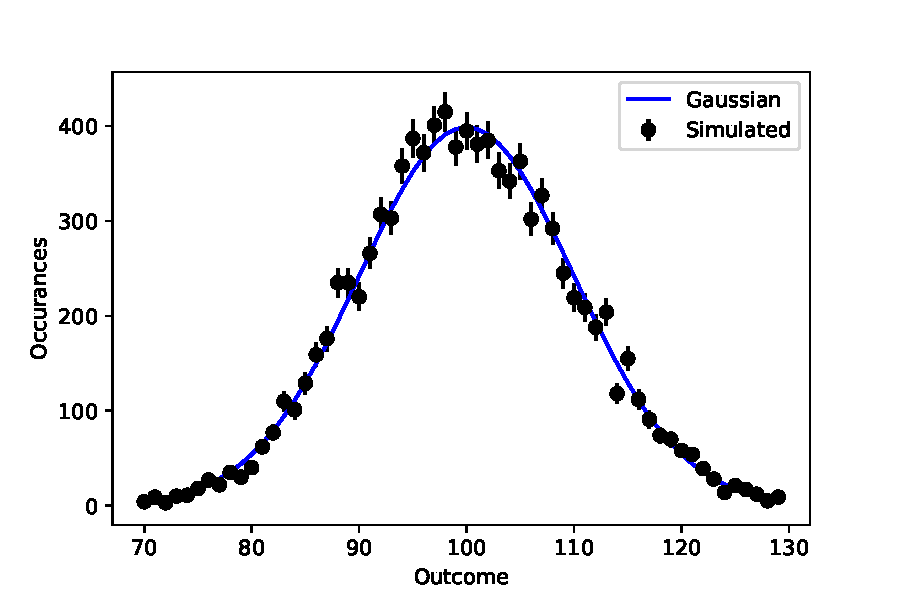
\includegraphics[height=0.22\textheight]{figs/labs/distributions/gauss_finebins.pdf} &
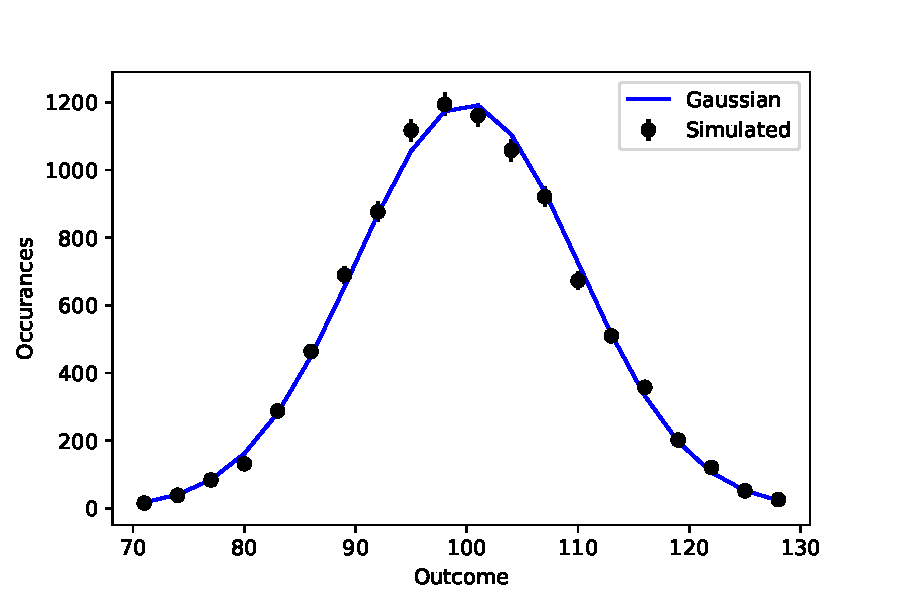
\includegraphics[height=0.22\textheight]{figs/labs/distributions/gauss.pdf} \\
(a) & (b) \\
\end{tabular}
\end{center}
\caption{\label{fig:gauss} Example of the expected result for the Monte Carlo simulation data in comparison to the Gaussian PDF for $\lambda=100$. }
\end{figure}

As the mean value $\lambda$ of the Poisson distribution gets larger,
the Poisson distribution resembles the Gaussian distribution.  We will
simulate this numerically by taking our Monte Carlo simulation in the
Poisson limit, as above, with $\lambda = 100$.  Initially use
integer bins inclusively in the range 70 to 130, e.g.:
\begin{verbatim}
counts,edges = np.histogram(m,bins=60,range=(70,130))
\end{verbatim}
and compare with the Gaussian (also called normal) distribution PDF, e.g.:
{\tt scipy.stats.norm.pdf} function:
\begin{verbatim}
from scipy.stats import norm
xpred = edges[:-1]
ypred = nexp * norm.pdf(xpred, loc=lamb, scale=lamb**0.5). 
\end{verbatim}

\begin{plot} Set the parameter {\tt loc} to the mean value, and the parameter {\tt
  scale} to $\sigma$.  Recall that in the Poisson limit $\sigma^2 =
\lambda$, which is why we set {\tt scale=lamb**0.5} in the example.
This should reproduce the plot in Fig.~\ref{fig:gauss}a. \end{plot}

You should see that 60 bins is rather unwieldy.  We'll reduce the number
of bins, but that's actually a bit more complicated than you might
expect: non-integer bins with discrete data is about the most
challenging binning you can tackle.  You'll have to do the following:
\begin{itemize}
\item While keeping the range of 70 to 130, set the number bins to {\tt bins=20} when filling your histogram.
\item Our trick to use edges[:-1] will no longer work, since now the data for each bin is associated with a range of values in the bin.  Each bin is now 3 integers wide. If we live this as is, edges[:-1] will position the x value of the bin at its leading edge: 70, 73, 76 , ......  and the data will be plotted with an observable bias.  For continuous data, we often simply use the middle of the bin:
\begin{verbatim}
cbins = (edges[:-1] + edges[1:])/2.  
\end{verbatim}
This would position the x value of the bins at 71.5, 74.5. 77.5, ..... and that seems more reasonable choice. 
In this specific case of discrete data which doesn't extend  all the way to the right edge this is still slightly biased. The first bin in our example represents the count of all outcomes in the range from 70 (inclusive) to below 73 (exclusive). So its center should be at 71.  To be precise for this specific case, the x position we should use for plotting the contents of each bin is:
\begin{verbatim}
cbins = (edges[:-1] + edges[1:] -1 )/2 
\end{verbatim}
\item The normalization of the PDF to the data now requires an additional scale factor to account for the wider bins (which integrate more probability).  You need to scale by an additional factor of 3 to account for the fact that each bin is 3 integers wide.
\end{itemize}

\begin{plot} Using the techniques described above, reproduce Fig~\ref{fig:gauss}b, which shows that the Binomial distributions becomes a Gaussian distribution as the mean value of the distribution becomes large. \end{plot}

























\chapter{Statistics of Radioactive Decays}


\section{Introduction}

\begin{figure}[htbp]
\begin{center}
 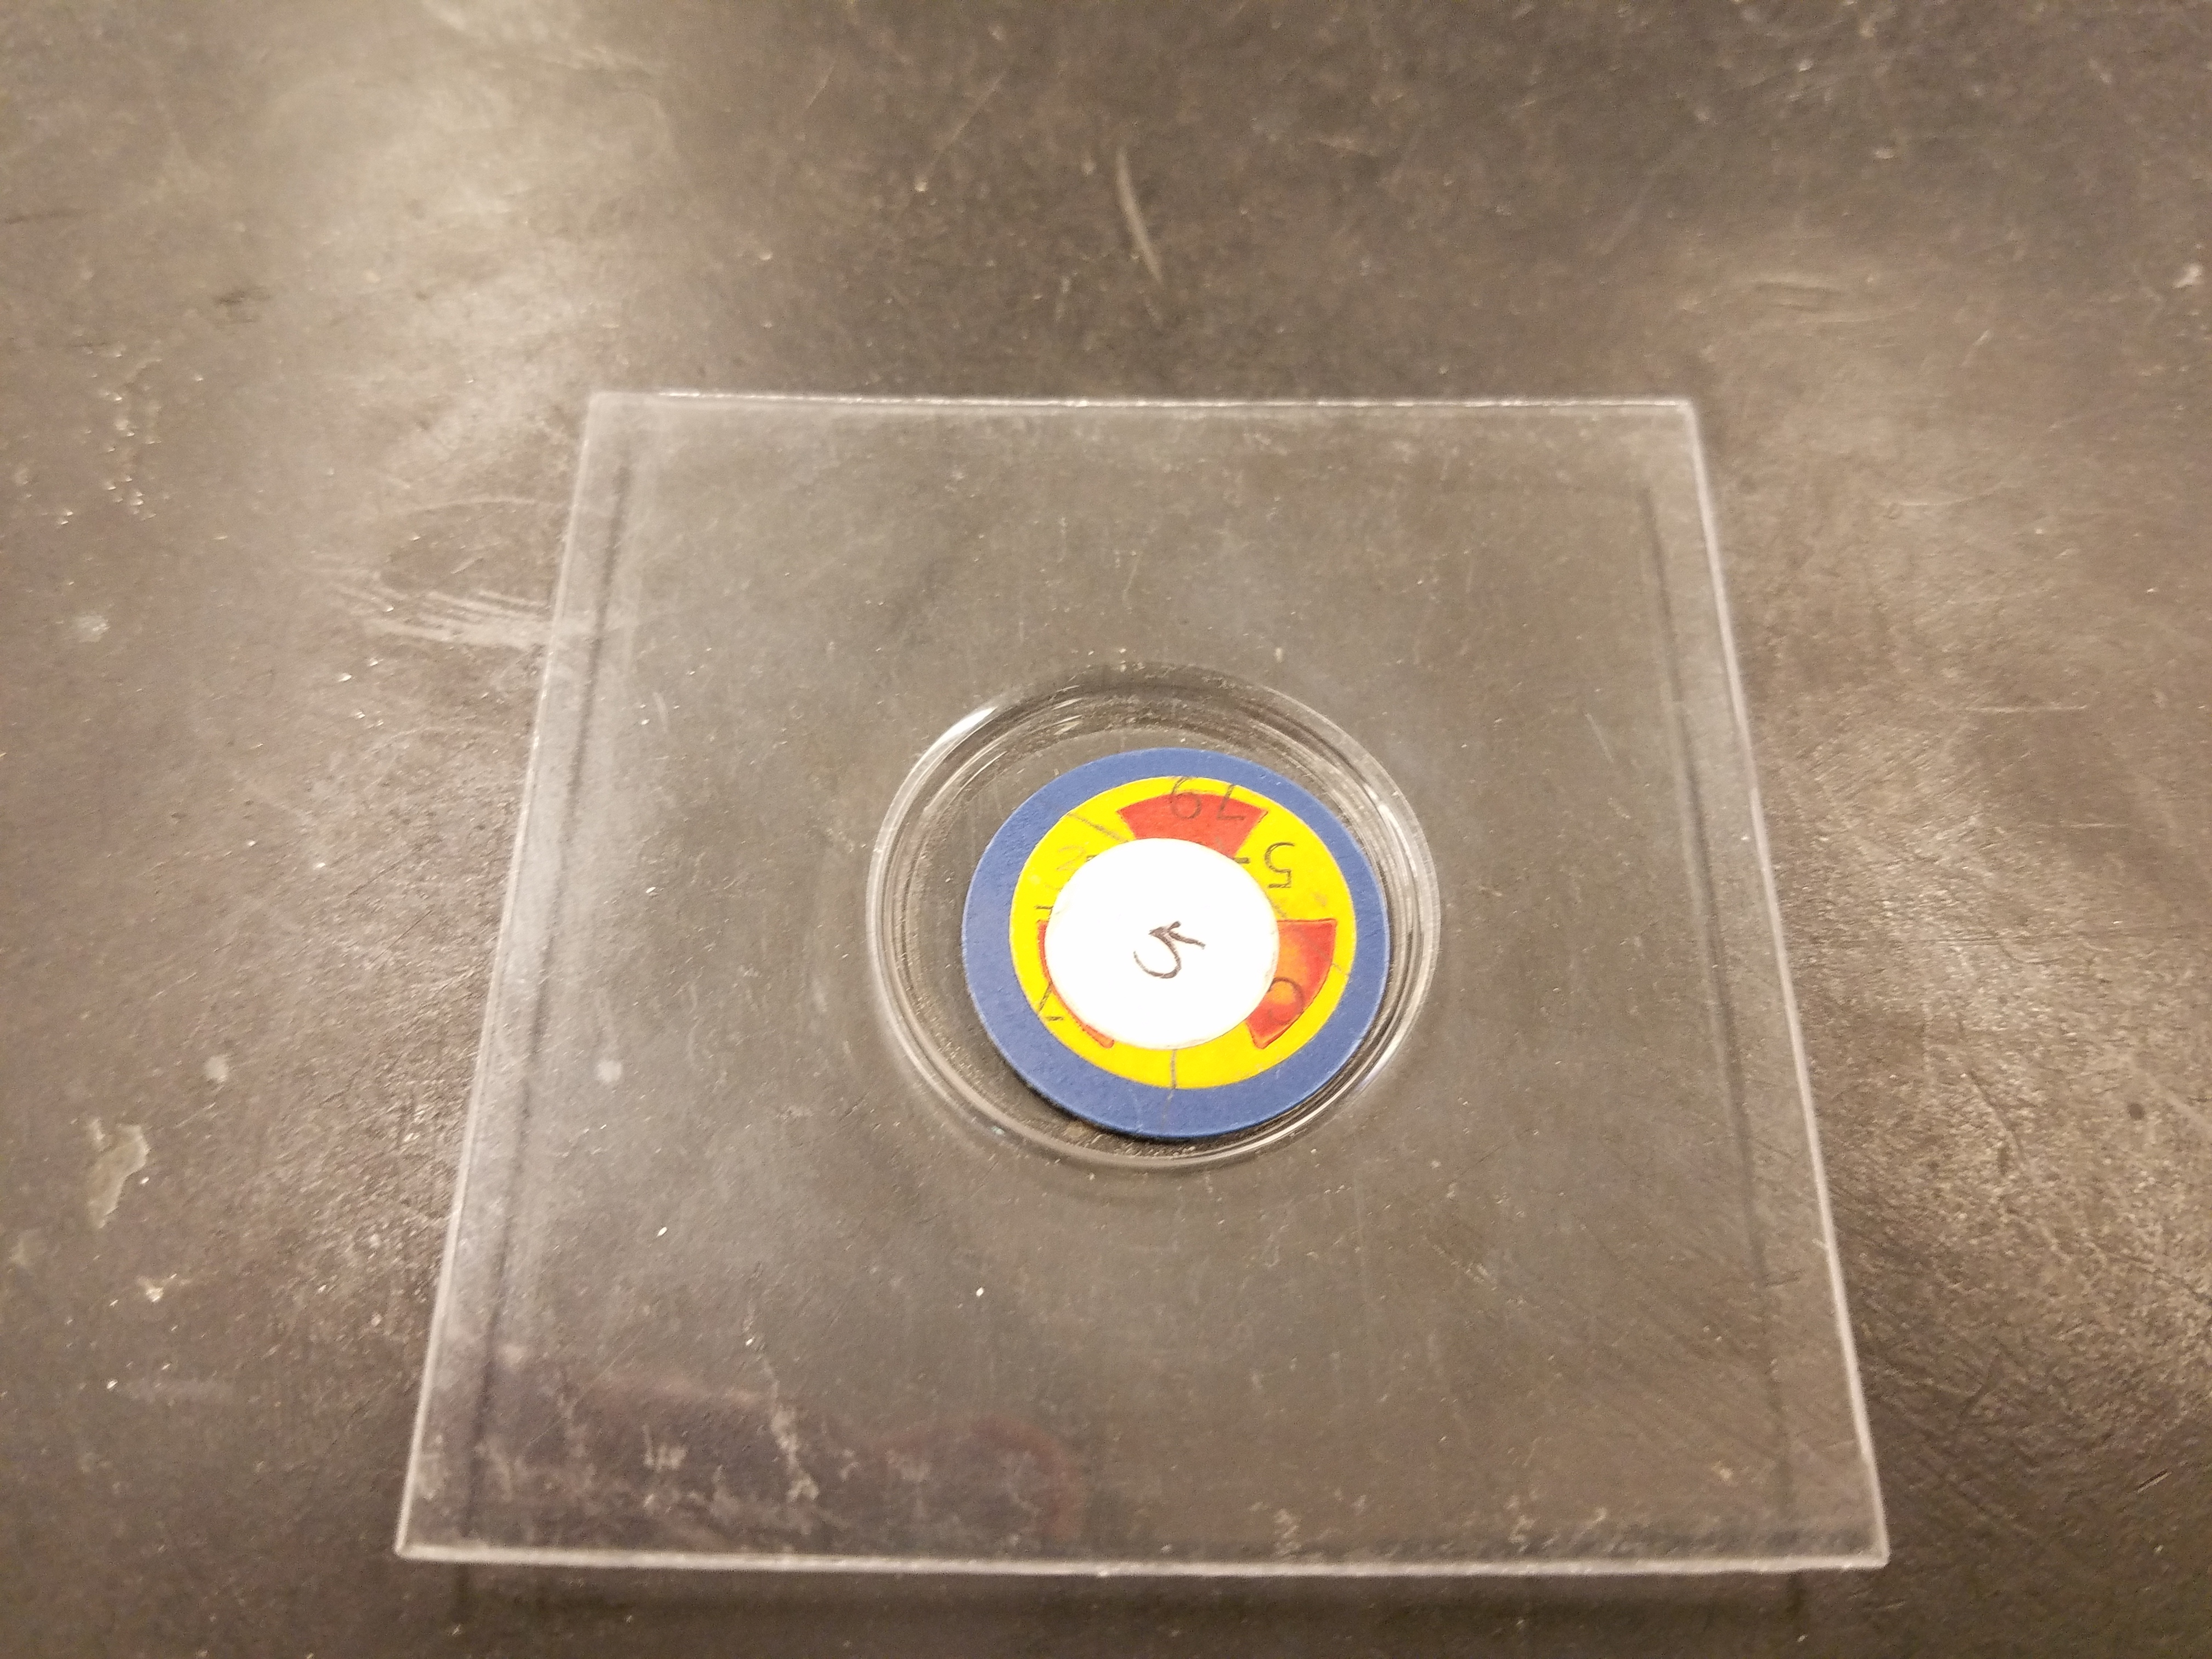
\includegraphics[width=0.55\textwidth]{figs/labs/geiger/source.jpg};
\caption{\label{fig:source} A sealed radioactive source.  A small
  amount of Cs-137 is contained within the small button shaped piece
  of plastic.  For your safety, the sources will be handled only by
  the TA.}
\end{center}
\end{figure}

In this lab, you will use a Geiger Counter to study the statistics of
radioactive decays.  For this lab there are both logbook and Jupyter
notebook entries.

\section{Precautions}

\noindent
{\bf Precautions with the Geiger counter:}
\begin{itemize}
\item Leave the cable from the Geiger counter controller to the Geiger
  counter in place {\em at all times}.  This carries voltages of
  approximately 1000 volts.  If you leave the cable in place, nothing
  can be inadvertently plugged in (including fingers).
\item Leave the Geiger tube in its holder.  It has a thin front window
  which is easily broken.
\item Do not set the high voltage higher than 1000 volts.
\end{itemize}

\noindent
{\bf Precautions with the radioactive source:}
\begin{itemize}
\item See Fig.~\ref{fig:source} to familiarize yourself with what the sources look like.
\item Don't touch the source.
\item Leave the source in the tray at all times.  The TA will provide
  the sources and handle moving them from place to place.
\item Radiation falls off as $1/r^2$.  So minimize your time near
  sources and maximize your distance from them.
\end{itemize}

\section{The Geiger Counter}

\begin{figure}[htbp]
\begin{center}
\begin{tikzpicture}
    \node[anchor=south west,inner sep=0] (image) at (0,0,0) {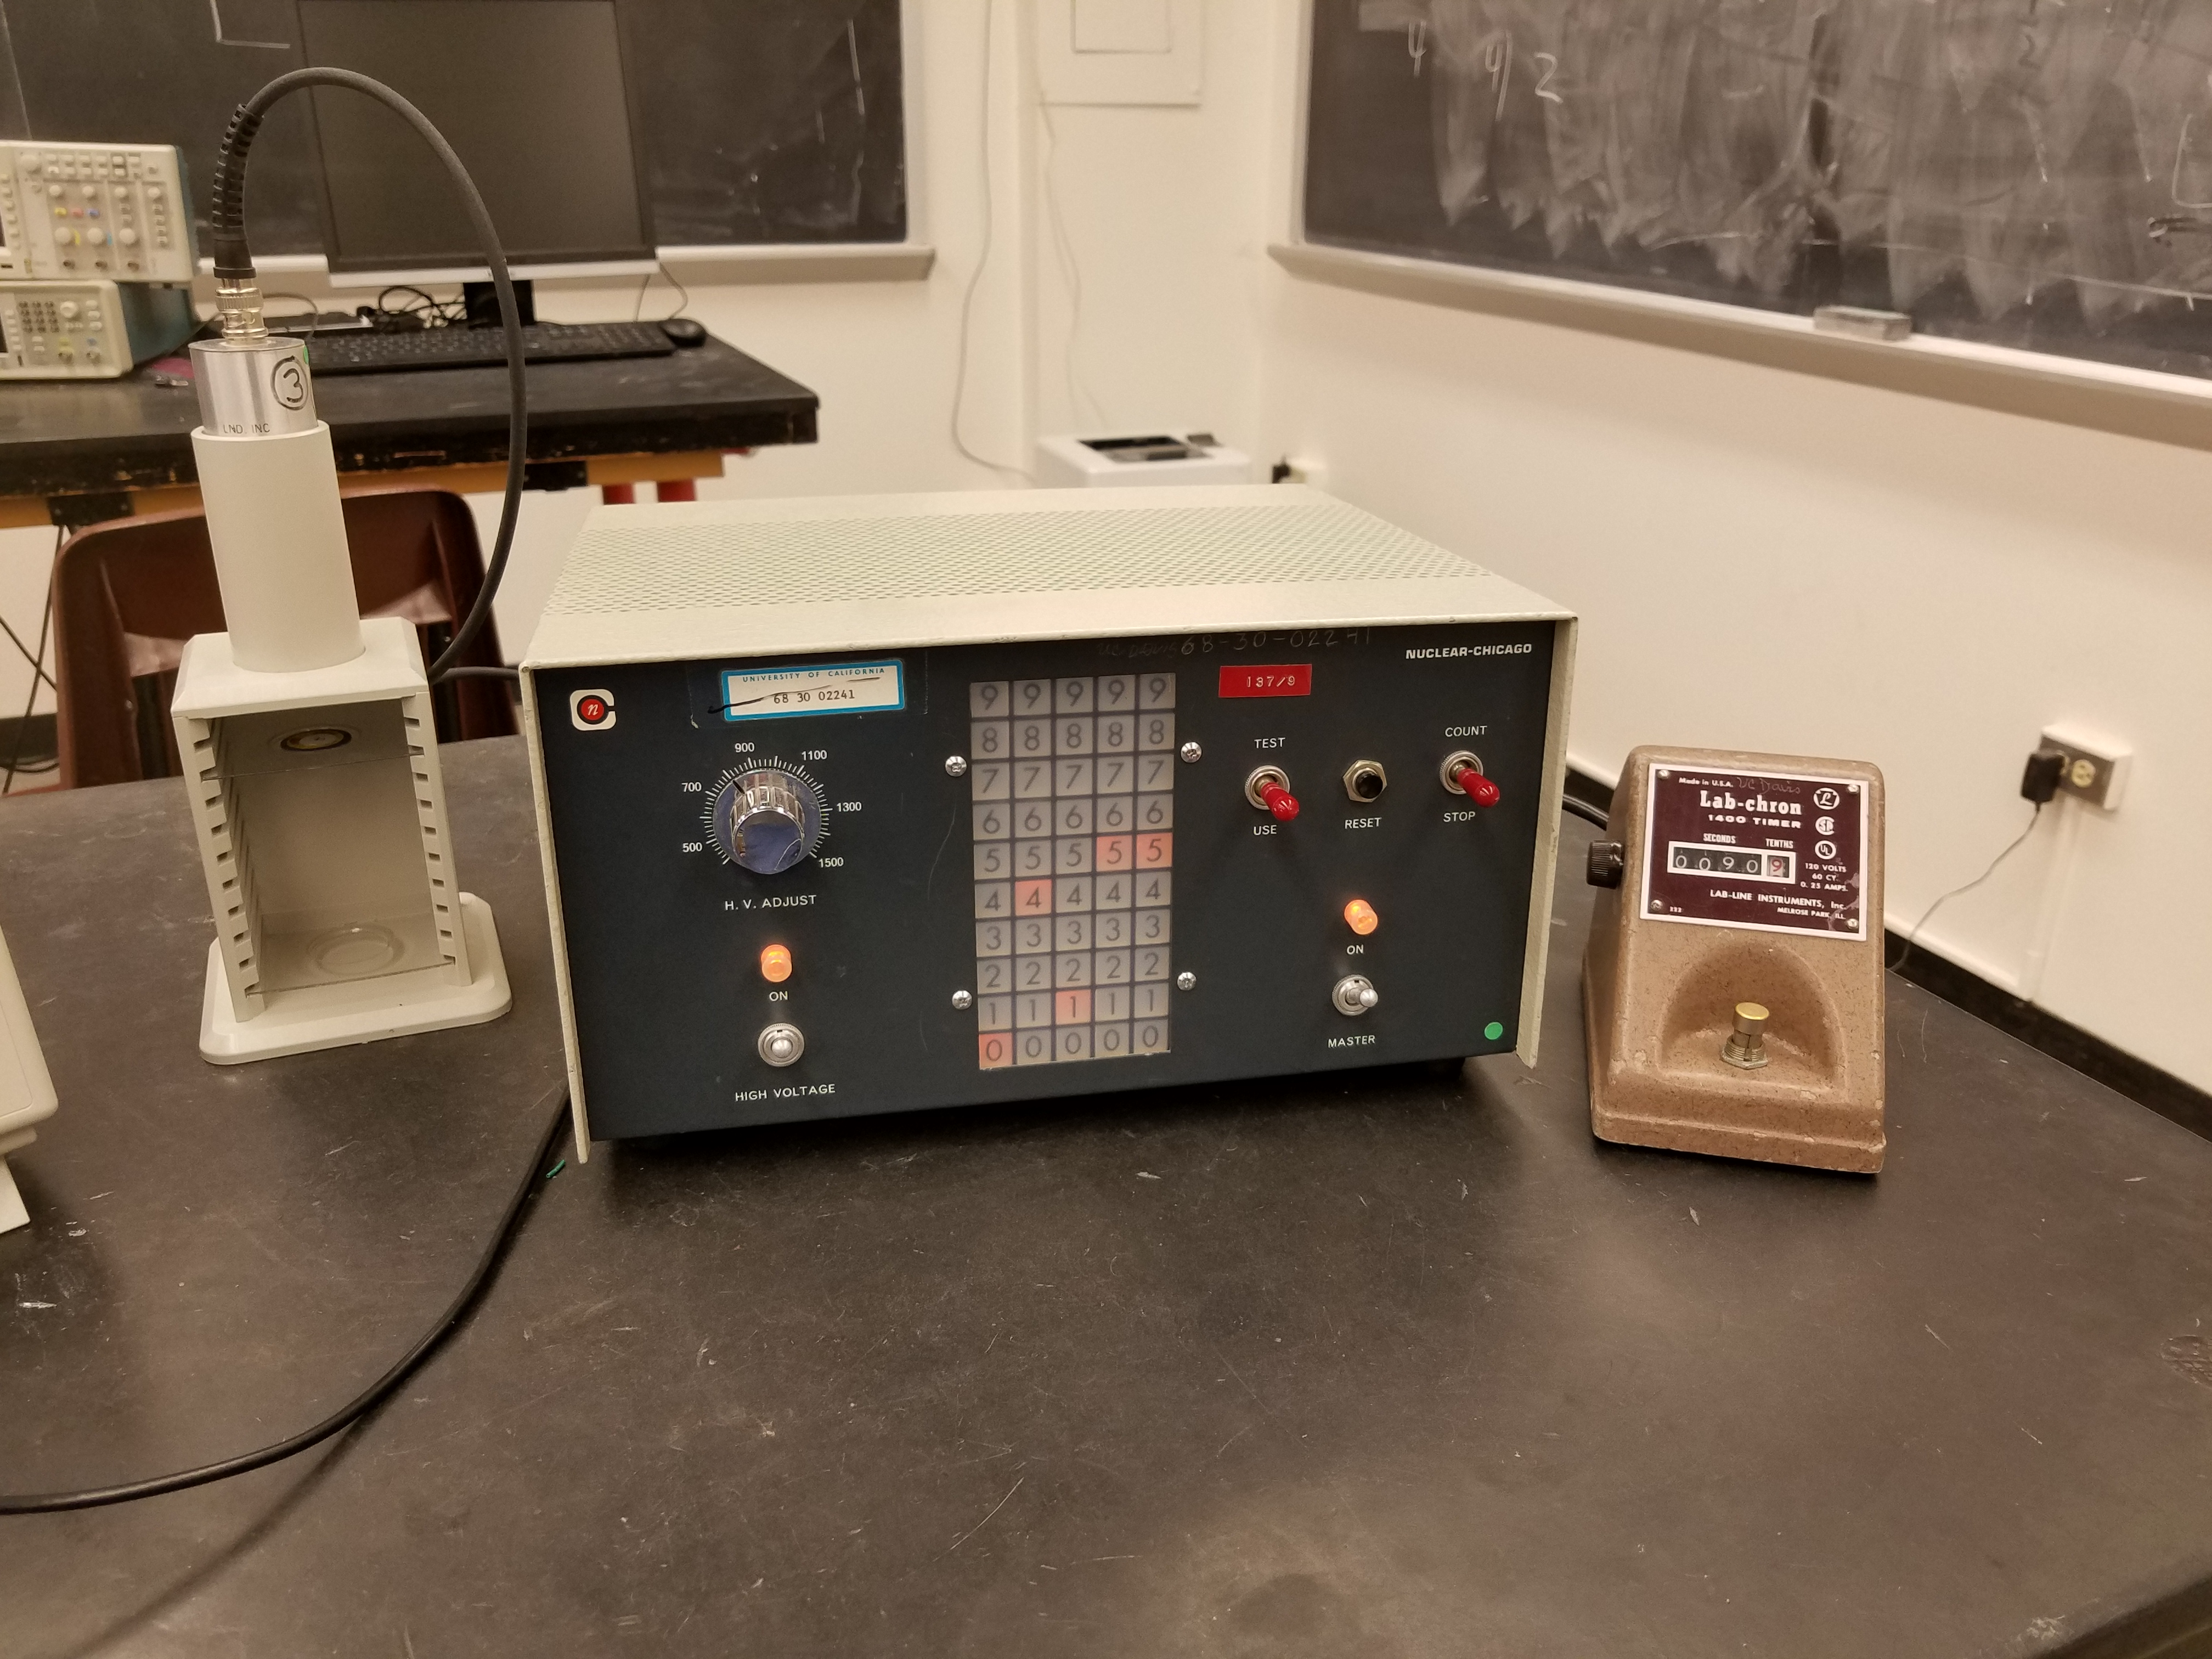
\includegraphics[width=0.55\textwidth]{figs/labs/geiger/assembly.jpg}};

    \node[right](X) at (10.0,3.0) {Timer};
    \draw (X.west) -- (8.0,3.5);

    \node[right](X) at (10.0,5.0) {\parbox{3cm}{\flushleft High-Voltage and Counter}};
    \draw (X.west) -- (5.0,4.75);

    \node[left](X) at (0.0,4.5) {\parbox{2.5cm}{\flushright Geiger Tube Holder}};
    \draw[white,thick] (X.east) -- (1.25,5.0);
    \draw (X.east) -- (1.25,5.0);

    \node[left](X) at (0.0,3.0) {Source};
    \draw (X.east) -- (1.35,4.05);

\end{tikzpicture}
\caption{\label{fig:geigersetup} The Geiger Counter assembly.}
\end{center}
\end{figure}

To begin, familiarize yourself with the counter and timer features of
your Geiger counter assembly using the built-in test mode.  Your lab
bench will already be prepared with a Geiger Counter assembly as shown
in Fig.~\ref{fig:geigersetup}.  Ensure that the high-voltage (HV) is
off by turning the knob labeled ``H.V. Adjust'' counter-clockwise all
the way to zero.  Now put the Geiger counter into test mode by
flipping the left red switch to ``TEST''.  Flip the right red switch
to ``COUNT'' and you should see the counter display begin
incrementing.  Push the button on the front of your timer and you
should see the Timer turn on and off.  Leave the timer incrementing.
Now flip right red switch to ``STOP'', and observe that the both the
counter and the timer stop simultaneously.  The knob on left side of
the old-school lab timer can be used to reset the time.  Keep turning
the knob clockwise until the time reads 0.  Use the black button on
the Counter to reset the count to zero.

Flip the right switch to ``COUNT'' and then back to ``STOP'' when 10
seconds have passed.  During this time, the $60~\rm Hz$ test signal
should increment the counter close to 600 times.  Try this a few times
and make sure you can reliably count close to $600$ test pulses in a
10 second interval.  You should reset the count each time, but there
is no need to reset the timer.  Simply stop when the timer reaches the
next factor of ten.  Due to your reaction time, you may well stop at
one-to-two tenths of a second later.  This is OK, and will only add
less than a few percent error to your measurements over 10 second
intervals.

\section{High-Voltage Calibration}

When you are confident that you know how to operate the timer, switch
the left red switch to ``USE'' mode.  Unless a sealed radioactive
source is already in place, ask the TA to provide you with a source in
the second shelf from the top of your Geiger tube holder.  Switch the
right switch to ``COUNT'' mode.  With the HV off, you should not see
any pulses.  Turn the HV up until you begin to see counts increment on
the display, and continue to the next interval of 50 volts (e.g. if it
first starts incrementing at 730 volts, set the dial to 750 volts).
Count the number of events in a ten second interval.

Repeat this measurement in 50 volt steps up to 1000 volts.  Do not exceed 1000 volts.

\begin{plot}
Plot the rate (in Hz) as a function of high voltage.  You should see a
plateau region (a leveling off) which indicates the onset of the
Geiger mode within the Geiger tube.  The Geiger tube has some
resistance even in Geiger mode, so do not expect a perfectly flat
plateau.  From your plot, chose a high-voltage near the beginning of
the Geiger mode, and set the high-voltage to this calibrated value.
If you are struggling with Python, you can make a rough plot by hand
in your logbook to determine the plateau region, and leave the fancy
plot for later.
\end{plot}

\begin{figure}[htbp]
\begin{center}
 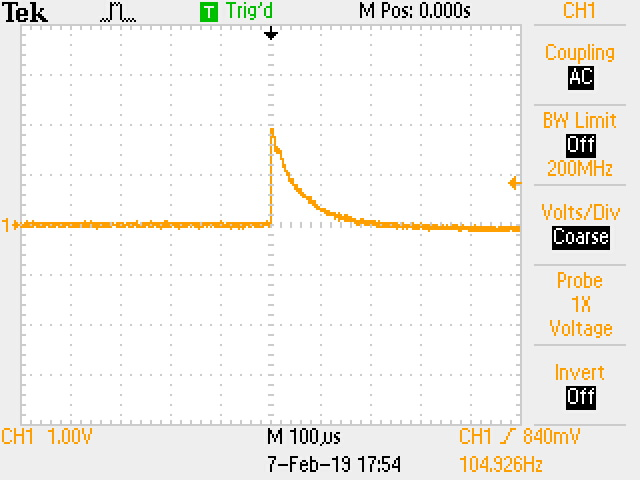
\includegraphics[width=0.55\textwidth]{figs/labs/geiger/pulse.jpg};
\caption{\label{fig:geigerpulse} An example Geiger counter pulse.}
\end{center}
\end{figure}

Connect an oscilloscope to the output of the counter assembly (on the
back, labeled ``SCOPE'').  Adjust your scope to view the Geiger pulses
like that of Fig.~\ref{fig:geigerpulse}.  Note that the Geiger counter
output contains a DC component in addition to the AC pulse, so you
will want to use your scope in AC coupling mode which will remove the
DC component and allow you to see the pulse.  You will also want to
see the attenuation to 1X because you are not using an attenuating
probe.

\begin{measurement}
Sketch a typical Geiger counter pulse in your logbook and indicates the pulse height and time duration.
\end{measurement}

\section{Data Collection}

Even in today's world of digital automation, it is still useful to
know how to collect a small amount (up to a few hundred data points)
of data manually.  Often in the lab, you have one-off measurements
that you would like to make without investing in automation.

In this section, you will collect data manually for about one hour.
Practice a routine with your lab partner that allows you to take and
record the data as fast as possible.  For instance, person A should
operate the counter, and person B should use the PC.  Person A turns
the counter on for ten seconds, turns it off, and says (quietly)
``OK''.  Person B records the value on the PC and says ``Go''.  Person
A resets the counter and continues.  Remember that there is no need to
reset the Timer each time, which would take too long, and which would
actually be counterproductive (if you consider the effect of a roughly
constant reaction time.) 

Practice your routine a few times, and make sure your count is near
1000 events in a ten second interval.  Then record 120 data points.

When you have finished recording your data with the radioactive
source, ask your TA to remove the source and return it to the
radioactive locker.

Now record an additional 120 data points with no source, to measure
the background radiation rate.  You should record around 3 background
counts per 10 second interval.

\section{Analysis}

\begin{figure}[htbp]
\begin{center}
\begin{tabular}{cc}
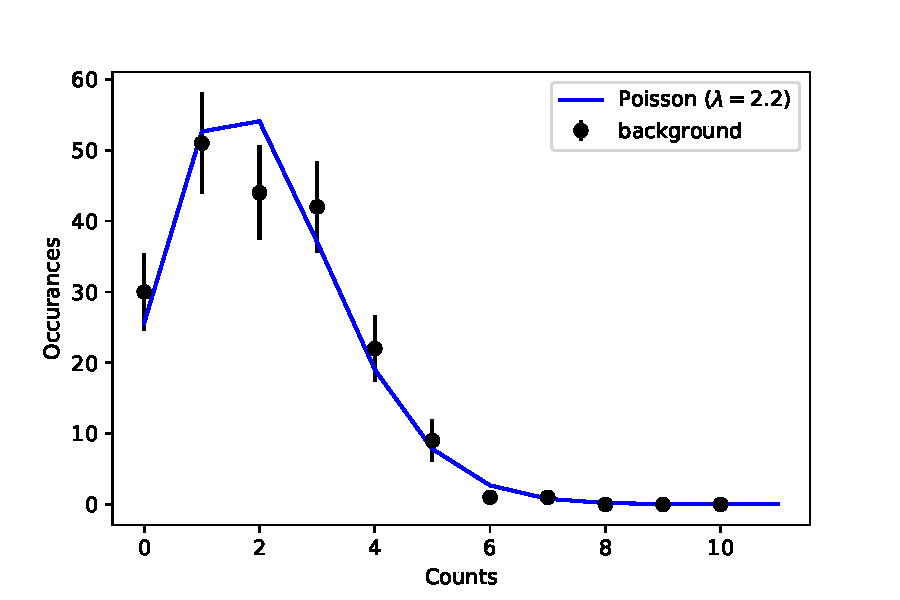
\includegraphics[height=0.22\textheight]{figs/labs/geiger/background.pdf}
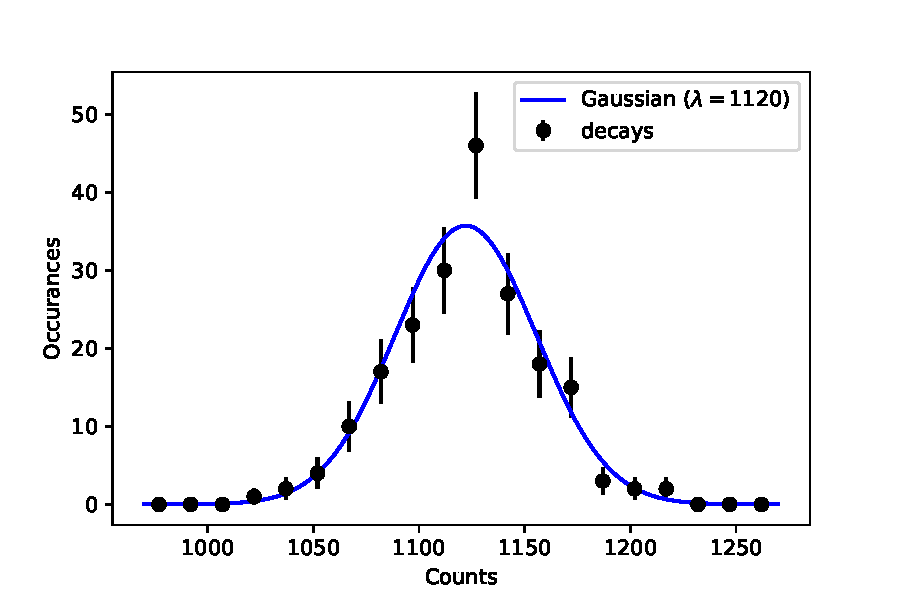
\includegraphics[height=0.22\textheight]{figs/labs/geiger/source.pdf}
\end{tabular}
\end{center}
\caption{\label{fig:geigeranalysis} Numerical simulation of the experiment
  for (a) background radiation only, and (b) radioactive source
  present.}
\end{figure}

Using Scientific Python, measure the mean and variance of your
collected background and source data.  Then produce histograms to
display your data as in Fig.~\ref{fig:geigeranalysis}.  For the
background data, plot the histogram for eleven bins: 0,1,2,...,10.
For the source data, plot about 20 bins covering a few hundred counts
around the mean value.

\begin{plot} Compare your collected background data to a Poisson distribution,
appropriately normalized, with a mean set to the mean of your data. \end{plot}
\begin{plot} Compare your collected source data to a Gaussian distribution,
appropriately normalized, with a mean set to the mean value of your
data, and sigma set to the square root of your mean. \end{plot}

This is a \textbf{sign-off point} for this lab. 
%move this earlier have them take data with source and analyze then sign off point plus data taking for only background plus analysis; so if they are late they get some plots that could be discussed.









\chapter{The Central Limit Theorem and Experimental Uncertainties}

%
% TODO:  Students were confused about how to handle bin position
% for plotting discrete data...  some clarification (text, figures) is needed.
%

\section{Introduction}

In this lab, you will produce a numerical demonstration of the central
limit theorem.  You will also model the propagation of uncertainties
and compare with the calculated uncertainties. For this lab there are only jupyter notebook entries. 


\section{Sampling Distributions}

\begin{figure}[htbp]
\begin{center}
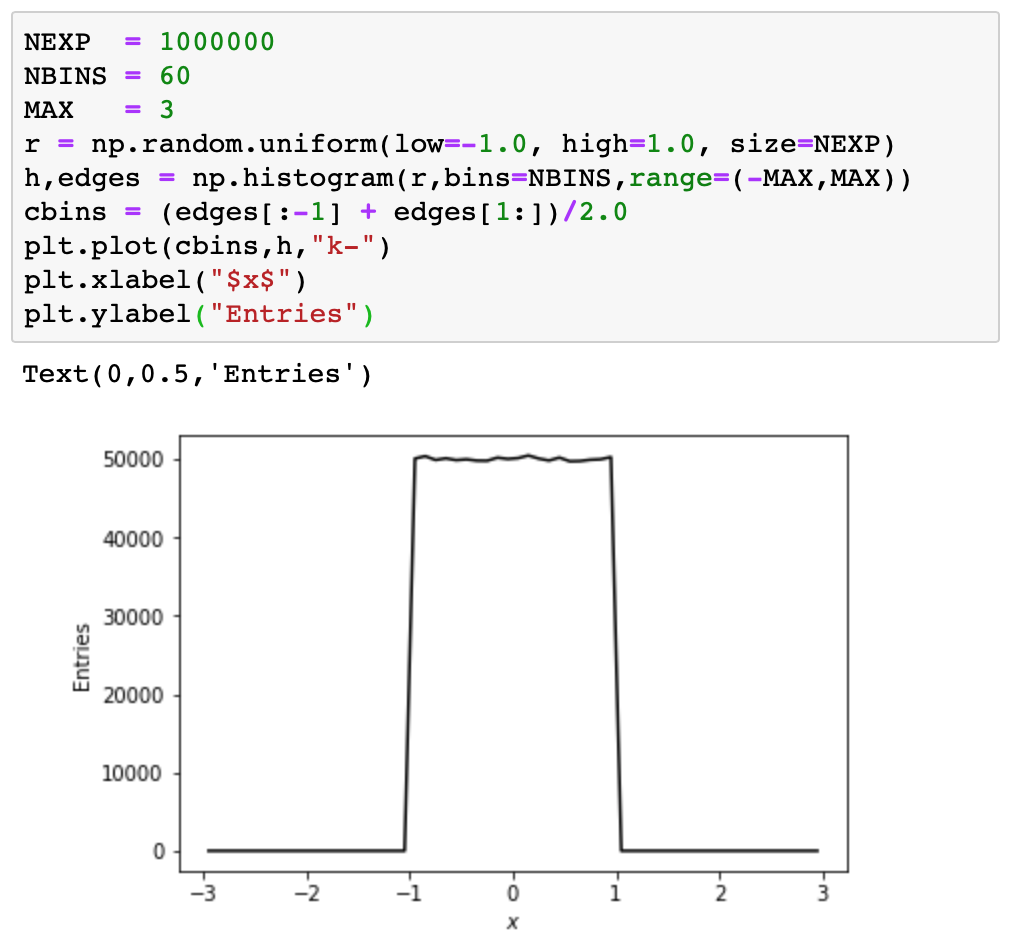
\includegraphics[width=0.75\textwidth]{figs/labs/uncertainties/step.png}\\
\end{center}
\caption{\label{fig:samplingstep} Sampling from the uniform distribution. }
\end{figure}

\begin{figure}[htbp]
\begin{center}
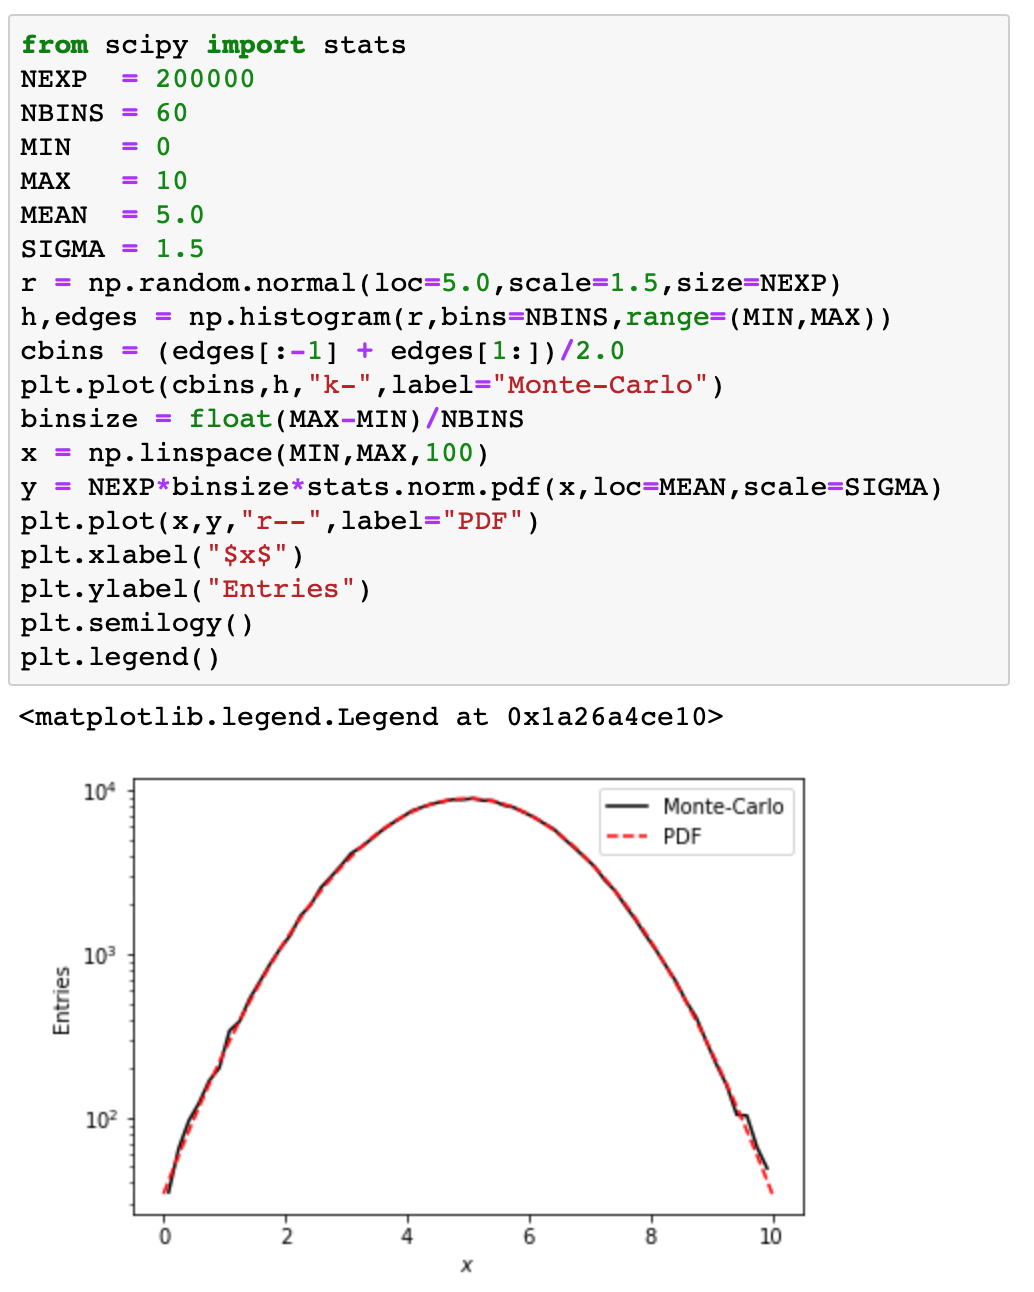
\includegraphics[width=0.75\textwidth]{figs/labs/uncertainties/gaussian.png}\\ 
\end{center}
\caption{\label{fig:samplinggauss} Sampling from the Gaussian distribution and comparison with the Gaussian PDF.}
\end{figure}

Scientific python provides functions to draw random samples according
to various distributions.  In today's lab, we will draw samples
uniformly in the interval $[-1,1]$, as demonstrated in Fig.~\ref{fig:samplingstep}.   The line
\begin{verbatim}
r = np.random.uniform(low=-1.0, high=1.0, size=NEXP)
\end{verbatim}
creates a NumPy array {\tt r} which contains {\tt NEXP} entries, with
each entry chosen uniformly and randomly in the range from -1 to 1.
In the example, these events are displayed in a histogram.  When
plotting histograms with plenty of statistics (one million entries
here) and fine binning (60 bins here) it is usually preferable to use
lines instead of points with error bars for plotting the histograms,
as is done in this example.  Notice, however, that even with one
million events, there are still statistical fluctuations which prevent
the curve from being perfectly smooth.

In Fig.~\ref{fig:samplinggauss}, entries are instead drawn from the Gaussian distribution with the line:
\begin{verbatim}
r = np.random.normal(loc=5.0,scale=1.5,size=NEXP).
\end{verbatim}
The histogram is plotted with a logarithmic $y$ scale:
\begin{verbatim}
plt.semilogy()
\end{verbatim}
which results in the Gaussian distribution appearing as a parabola.  The histogram is compared to the Gaussian PDF appropriately normalized:
\begin{verbatim}
x = np.linspace(MIN,MAX,100)
y = NEXP*binsize*stats.norm.pdf(x,loc=MEAN,scale=SIGMA)
\end{verbatim}


\section{Demonstration of the Central Limit Theorem}

In this section, you'll show that average value of random variables
chosen uniformly from -1 to 1 approaches a Gaussian distribution,
consistent with the central limit theorem.  First create a 2-D array
of size {\tt NEXP} by {\tt NAVG} filled with uniform random values in
the interval from -1 to 1, as follows:
\begin{verbatim}
r = np.random.uniform(low=-1.0, high=1.0, size=(NEXP,NAVG))
\end{verbatim}
Then calculate averages values from {\tt NAVG} entries:
\begin{verbatim}
x = np.sum(r, axis=1)/float(NAVG)  
\end{verbatim}
From the Central Limit Theorem, we expect the entries in x to approach a Gaussian distribution.

\begin{plot}  Set {\tt NEXP} to 1000000 for plenty of statistics.
Produce three different histograms with 40 bins covering the range
from -1.2 to 1.2 for three values {\tt NAVG}: 1,2, and 3.  Plot all
three histogram in the same graph with appropriate legend. \end{plot}

Your plot will show that already for three contributions to the average, the result looks quite Gaussian on a linear scale.  For more precise comparison, will use a log scale and compare to the PDF.

\begin{plot} Calculate {\tt NEXP}$=1000000$ average values {\tt x} for {\tt NAVG}$=10$.  Calculate the mean value of the entries in {\tt x} using the {\tt np.mean} function.  Calculate $\sigma$ for the entries in $x$ by taking the square root of the output from the {\tt np.var} (variance) function.  Produce a histograms with 20 bins covering the range
from -0.5 to 0.5 for the average values.  Compare with a Gaussian distribution, appropriately normalized, using your calculated values from the  mean and sigma.  Plot both the histogram and PDF on the same graph, including an appropriate legend.  Use a logarithmic $y$ axis. \end{plot}


\section{Propagation of Uncertainties}

\begin{figure}[htbp]
\begin{center}
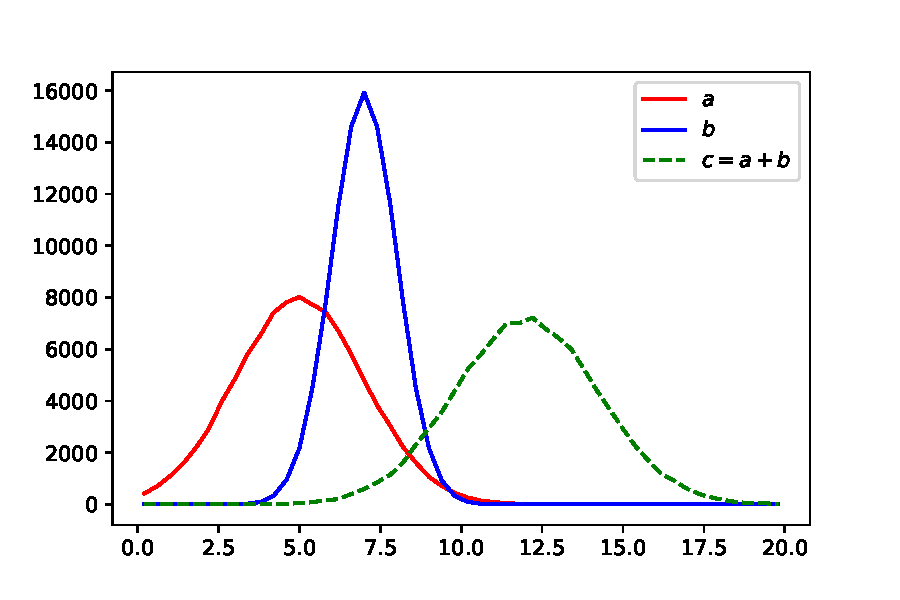
\includegraphics[width=0.75\textwidth]{figs/labs/uncertainties/addunc.pdf}\\
\end{center}
\caption{\label{fig:addunc} Simulation of many measurements of the quantity $c = a + b$. }
\end{figure}

Consider two measured values $a \pm \sigma_a$ and $b \pm \sigma_b$.  If we calculate the quantity $c = a + b$ or $c = a - b$, the uncertainty on the calculated value $c$ is given by:
\begin{displaymath}
\sigma_c = \sqrt{\sigma_a^2 + \sigma_b^2}.
\end{displaymath}
If instead, we calculate $c = a * b$ or $c = a/b$ the fractional uncertainty on $c$ is given by:
\begin{displaymath}
\frac{\sigma_c}{c} = \sqrt{\left(\frac{\sigma_a}{a}\right)^2 + \left(\frac{\sigma_b}{b}\right)^2}.
\end{displaymath}
In this section, you'll develop a numerical simulation for the
propagation of uncertainties under addition, subtraction,
multiplication, and division.  An example, for $c = a + b$ is shown in Fig.~\ref{fig:addunc}.

\begin{print} Pick values for $a$, $b$, $ \sigma_a$ and $ \sigma_b$ for simulating subtraction: $c=a-b$. Print them out in your notebook. Choose the values that are different from what is plotted in Fig.~\ref{fig:addunc}.  \end{print}

\begin{plot} 
Simulate the measurement $a$ by drawing 100,000 random variables
sampled from the Gaussian distribution with mean $a$ and sigma
$\sigma_a$, and likewise for $b$.  Calculate the values of $c = a -b $ from
the $a$ and $b$ values.  Plot the result in histogram with 50 bins and an appropriate range. \end{plot} 

\begin{print} 
Calculate the mean and variance of the mean and variance of the simulated $c$ values and compare to your expectations for the mean, variance of the distribution and variance of the mean. Apply the standard propagation of uncertainties for calculating expectation value for the variances. 
 \end{print}


This is a \textbf{sign-off point} for this lab. 

\begin{print} Pick values for $a$, $b$, $ \sigma_a$ and $ \sigma_b$ for simulating division: $c=a/b$. Print them out in your notebook.  Choose the values that are different from what is plotted in Fig.~\ref{fig:addunc}.  \end{print}

\begin{plot} 
Simulate the measurement $a$ by drawing 100,000 random variables
sampled from the Gaussian distribution with mean $a$ and sigma
$\sigma_a$, and likewise for $b$.  Calculate the values of $c = a/b $ from
the $a$ and $b$ values.  Plot the result in histogram with 50 bins and an appropriate range. \end{plot} 

\begin{print} 
Calculate the mean and variance of the mean and variance of the simulated $c$ values and compare to your expectations for the mean, variance of the distribution and variance of the mean. Apply the standard propagation of uncertainties for calculating expectation value for the variances. 
 \end{print}

 
%{\bf Plot 3-6:}  Produce four plots simulating addition, subtraction, multiplication, and division, as in Fig.~\ref{fig:addunc}.  In each case, compare the measured variance of the $c$ values with your expectation.































\chapter{The Diode}

\section{Pre-lab Calculations}
\noindent
1) Suppose a diode is in forward bias with a resistor $R=10~k\Omega$ in series while connected to a $10~\rm V$ DC source.  Estimate the effective resistance of the diode.  Hint: assume a typical diode drop of $0.6~\rm V$ and consider an equivalent voltage divider consisting entirely of resistors. \\ 

\noindent
2) Consider the circuit in Fig.~\ref{fig:diodecircuits}a and assume $R_1=1.8~\rm k \Omega$ and the peak-to-peak voltage is $V_{\rm pp} = 5~\rm V$.  What is the peak current through the diode?  The math is easier if you assume a diode drop of $0.7~V$, so go ahead and do so! \\

\noindent
3) What is the ripple current for an AC source with amplitude $10~\rm V$ and frequency $100~\rm Hz$ driving a load of $R_L=18~\rm k\Omega$ in the circuit in Fig.~\ref{fig:fwrectc} for (A) $C=1~\mu F$ and (B) $C=100~\mu F$?

\section{Introduction}

In this lab, you will measure the IV curve of a diode, use it to predict the operating point of a circuit, and use rectification to provide a DC current source with low ripple voltage.   In the process, you will learn how to use the Math mode of your scope to make a differential voltage measurement.

\section{Measuring the $I$-$V$ Curve of a Diode}

In this section you will measure the $I$-$V$ curve of a 1N914 diode, and compare your results to the curves available from the device data sheet.  To avoid taking a bunch of measurements by hand, we will use a trick to plot the curve directly on your oscilloscope using the XY mode.
\begin{figure}[htbp]
\begin{center}
\begin{tabular}{c@{\hskip 2cm}c}

\begin{circuitikz}[line width=1pt]
\draw
(0,0) to[sinusoidal voltage source,bipoles/length=1.5cm,l=$\tilde{V}$] (0,4) -- (2,4);
\draw
(2,4) node[right]{$P_2$} to[resistor,l=$R_1$,o-o] (2,2) node[right] {$P_1$} to[diode,l=$D_1$,-o](2,0) node[right]{G}-- (0,0)
;
\draw (0,0) -- ++(0,0) node[ground,yscale=2.0]{};
\end{circuitikz} &

\begin{circuitikz}[line width=1pt]
\draw
(0,0) to[sinusoidal voltage source,bipoles/length=1.5cm,l=$\tilde{V}$] (0,4) -- (4,4);
\draw
(2,4) to[resistor,l_=$R_1$,*-o] (2,2) node[left]{$P_1$} node[right]{(Ch.1)} to[diode,l_=$D_1$,o-*] (2,0)
(4,4) to[diode,l=$D_2$,-o] (4,2) node[right] {$P_2$ (Ch.2)} to[resistor,l=$R_2$,-o](4,0) node[right]{G}-- (0,0)
;
\draw (2,0) -- ++(0,0) node[ground,yscale=2.0]{};
\end{circuitikz} \\
(a) & (b) \\
\end{tabular}
\caption{Diode circuits for (a) demonstrating rectification and (b) plotting the diode IV curve on your oscilloscope.}
\label{fig:diodecircuits}
\end{center}
\end{figure}

Consider (but don't build!) the circuit in Fig.~\ref{fig:diodecircuits}a.  The voltage between points $P_2$ and $P_1$ is proportional to the current passing through the diode, and the voltage between points $P_1$ and $G$ is the voltage across the diode.  So if we could display $P_2-P_1$ versus $P_1-G$ on your scope we could use this circuit.  Unfortunately, this is not possible on your scope, because (1) the only valid place to put the scope probe ground shield clips is at the point $G$ (Why?) and (2) you can only display Channel 1 versus Channel 2 in XY mode.   

The solution is to drive two copies of the diode in series resistor, with the component order reversed, as in Fig.~\ref{fig:diodecircuits}b.  This way, we can connect the probe ground shields as required at point $G$, put the voltage across the diode on scope Channel 1 by connecting the probe tip at $P_1$, and put the voltage across the resistor (proportional to current through the diode) on scope Channel 2 by connecting the probe tip at $P_2$.

Build the circuit in Fig.~\ref{fig:diodecircuits}b using a 1N914 fast switching diode for $D_1$ and $D_2$ and $R_1= R_2 = 10~{\rm k\Omega}$.  Set your function generator for high-impedance output, providing AC with peak to peak voltage of $20~\rm V$ at a frequency of $100~\rm Hz$.  Before switching to XY mode, make certain that your Channel 1 has no voltage offset (that is, zero voltage is located at the origin) or else your diode output voltage won't be calibrated properly in your output plot.   Once you set this, try not to adjust the offset of Channel 1 or you'll have to redo it!  To minimize noise, set the bandwidth limit ``On'' for both channels (this is available in the menu for each input channel as ``BW Limit'').

\begin{figure}[htbp]
\begin{center}
\begin{tabular}{c@{\hskip 2cm}c}
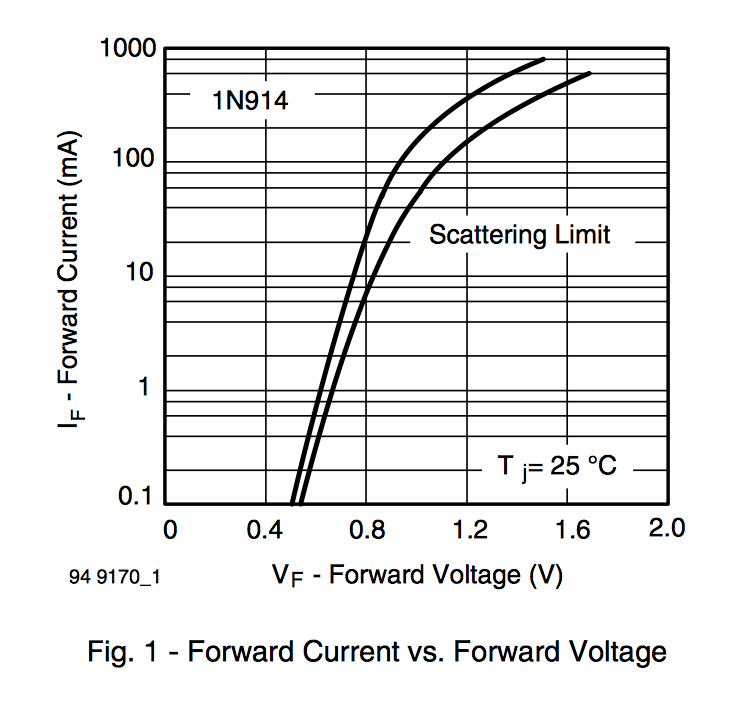
\includegraphics[height=0.25\textheight]{figs/labs/diode/1N914.png} &
\begin{picture}(200,100)
\put(0,0){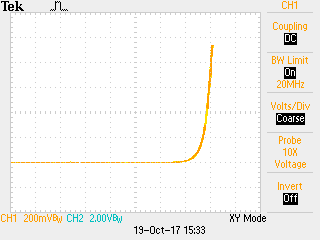
\includegraphics[height=0.25\textheight]{figs/labs/diode/diodeiv.png}}
\put(10,52){$0~mA$}
\put(10,70){$0.2~mA$}
\put(10,88){$0.4~mA$}
\put(10,106){$0.6~mA$}
\put(10,124){$0.8~mA$}
\put(10,142){$1.0~mA$}
\end{picture}\\
(a) & (b) \\
\end{tabular}
\caption{\label{fig:diodeiv} IV curves for the1N914 from (a) data sheet, and (b) as you will measure in this lab.  In the scope trace, the Channel 2 ($Y$) with scale set to $2~\rm V$ measures the voltage across a $10~\rm k\Omega$ resistor, so each division corresponds to $200~\rm \mu A$ as indicated. 
}
\end{center}
\end{figure}

Set the scope into XY mode, and see if you can reproduce the diode IV curve in Fig~\ref{fig:diodeiv}b.
Beats jotting down voltages in your logbook doesn't it?  Now jot down the voltage you expect across the diode for a current of $1~\rm mA$ in your logbook.  Where they overlap, does your measured IV curve agree with the curve from the component data sheet in Fig.~\ref{fig:diodeiv}a?

\section{Rectifying an AC Signal}

\begin{figure}[htbp]
\begin{center}
\begin{circuitikz}[line width=1pt]
\draw
(0,0) to[sinusoidal voltage source,bipoles/length=1.5cm,l=$\tilde{V}$] (0,4) -- (2,4)
(2,4) node[right]{$P_2$} to[diode,l=$D$,o-o] (2,2) node[right] {$P_1$} to[resistor,l=$R$,-o](2,0) node[right]{$G$} -- (0,0)
(2,0) -- ++(0,0) node[ground,yscale=2.0]{};
\end{circuitikz} 
\caption{A diode rectification circuit.}
\label{fig:rect}
\end{center}
\end{figure}

Set your function generator to provide an AC source with frequency $100~\rm Hz$ and peak-to-peak voltage $V_{\rm pp}=5~\rm V$.  Build the circuit in Fig.~\ref{fig:rect} using a 1N914 diode for $D$ and $R=1.8~\rm k\Omega$. 

With your scope probe ground shield clips both properly connected to the ground at $G$, monitor the voltage at points $P_1$ and $P_2$.   Sketch the voltage across the resistor $R$ and the voltage supplied by the function generator versus time on the same plot in your lab book. 

Using your scopes amplitude measurement feature, measure precisely (i.e. to within $50~\rm mV$ precision) the voltage drop across the diode at the peak current value, by measuring the difference between Channel 1 and Channel 2 of your scope at the peak.  Is this operating point consistent with your results from the previous section and the pre-lab calculations?

\section{Building a DC voltage source}

Now build the DC source circuit in Fig.~\ref{fig:fwrect} using a 1N914 diode for $D$ and $R_{\rm L}=18~\rm k\Omega$.  Adjust your function generator to provide a peak-to-peak voltage $V_{\rm pp} = 20~\rm V$.   

\begin{figure}[htbp]
\begin{center}
\begin{circuitikz}[line width=1pt]
\draw
(4,0) -- (0,0) node[left]{$G$} to[sinusoidal voltage source,l=$\tilde{V}$,bipoles/length=1.5cm,o-] (0,4) -- (4,4)
(2,2) to[diode,l_=D,-*] ++(0,-2) 
(2,2) to[diode,l=D,-*] ++(0,2) 
(4,4) to[diode,l_=D] ++(0,-2) 
(4,0) to[diode,l=D] ++(0,2)
(2,1.8) to[short,*-] ++(4,0) -- ++(0,-1.8) -- ++(2,0) coordinate (A)
(4,2.2) to[short,*-] ++(2,0) -- ++(0,1.8) -- ++(2,0) coordinate (B)
(B) -- ++(0,-1) coordinate (C)
(A) -- ++(0,1) node[right]{$P_1$} to[R,l=$R_{\rm L}$,o-o] (C) node[right]{$P_2$}
(2,0) -- ++(0,0) node[ground,yscale=2.0]{}
;
\end{circuitikz}
\caption{A full-wave rectifier.  Note that crossed lines without a dot are {\em not connected.}}
\label{fig:fwrect}
\end{center}
\end{figure}

To measure the performance of our DC source, we would like to measure the voltage across the resistor $R_L$ on the scope.  However, notice that the ground for the circuit is located at point $G$, so you cannot measure the voltage between $P_1$ and $P_2$ using a single probe.  To make the measurement, connect  both probe ground shield clips to the point $G$ as required, and connect the probe tips to points $P_1$ and $P_2$.  Next, use your scope's Math mode to subtract Channel 1 to from Channel 2.  The result of this operation is the voltage across the resistor $R_{\rm L}$.

Sketch the current as a function of time for a few cycles, and measure the amplitude.  In your lab report, explain the shape and the amplitude.

\section{Controlling the Ripple}

In class, we derived the following formula for the ripple voltage (the residual AC voltage after rectification) 
for a full-wave rectifier with a capacitance $C$:
\begin{displaymath}
\Delta V = \frac{I_{\rm max}}{2 f C}
\end{displaymath}
Add a capacitor with $C=1~\rm{\mu F}$ to your circuit, as in Fig.~\ref{fig:fwrectc} and sketch the resulting waveform for the voltage across the load resistor as measured with your scope.  Estimate the ripple voltage.  As your DMM is a handheld device that is not DC coupled, you may use it to measure the voltage across $R_L$ directly.  Using your DMM, measure the voltage across $R_L$ in both AC and DC mode.   How does the AC measurement relate to the ripple voltage $\Delta V$?  How do you various measurements compare to the voltages you calculated in pre-lab calculations?

For the last tweak, you are going to use a large electrolytic capacitor.  {\bf These capacitors are polarized, and will likely ``let the smoke out'' if you install them the wrong way.}  Making sure the negative terminal is connected as indicated in Fig.~\ref{fig:fwrectc}, install a $C=100~\rm \mu F$ electrolytic capacitor in your circuit and measure the ripple voltage.

\begin{figure}[htbp]
\begin{center}
\begin{circuitikz}[line width=1pt]
\draw
(4,0) -- (0,0) node[left]{$G$} to[sinusoidal voltage source,l=$\tilde{V}$,bipoles/length=1.5cm,o-] (0,4) -- (4,4)
(2,2) to[diode,l_=D,-*] ++(0,-2) 
(2,2) to[diode,l=D,-*] ++(0,2) 
(4,4) to[diode,l_=D] ++(0,-2) 
(4,0) to[diode,l=D] ++(0,2)
(2,1.8) to[short,*-] ++(4,0) -- ++(0,-1.8) -- ++(2,0) coordinate (D)
(4,2.2) to[short,*-] ++(2,0) -- ++(0,1.8) -- ++(2,0) coordinate (E)
(D) to[pC,l=$C$] (E)
(D) to[short,*-] ++(2,0) coordinate (A)
(E) to[short,*-] ++(2,0) coordinate (B)
(B) -- ++(0,-1) coordinate (C)
(A) -- ++(0,1) node[right]{$P_1$} to[R,l=$R_{\rm L}$,o-o] (C) node[right]{$P_2$}
(2,0) -- ++(0,0) node[ground,yscale=2.0]{}
;
\end{circuitikz}
\caption{A full-wave rectifier with ripple voltage limiting capacitor.  When using a polarized electrolytic capacitor, make certain that the negative terminal is connected to the lower half of the figure, as indicated.
}
\label{fig:fwrectc}
\end{center}
\end{figure}

\section{Lab Report}

Your report should include all of your measurements and a comparison with your calculation.
 


\chapter{Curve Fitting}
%ADD CHI2 calculation 
\section{Introduction}

In this lab, you will learn about curve fitting with Scientific Python
function {\tt curve{\_}fit}.  For this lab there are only jupyter notebook entries. 

Given a function to fit $f(x;p)$, with p
representing any number of parameters, and a set of measurements $y_i$ and points $x_i$,
the {\tt curve{\_}fit} function determines the best fit parameters by
minimizing:
\begin{equation}
\chi^2 = \sum_i \frac{(f(x_i;p) - y_i) ^2}{\sigma_i^2}.
\label{eqn:chi2}
\end{equation}
If the uncertainties $\sigma_i$ are not specified, the function
assumes $\sigma_i = 1$, and still finds the correct minimum
if the actual uncertainties are identical to one another.

\section{Fitting a Straight Line}

\begin{figure}[htbp]
\begin{center}
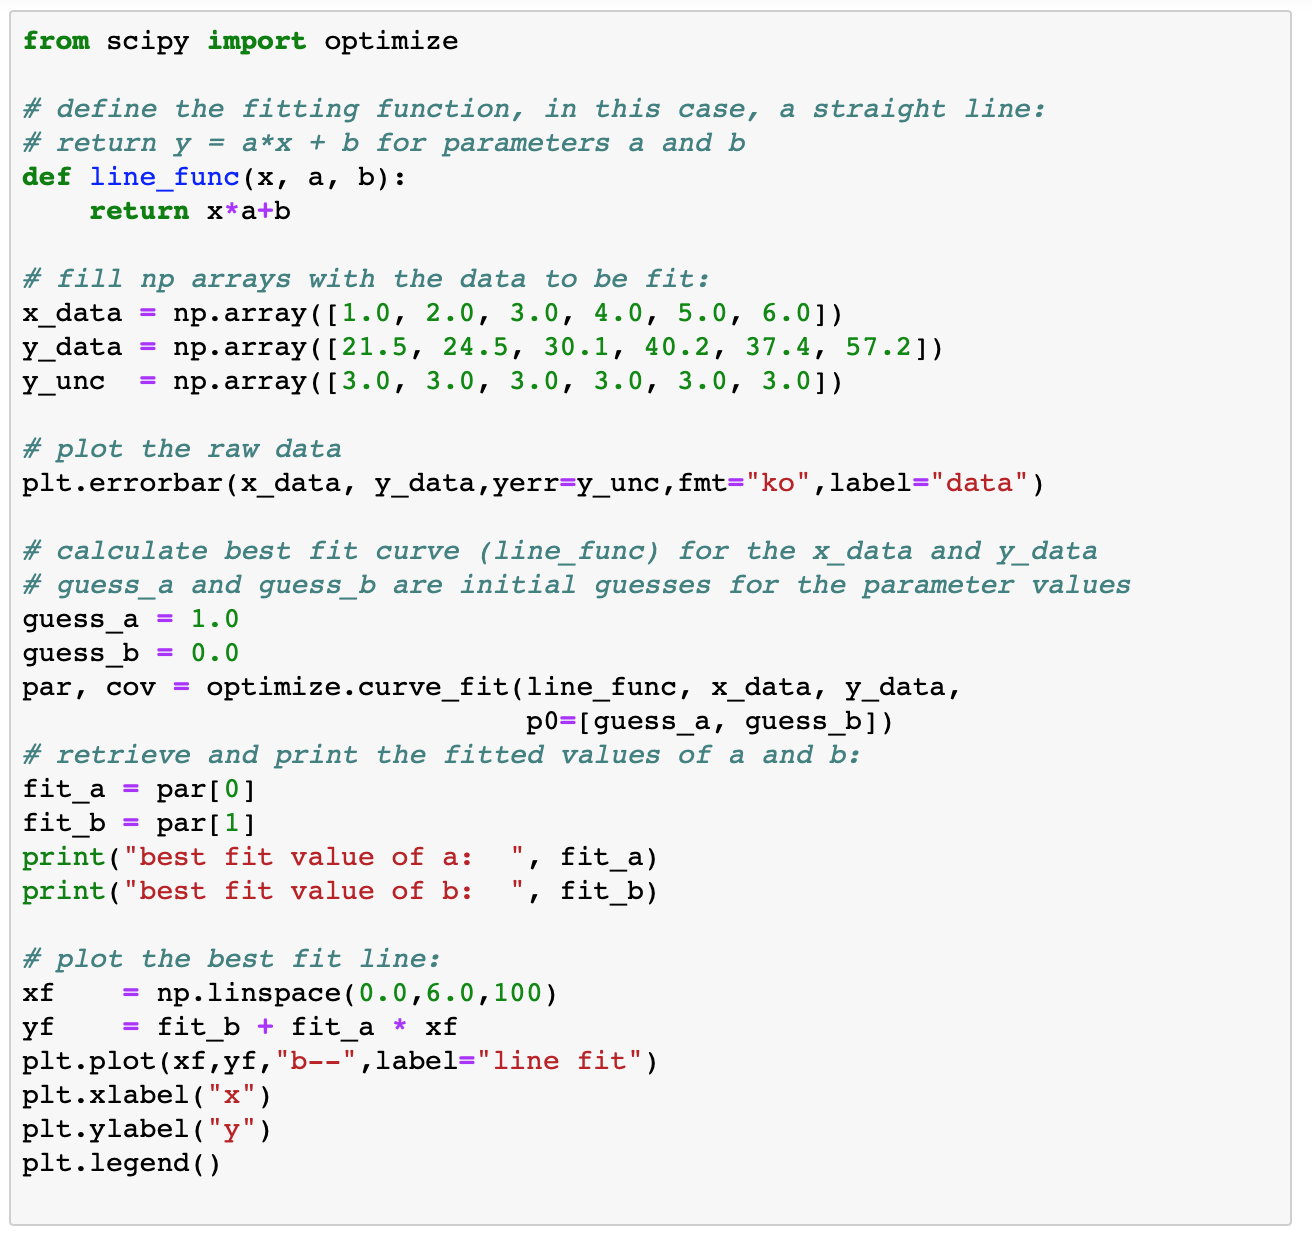
\includegraphics[width=0.65\textwidth]{figs/labs/fitting/fit_code.png} \\
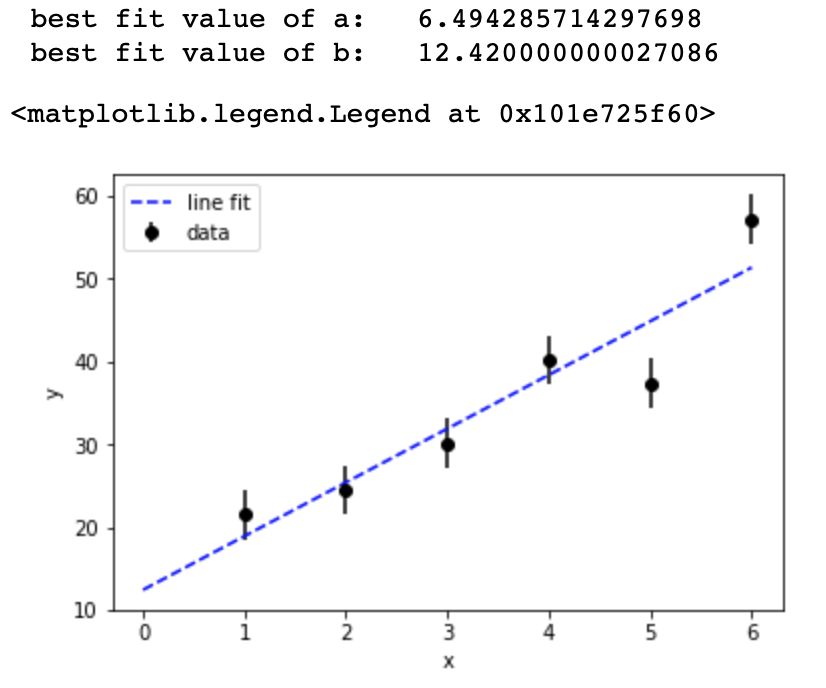
\includegraphics[width=0.65\textwidth]{figs/labs/fitting/fit_out.png} \\
\caption{Example fitting data to straight line.}
\label{fig:fiteg}
\end{center}
\end{figure}

An example using Scientific Pythons {\tt curve{\_}fit} function to fit
a straight line to data is shown in Fig.~\ref{fig:fiteg}.  A block of 
code defining the function we wish to fit, in this case, a straight
line, is defined as a function:
\begin{verbatim}
     def line_func(x, a, b):
         return a*x + b
\end{verbatim}
In this case, the function requires three parameters (in the computer
science sense) the x data in a numpy array as function parameter x,
the slope as function parameter a, and the intercept as function
parameter b.  When called, the function returns the x data multiplied
by the value a, with the value b added.  We don't directly call this
function, but in principle, it could be called like:
\begin{verbatim}
    y_data = line_func(x_data, 2.0, 0.0)
\end{verbatim}
to create a numpy array {\tt y{\_}data} constructed from {\tt
  x{\_}data} with slope 2 and intercept 0.

The next section filling numpy arrays containing the data, and
plotting it with error bars should be familiar by now.  The fit itself
is performed by the line:
\begin{verbatim}
par, cov = optimize.curve_fit(line_func, x_data, y_data, p0=[guess_a, guess_b])
\end{verbatim}
This performs a fit of the function {\tt line{\_}func} defined above
to the $x$ and $y$ data contained in the arrays {\tt x{\_}data} and
{\tt y{\_}data}.  Numerical fits generally find the local minimum,
which is not necessarily the global minimum of interest.  It is
important therefore, especially for complicated fits, to provide an
initial guess near the expected fit values.  These are provided to the
optional, named, function parameter {\tt p0}, which is set to the
python list {\tt [guess{\_}a, guess{\_}b]} which contains our initial guesses for
the fit parameters $a$ and $b$.  The function performs a least-squares
fit to find the best values of $a$ and $b$ which are returned as the
numpy array {\tt par}.  The function also returns the covariance
matrix as the numpy array {\tt cov}.

The remaining code simply uses the best fit values to plot the fitted
function as a dashed line.  Numerical fits are fickle.  Even if you
are only interested in the fitted value, you should always plot the
best-fit function and compare the results to your data as in important
check for your work.

\begin{table}
\caption{Sample data for straight line fit.}
\label{tbl:linesamp}
\begin{center}
\begin{tabular}{ll}
$x$ & $y \pm \sigma_y$ \\
1.0  & $15.9 \pm 3.0$ \\
2.0  & $23.6 \pm 3.0$ \\
3.0  & $33.9 \pm 3.0$ \\
4.0  & $39.7 \pm 3.0$ \\
5.0  & $45.0 \pm 10.0$ \\
6.0  & $32.4 \pm 20.0$ \\
\end{tabular}
\end{center}
\end{table}

%\begin{figure}[htbp]
%\begin{center}
%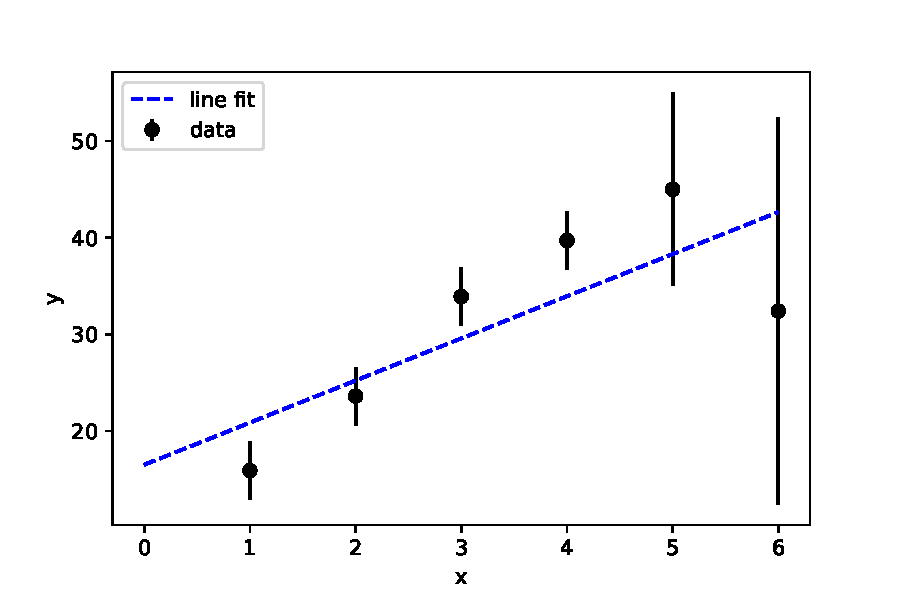
\includegraphics[width=0.65\textwidth]{figs/labs/fitting/bias.pdf} 
%\caption{This linear fit is biased by the failure to properly account for uncertainties.}
%\label{fig:fitbias}
%\end{center}
%\end{figure}

\begin{plot} Apply a code like that of Fig.~\ref{fig:fiteg}
to the data in Table~\ref{tbl:linesamp}. Plot the data including error bars and the best-fit function.
% reproduce the plot in Fig.~\ref{fig:fitbias}.  
\end{plot}

Notice that the last two data points have larger uncertainties than
the other data points.  However, the call to the {curve{\_}fit}
function does not provide the parameter uncertainties, and so the
function assumes that they all have the value $1$.  In this case,
since the uncertainties are not in fact all the same, the function
does not find the correct minimum.  The answer is clearly biased
toward the poorly measured points, because the function gives these
points the same weight as all of the other points.

\begin{print} The {\tt curve{\_}fit} function does not provide directly the $\chi^2$ value of the fit. However you can calculate it manually via equation~\ref{eqn:chi2}. The sum can be obtained via numpy function sum. Modify your code to include calculation of the $\chi^2$ value of the fit. Include also the calculation of the $\chi^2$ divided by the number of degrees of freedom (number of data points minus number of parameters), which is called reduced $\chi^2$. Print both of those values. Is the fit reasonable based on the reduced $\chi^2$ value? Print your comment as well. 
\end{print}

\begin{plot} Look-up the {\tt curve{\_}fit} function and the optional parameter
{\tt sigma}. Provide the correct uncertainties to
the fit and make a new plot with the data and the fit.  You should observe that the fit results is no longer biased,
and more closely tracks the well constrained left side of the plot. \end{plot}

\begin{print} Print $\chi^2$ and reduced $\chi^2$ value. Is the fit reasonable based on the reduced $\chi^2$ value? Print your comment as well. \end{print}

\section{Parameter Uncertainties I}
\label{sec:sigmatrue}
As discussed in the lecture the uncertainty $\sigma_{p_i}$ on the $i$th parameter $p_i$
can be determined from the second derivative of the $\chi^2$ function:
\begin{displaymath}
\frac{d^2\chi^2}{d p_i^2} = \frac{2}{\sigma_{p_i}^2}.
\end{displaymath}
In general, for $M$ parameters, the $M \times M$ covariance matrix is calculated as:
\begin{displaymath}
C(i,j) = 2 \cdot \left(\dfrac{d^2\chi^2}{d p_i d p_j} \right)^{-1}
\end{displaymath}
from which we can see that the diagonals are simply the parameter uncertainties squared:
\begin{displaymath}
C(i,i) = 2 \cdot \left(\dfrac{d^2\chi^2}{d p_i^2} \right)^{-1} = \sigma^2_{p_i}.
\end{displaymath}
The off-diagonal elements contain information about how parameters are
correlated, and for a well designed fit function they should be close to
zero.

The {\tt curve{\_}fit} function returns both the best fit parameter values and the covariance matrix:
\begin{verbatim}
par, cov = optimize.curve_fit(...)
\end{verbatim}
For a fit with $M$ parameters, we can obtain an array containing the
$M$ parameter uncertainties from the square root of the diagonals of the $M \times M$
covariance matrix:
\begin{verbatim}
unc = np.sqrt(np.diag(cov))
\end{verbatim}

We can obtain uncertainties of parameters by accessing elements of the array.

Lets study this in an example for $N=1$ parameter. Generate $x$-values as a numpy array of evenly spaced values from 0 to 99. Generate $y$-values as 100 random numbers drawn from a Gaussian distribution with mean $m = 50$ and a width $\sigma_y =10$.  Perform a fit using {\tt curve{\_}fit} function. Set the uncertainties on the $y$ values to 10 and also set parameter {\tt absolute{\_}sigma = True}.  

 The best fit constant value we expect is simply the mean of the $y$-values.  The
uncertainty on the mean value should be:
\begin{displaymath}
\sigma_m = \sigma_y / \sqrt{N} = 10 / \sqrt{100} = 1.0
\end{displaymath}

\begin{print} Calculate the expected values for the best fit value and its uncertainty. Print them together with the fitted best fit value and its uncertainty. Do those agree? \end{print}


\section{Fitting a Sine Curve}

In this section, you will fit the sample data to a sine function:
\begin{displaymath}
 y = A \, \sin( k x). 
\end{displaymath}
Use the following sample data:\\
\begin{center}
\begin{tabular}{|ll| ll|ll|}
\hline
$x$ & $y$ & $x$ & $y$ & $x$ & $y$\\
\hline
0  & 5.3    & 4  & -9.7   & 8  & 15.7  \\
1  & 15.0   & 5  & -17.4  & 9  & 18.5  \\
2  & 19.2   & 6  & -20.5  & 10 & 8.6   \\
3  & 6.8    & 7  &  2.1   & &  \\
\hline
\end{tabular}
\end{center}
Assume the uncertainty is the same for each $y$ value: $\sigma_i = 2$.
\begin{plot} Plot the data including error bars and the best-fit
sine wave. \end{plot}

\begin{print} Print the best fit parameter
values and their uncertainties. \end{print}

Remember to set {\tt absolute{\_}sigma=True}.\\

This is a \textbf{sign-off point} for this lab. 

\section{Parameter Uncertainties II}

%\begin{figure}[htbp]
%\begin{center}
%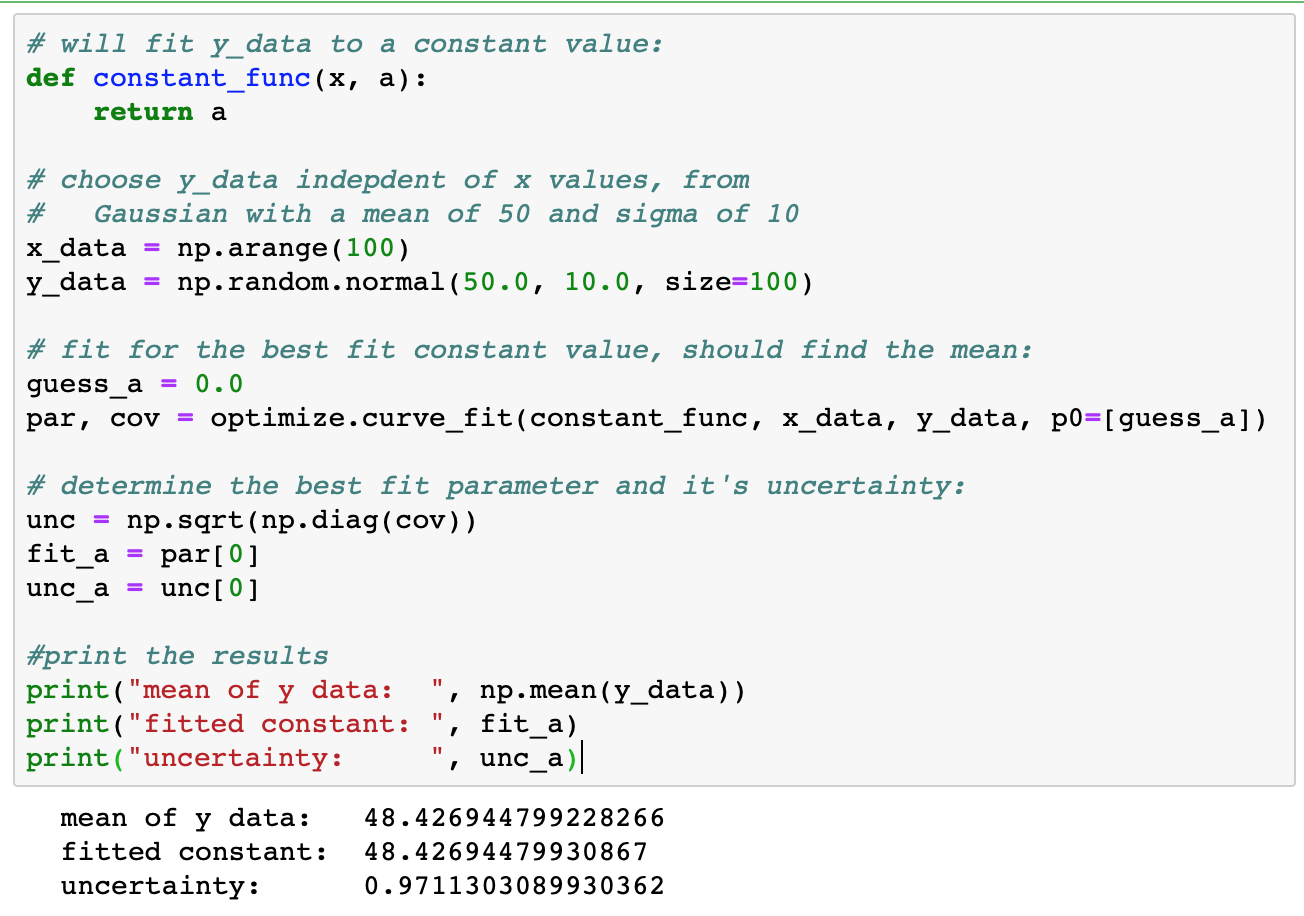
\includegraphics[width=0.65\textwidth]{figs/labs/fitting/uncertainties.png} \\
%\caption{Example obtaining parameter uncertainties.}
%\label{fig:fitunc}
%\end{center}
%\end{figure}

Lets repeat the study in~\ref{sec:sigmatrue}. Generate $x$-values as a numpy array of evenly spaced values from 0 to 99. Generate $y$-values as 100 random numbers drawn from a Gaussian distribution with mean $m = 50$ and a width $\sigma_y =10$.  Perform a fit using {\tt curve{\_}fit} function.  Leave the uncertainties on the $y$ values
unspecified and also leave parameter {\tt absolute{\_}sigma} unspecified. 

\begin{print} Print the fitted best fit value and its uncertainty. \end{print}

It's surprising actually, that the fit returns the correct
uncertainty.  Your code does not provide  the uncertainty on the $y$ parameters $\sigma_y$ to
the fit.  So how can it possible deduce the correct uncertainty
$\sigma_m = \sigma_y / \sqrt{N}$?

The answer is that behind the scenes, the {\tt curve{\_}fit} function
is being really quite clever (too clever, in my opinion, for a default
behavior!)  By default, the covariance matrix returned by the 
{\tt curve{\_}fit} function is scaled by the factor:
\begin{displaymath}
\alpha = \frac{\chi^2_{\rm min}}{\rm NDF}
\end{displaymath}
the minimum value of the $\chi^2$ divided by the number of degrees of
freedom (number of data points minus number of parameters).  As discussed in lecture that $\alpha$ is around 1 for a least-squares fit with
an appropriate model and correct uncertainties.  So nominally this
factor is one, and has no effect.  But consider what happens if the
actual uncertainties are $\sigma$ while the $\chi^2$ used in the fit assumes they
are, for example, ``1''.  In this case, the calculated $\chi^2$ is:
\begin{displaymath}
\chi^2 = \sum_i \frac{(f(x_i;p) - y_i) ^2}{1}
\end{displaymath}
which differs from the correct $\chi^2$:
\begin{displaymath}
\chi^2 = \sum_i \frac{(f(x_i;p) - y_i) ^2}{\sigma^2}
\end{displaymath}
by a factor of $\sigma^2$.  This means that while the correct value
for $\alpha$ is nearly one, the calculated value of alpha will be
$\sigma^2$.  This is precisely the factor needed to scale the squared
parameter uncertainties to account for the fact that the initial
uncertainty was $\sigma$ but we assumed $1$.

This behavior is controlled by the parameter {\tt absolute{\_}sigma}.
By default, the function sets {\tt absolute{\_}sigma = False} and
scales the covariance matrix as just described.  On the other hand, if
you want to simply use the provided uncertainties without re-scaling
the covariance matrix, you must remember to set {\tt
  absolute{\_}sigma = True}.  I think this is a really poor choice of
default behavior...  it's really quite a fancy thing to do implicitly.
In cases when you know the uncertainty on your data points, this
re-scaling actually results in less correct estimate for the
uncertainties.  This is because for a good model with proper
uncertainties, the factor $\alpha$ is near one, but not exactly one.

\begin{print} Repeat the study but leave the uncertainties on the $y$ values
unspecified and set {\tt absolute{\_}sigma = True} in the fit.  You
should obtain an uncertainty of $0.1$.  Print your value and print your explanation of
why you obtained this value. \end{print}

As a rule of thumb, when using {\tt curve{\_}fit}, if you provide
explicit uncertainties, you should remember to set {\tt
  absolute{\_}sigma = True}.  And really, for precision work, you should
almost always be providing explicit uncertainties.




















\chapter{Measurement of Planck's Constant}

\section{Introduction}

In this lab, we will measure Planck's constant by measuring the
$V$-$I$ curves of three different colored light emitting diodes
(LEDs).  An LED is a particular type of diode for which the
recombination of electrons and holes produces photons, typically in
the visible light spectrum.  These diodes have an activation voltage given by:
\begin{equation} \label{eqn:va}
V_{\rm A} = \phi + \frac{hc}{e}\frac{1}{\lambda}
\end{equation}
where $\lambda$ is the wave-length of the light produced by the diode,
and $\phi$ is the contribution to the voltage drop due to other
effects in the $p-n$ junctions.  The diodes we are using have been
chosen to ensure that $\phi$ is approximately constant across all
three diodes.

The quantity
\begin{displaymath}
\frac{hc}{e}
\end{displaymath}
can therefore be determine from the slope of the activation voltage as a function of $1/\lambda$.

The 2018 redefinition of the SI is means that the quantity
\begin{displaymath}
hc = 1.23984193~\rm eV \mu m
\end{displaymath}
is technically now exactly known, because the values $h$, $c$, and $e$
are now taken as exact values which define the corresponding SI
units. Of course, it is still useful and fun to measure this quantity
ourselves in the lab.  Since we will also be measuring the speed of
light, we'll interpret this measurement as our determination of
Planck's constant.

\section{LED Model}

For the purpose of this experiment, we will model the LED as an ideal
diode with voltage drop equal to the activation voltage $V_{\rm A}$ of
Equation~\ref{eqn:va} plus a series resistance $R_{\rm LED}$.  As
shown in Fig.~\ref{fig:ledmodel}, the effect of this resistance is to
replace the vertical line at the activation voltage $V_A$ with a line
of slope $1/R_{\rm LED}$.

\begin{figure}[htbp]
\begin{center}
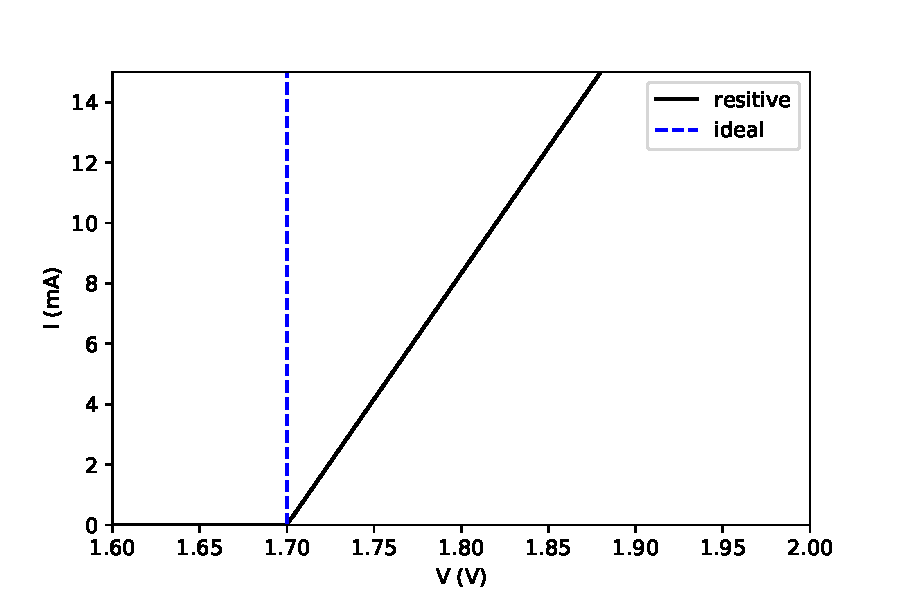
\includegraphics[height=0.3\textheight]{figs/labs/planck/model.pdf} \\
\end{center}
\caption{The LED model for $V_A=1.7~\rm V$ and $R_{\rm LED}=12~\Omega$}
\label{fig:ledmodel}
\end{figure}



\section{$V-I$ Curve from LED.}

\begin{figure}[htbp]
\begin{center}
\begin{circuitikz}[line width=1pt]
\draw (0,0) to[voltage source,bipoles/length=1.5cm,l=$V_1$] ++(0,4.0) to[short] ++(2.0,0) coordinate(C);
\draw (C) to[R, l_=$R_1$] ++(0,-2.0) coordinate(B) to[empty diode, l_=LED] ++(0,-2.0) coordinate(A) to[short] ++(-2.0,0.0);
\draw (A) to[short,*-] ++(1.5,0) to[short] ++(0,0.8) node[component]{V} to[short] ++(0,0.8) to[short,-*] ++(-1.5,0);
\draw (C) to[short,*-] ++(1.5,0) to[short] ++(0,-0.8) node[component]{V} to[short] ++(0,-0.8) to[short,-*] ++(-1.5,0);
\end{circuitikz} 
\end{center}
\caption{experimental setup.}
\label{fig:planck_setup}
\end{figure}

Construct the experimental setup shown in Fig.~\ref{fig:planck_setup}
using a $1~\rm k\Omega$ precision $1\%$ resistor for $R_1$, a green
LED (see Table~\ref{tbl:led}) , and using your bench-top DC supply to provide $V_1$, initially
set to $0~\rm V$.  Connect Mastech voltmeter across the resistor $R_1$ and
Triplett voltmeter across the LED.  When constructing your circuit,
make sure the LED can be easily removed and replaced.  Also keep in
mind that the longer lead is the positive terminal of the LED, i.e.,
the upper terminal of the LED as drawn in the
Fig.~\ref{fig:planck_setup}.  Set both voltmeters to the $20~\rm V$
setting.

Test your circuit first by turning up the voltage on your supply to
about $5~\rm V$ and checking that the LED lights up.  The voltmeter
across the resistor $R_1=1~\rm k\Omega$ is effectively measuring the
current in $mA$ as $1~{\rm V}/1~{\rm k\Omega} = 1~\rm mA$.  Do not
misunderstand this statement to mean you should set the multi-meter to
the current measurement: we measure the voltage, but from $Ohm's Law$
we know the current in resistor.  The voltmeter across the diode is
measuring the diode drop $V_{\rm D}$.

$I = 0.5,1.0,2.0,4.0,6.0,8.0,10.0,12.0~\rm mA$ are target values for your current. 
Take a series of measurements of $V_{R_1}$ and $V_D$ near target values of $I$
by adjusting the voltage provided by your DC supply until the current $I$, as derived from measured
voltage across $R_1$, is near the target value.  Remember
not to waste time fussing to make the measurement at exactly the
target value.  For instance, measuring at $I=2.16~\rm mA$ instead of
the target $I=2.0 ~\rm mA$ is perfectly acceptable.  
\begin{measurement} Record a sketch of your setup in the logbook. 
\end{measurement}
\begin{measurement} 
Record in your logbook the measured values of $V_{\rm R_1}$, the accuracy $\Delta V_{\rm R_1}$, $I$ derived from $V_{\rm R_1}$, uncertainty $\Delta I$, measured values of  $V_{\rm D}$ and the accuracy $\Delta V_{\rm D}$. In addition record the fractional uncertainty of $I$ and $V_{\rm D}$. See table~\ref{tbl:example} for example on how to log the data. See table~\ref{tbl:accuracy} for accuracy of the multimeters. You  can neglect uncertainty on $R_1$ value when calculating uncertainty of $I$.
\end{measurement}
 

\begin{table}
\begin{center}
\caption{Example of table to record data.
\label{tbl:example}
%Instructor data from a red LED not used
}
%\begin{tabular}{lll}
%target $I$ (mA) & $I$ (mA) & $V_{\rm D}$ (V) \\
%\hline
%0.5  &  0.44  & 1.62 \\
%1.0  &  0.95  & 1.66 \\
%2.0  &  1.99  & 1.71 \\
%4.0  &  4.15  & 1.77 \\
%6.0  &  6.05  & 1.81 \\
%8.0  &  8.09  & 1.85 \\
%10.0 &  10.04 & 1.88 \\
%12.0 &  12.02 & 1.91 \\ 
%\end{tabular}
\begin{tabular}{llllllllll}
target $I$ (mA) & $V_{\rm R_1}$ (V) & $\Delta V_{\rm R_1}$ & $I$ (mA) & $\Delta I$ & \% $I$ &$V_{\rm D}$ (V) & $\Delta V_{\rm D}$ (V) & \% $V_{\rm D}$ \\
\hline
0.5 & \dots &  \dots &  \dots & \dots  & \dots & \dots & \dots & \dots  \\
\end{tabular}
\end{center}
\end{table}

\begin{measurement} 
Repeat this measurement using a yellow LED (see Table~\ref{tbl:led}).
\end{measurement}

\begin{measurement} 
Repeat this measurement using a red LED (see Table~\ref{tbl:led}).
\end{measurement}


\begin{table}[htbp]
\begin{center}
\caption{LEDs used in this experiment.}
\label{tbl:led}
\begin{tabular}{llll}
color & part no. & $\lambda$ (nm) & max current \\
%blue  & WP710A10QBC & 460 & 30 mA \\
green & WP710A10GT & 565 & 25 mA \\  
yellow & TLHY4405 & 581-594 & 30 mA \\ 
red & TLHR4405 & 612-625 & 30 mA \\ 
\end{tabular}
\end{center}
\end{table}

\section{Analysis}

\begin{figure}[htbp]
\begin{center}
\begin{tabular}{cc}
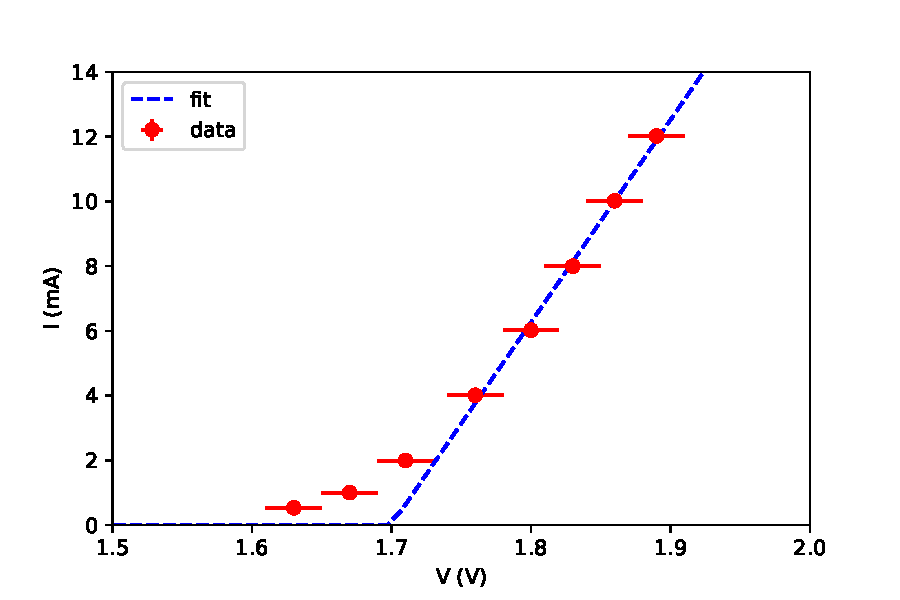
\includegraphics[width=0.45\textwidth]{figs/labs/planck/fit_diode.pdf} &
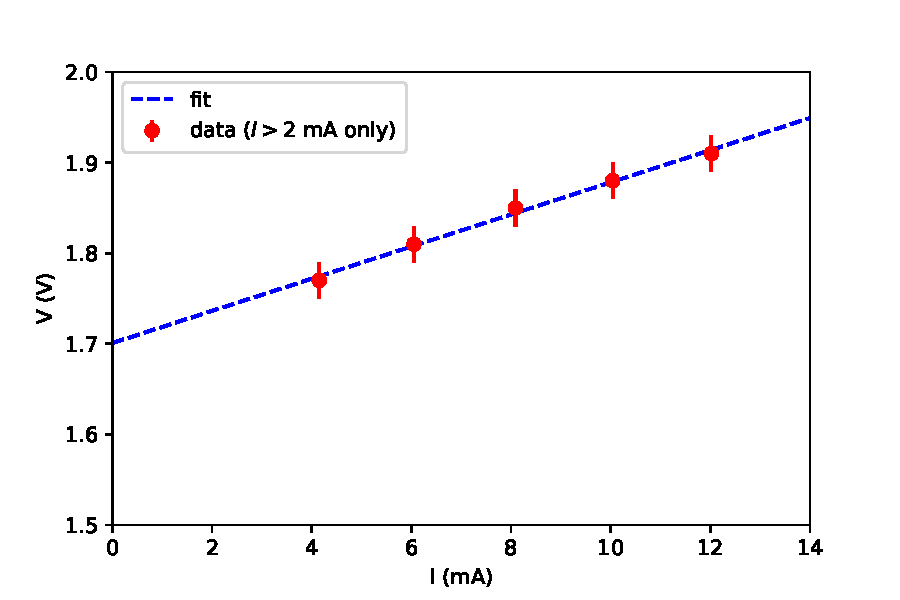
\includegraphics[width=0.45\textwidth]{figs/labs/planck/fit_vi.pdf} \\
(a) & (b) \\
\end{tabular}
\end{center}
\caption{Example fit for red LED.  The (a) real diode response
  departs from the simple linear model for $I \leq 2~\rm mA$, so the
  (b) fit for the linear response is performed for $I > 2~\rm mA$.
  Note that $V_{\rm D}$ is taken as the $y$-axis for the purpose of fit,
  because the voltage uncertainties are the dominant uncertainty in
  the fit.  Notice also that the $0.02~\rm V$ uncertainty reported by
  the DMM specifications appears to be predominantly systematic.}
\label{fig:redfit}
\end{figure}

The example of the V-I response for a red diode is
plotted in Fig~\ref{fig:redfit}a.  Notice that at large values for the
current ($I > 2~\rm mA$) the V-I response is linear, indicating that it
is dominated by internal resistance of the diode.  As lower current
($I \leq 2~\rm mA$) the V-I response is exponential, as expected for a
real diode.  We will fit our simple linear model for the diode
response only in the region where this approximation is valid, for
$I>2~\rm mA$. 

As shown in Fig.~\ref{fig:redfit}b, perform a linear
fit only for the data with $I>2~\rm mA$.

%With the DMM set to the $20~\rm V$ scale, the uncertainty on your
%measured values for $V$ and $I$ is approximately $0.02~\rm V$ and
%$0.02~\rm mA$ respectively.  



\begin{measurement} 
Because the measured voltage range is
less than a volt, but the measured current range is around $10~\rm
mA$, it is the uncertainties on the voltage that dominate the
uncertainty on both the slope and intercept of the linear function in our fit range. Show this is true for your measurement by looking at the percent uncertainties of $I$ and $V_{\rm D}$ that you recorded in your logbook. Record your observation in the logbook.
\end{measurement}


We therefore choose to use $V$ as the $y$-axis and and $I$ as the
$x$-axis for the purposes of fitting, because the $\chi^2$ analysis of
the {\rm curve{\_}fit} function only considers uncertainties in the
$y$-axis.  There are straightforward ways to handle uncertainties in
both $x$ and $y$, but they add complexity which is best avoided if
possible.

\begin{plot} For red LED data, fit the $V$ versus $I$ data to a linear function, and
determine the best fit resistance and activation voltage, and the
uncertainties.  
%Assume the uncertainty on the measured voltages is $0.02~\rm V$ for each data point 
Use uncertainties on the measured voltages
and only consider $I > 2~\rm mA$ in
the fit.  Remember to set {\tt absolute(\_)sigma=True} in your fit so
that the fit uncertainties are based on the absolute uncertainties
without re-scaling. \end{plot}

\begin{plot} 
Repeat this analysis for yellow LED data.
\end{plot}

\begin{plot} 
Repeat this analysis for green LED data.
\end{plot}

\begin{figure}[htbp]
\begin{center}
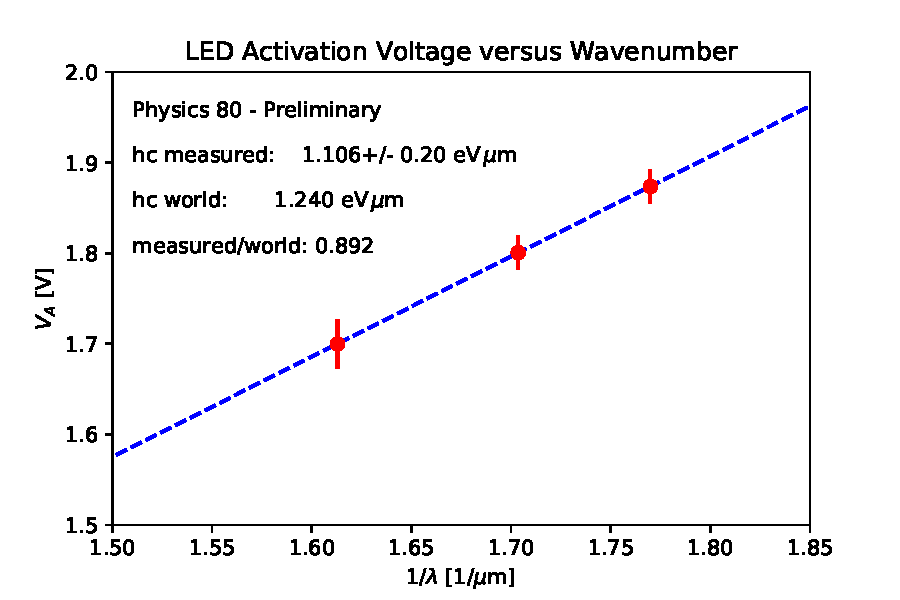
\includegraphics[height=0.3\textheight]{figs/labs/planck/planck.pdf} \\
\end{center}
\caption{Example plot for determination of $hc$.}
\label{fig:planckfit}
\end{figure}

\begin{plot} 
Plot the best-fit $V_A$ of each diode versus $1/\lambda$, and
determine the slope ($hc/e$) and its uncertainty from a linear
fit.  The example plot is shown in Fig.~\ref{fig:planckfit}.
Recall that $1~\rm eV$ is the change in potential energy of one
electron passing through $1~\rm V$ of potential energy, allowing you
to conveniently convert the slope in $\rm V \mu m$ to $\rm eV \mu m$ for
comparison with the established value $hc = 1.240~\rm eV \mu m$.
\end{plot}
\begin{print}
Does your measured value of  $hc$ agree with the known value? Print how many  sigma values your  measured value lies with respect to the known value, as well as your brief comment on this.
\end{print}


\section{Systematic Uncertainties}

In addition to the statistical uncertainties reported by the fit,
their are a number of systematic uncertainties.  For this lab, we'll
consider one obvious source of systematic uncertainty, which arises
from our treatment of the real diode response as a simple linear
function.

To determine the size of this systematic uncertainty, we measure the
effect of this assumption on our measured valued.  One simple way to
estimate this effect is to remove the requirement $I>2~\rm mA$ from
our analysis.  The difference between the measured value for $hc$ as
determined with and without the cut on $I>2~\rm mA$ can be interpreted
as a systematic uncertainty due to our simplistic model.

\begin{print} Repeat your analysis without the requirement $I > 2~\rm mA$ and take
this as the overall systematic uncertainty on your measurement. Print your result in the following form 
\begin{displaymath}
 \textbf{hc}= \textit{your value here} \pm \textit{your value here} \,  ({\rm stat}) \pm\textit{ your value here} \, ({\rm syst})
\end{displaymath}
\end{print}

\noindent
This is a \textbf{sign-off point} for this lab. 













\documentclass[12pt,oneside]{book}

\usepackage[dvips,letterpaper,margin=0.75in,bottom=0.75in]{geometry}
\usepackage{cite}
\usepackage{slashed}
\usepackage{graphicx}
\usepackage{amsmath}
\usepackage{enumitem}

\usepackage[american,fulldiode]{circuitikz}
\tikzset{component/.style={draw,thick,circle,fill=white,minimum size =0.75cm,inner sep=0pt}}

\begin{document}
\ctikzset{bipoles/thickness=1}
\ctikzset{bipoles/length=.6cm}

\title{Physics 80 Lab Manual}

\maketitle

\chapter{The Speed of Light in Air }

\section{Pre-lab Calculations}
\noindent
1) Suppose .  Hint: assume a . \\ 

\noindent
2)   \\

\noindent
3) What is the definition of the meter ? What is the exact value of the speed of light in vacuum?
%The meter  is the length of the path travelled by light in vacuum during a time interval of 1/299792458 second. The exact value for the speed of light in vacuum is 299,792,458 metres per second.

\section{Introduction}

In this lab, you will measure the speed of light in the air by measuring the time between sending and receiving a flash of light over a known distance, evaluate statistical and systematic uncertainties and compare it to the known value.  In the process, you will learn how to use your scope to make time measurement.

The flash of red light is created by a pulsed laser diode, a device very similar to a laser pointer, except this laser is switched on and off (pulsed) at a very high rate: 1 million times per second (1 MHz).  Whenever laser diode is pulsed a "trigger" pulse is sent to the oscilloscope. The pulsed beam of light is detected by a fast photo-diode detector and a "signal" pulse is sent to the oscilloscope. The time difference between the two pulses $\Delta t$ can be measured as a function of the distance $L$ between the laser/detector apparatus. 
Assuming that the time difference between the two pulses depends only on the time it took the light to travel the distance $L$ one can determine the  phase velocity of laser diode light in the air:   $v_{red}=\frac{L}{\Delta t}$.


%and the
%mirror
%can be bounced off of
%a mirror and the return pulses detected by a very responsive (“fast”) detector. Each pulse of the laser
%creates two signals, one from the laser itself (the “trigger”) and one from the detector when it picks up the
%returning pulse. These two signals can be compared to each other with a fast oscilloscope, and the time
%between them can be measured as a function of the distance between the laser/detector apparatus and the
%mirror. By varying the total distance from the laser to the detector L and monitoring the time difference
% on the scope, one can determine the speed of light c. If the time difference between the two signals 
%depended only on the time it took for the light to travel that distance, then c would be given by


\section{Measuring the $I$-$V$ Curve of a Diode}

In this section you will measure the $I$-$V$ curve of a 1N914 diode, and compare your results to the curves available from the device data sheet.  To avoid taking a bunch of measurements by hand, we will use a trick to plot the curve directly on your oscilloscope using the XY mode.
\begin{figure}[htbp]
\begin{center}
\begin{tabular}{c@{\hskip 2cm}c}

\begin{circuitikz}[line width=1pt]
\draw
(0,0) to[sinusoidal voltage source,bipoles/length=1.5cm,l=$\tilde{V}$] (0,4) -- (2,4);
\draw
(2,4) node[right]{$P_2$} to[resistor,l=$R_1$,o-o] (2,2) node[right] {$P_1$} to[diode,l=$D_1$,-o](2,0) node[right]{G}-- (0,0)
;
\draw (0,0) -- ++(0,0) node[ground,yscale=2.0]{};
\end{circuitikz} &

\begin{circuitikz}[line width=1pt]
\draw
(0,0) to[sinusoidal voltage source,bipoles/length=1.5cm,l=$\tilde{V}$] (0,4) -- (4,4);
\draw
(2,4) to[resistor,l_=$R_1$,*-o] (2,2) node[left]{$P_1$} node[right]{(Ch.1)} to[diode,l_=$D_1$,o-*] (2,0)
(4,4) to[diode,l=$D_2$,-o] (4,2) node[right] {$P_2$ (Ch.2)} to[resistor,l=$R_2$,-o](4,0) node[right]{G}-- (0,0)
;
\draw (2,0) -- ++(0,0) node[ground,yscale=2.0]{};
\end{circuitikz} \\
(a) & (b) \\
\end{tabular}
\caption{Diode circuits for (a) demonstrating rectification and (b) plotting the diode IV curve on your oscilloscope.}
\label{fig:diodecircuits}
\end{center}
\end{figure}

Consider (but don't build!) the circuit in Fig.~\ref{fig:diodecircuits}a.  The voltage between points $P_2$ and $P_1$ is proportional to the current passing through the diode, and the voltage between points $P_1$ and $G$ is the voltage across the diode.  So if we could display $P_2-P_1$ versus $P_1-G$ on your scope we could use this circuit.  Unfortunately, this is not possible on your scope, because (1) the only valid place to put the scope probe ground shield clips is at the point $G$ (Why?) and (2) you can only display Channel 1 versus Channel 2 in XY mode.   

The solution is to drive two copies of the diode in series resistor, with the component order reversed, as in Fig.~\ref{fig:diodecircuits}b.  This way, we can connect the probe ground shields as required at point $G$, put the voltage across the diode on scope Channel 1 by connecting the probe tip at $P_1$, and put the voltage across the resistor (proportional to current through the diode) on scope Channel 2 by connecting the probe tip at $P_2$.

Build the circuit in Fig.~\ref{fig:diodecircuits}b using a 1N914 fast switching diode for $D_1$ and $D_2$ and $R_1= R_2 = 10~{\rm k\Omega}$.  Set your function generator for high-impedance output, providing AC with peak to peak voltage of $20~\rm V$ at a frequency of $100~\rm Hz$.  Before switching to XY mode, make certain that your Channel 1 has no voltage offset (that is, zero voltage is located at the origin) or else your diode output voltage won't be calibrated properly in your output plot.   Once you set this, try not to adjust the offset of Channel 1 or you'll have to redo it!  To minimize noise, set the bandwidth limit ``On'' for both channels (this is available in the menu for each input channel as ``BW Limit'').

\begin{figure}[htbp]
\begin{center}
\begin{tabular}{c@{\hskip 2cm}c}
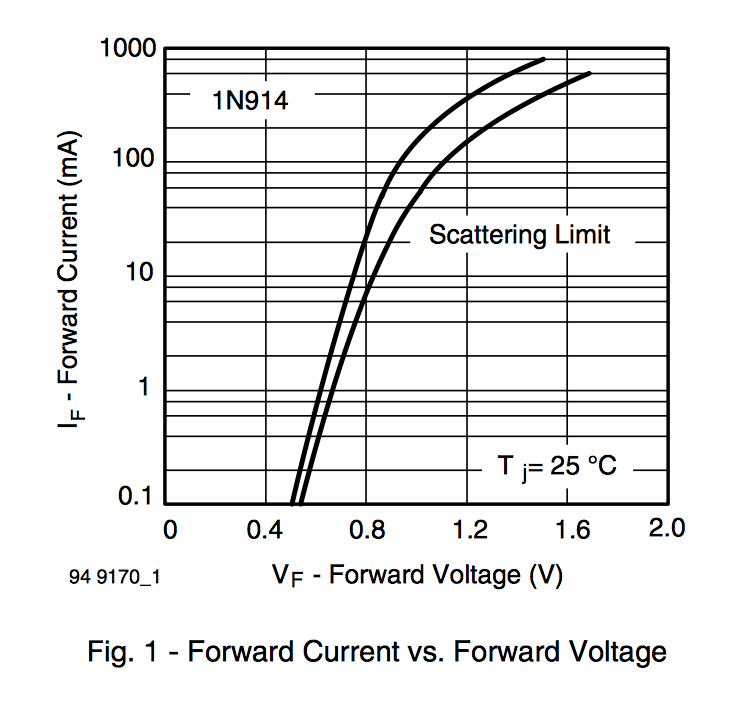
\includegraphics[height=0.25\textheight]{figs/labs/diode/1N914.png} &
\begin{picture}(200,100)
\put(0,0){\includegraphics[height=0.25\textheight]{figs/labs/diode/diodeiv.png}}
\put(10,52){$0~mA$}
\put(10,70){$0.2~mA$}
\put(10,88){$0.4~mA$}
\put(10,106){$0.6~mA$}
\put(10,124){$0.8~mA$}
\put(10,142){$1.0~mA$}
\end{picture}\\
(a) & (b) \\
\end{tabular}
\caption{\label{fig:diodeiv} IV curves for the1N914 from (a) data sheet, and (b) as you will measure in this lab.  In the scope trace, the Channel 2 ($Y$) with scale set to $2~\rm V$ measures the voltage across a $10~\rm k\Omega$ resistor, so each division corresponds to $200~\rm \mu A$ as indicated. 
}
\end{center}
\end{figure}

Set the scope into XY mode, and see if you can reproduce the diode IV curve in Fig~\ref{fig:diodeiv}b.
Beats jotting down voltages in your logbook doesn't it?  Now jot down the voltage you expect across the diode for a current of $1~\rm mA$ in your logbook.  Where they overlap, does your measured IV curve agree with the curve from the component data sheet in Fig.~\ref{fig:diodeiv}a?

\section{Rectifying an AC Signal}

\begin{figure}[htbp]
\begin{center}
\begin{circuitikz}[line width=1pt]
\draw
(0,0) to[sinusoidal voltage source,bipoles/length=1.5cm,l=$\tilde{V}$] (0,4) -- (2,4)
(2,4) node[right]{$P_2$} to[diode,l=$D$,o-o] (2,2) node[right] {$P_1$} to[resistor,l=$R$,-o](2,0) node[right]{$G$} -- (0,0)
(2,0) -- ++(0,0) node[ground,yscale=2.0]{};
\end{circuitikz} 
\caption{A diode rectification circuit.}
\label{fig:rect}
\end{center}
\end{figure}

Set your function generator to provide an AC source with frequency $100~\rm Hz$ and peak-to-peak voltage $V_{\rm pp}=5~\rm V$.  Build the circuit in Fig.~\ref{fig:rect} using a 1N914 diode for $D$ and $R=1.8~\rm k\Omega$. 

With your scope probe ground shield clips both properly connected to the ground at $G$, monitor the voltage at points $P_1$ and $P_2$.   Sketch the voltage across the resistor $R$ and the voltage supplied by the function generator versus time on the same plot in your lab book. 

Using your scopes amplitude measurement feature, measure precisely (i.e. to within $50~\rm mV$ precision) the voltage drop across the diode at the peak current value, by measuring the difference between Channel 1 and Channel 2 of your scope at the peak.  Is this operating point consistent with your results from the previous section and the pre-lab calculations?


\section{Lab Report}

Your report should include all of your measurements and a comparison with your calculation.
 

\end{document}
\chapter{Muon Lifetime}

\section{Introduction}

\begin{figure}[htbp]
\begin{center}
{\includegraphics[width=0.35\textwidth]{figs/labs/muon/cosmic_ray.jpg}}\\
\end{center}
\caption{\label{fig:cosmic}  Cosmic ray shower induced by a primary cosmic ray (typically protons) striking an atom in the upper atmosphere.}\end{figure}

The muon is a fundamental particle in the Standard Model of particle
physics.  It is essentially a heavier version of the electron.  Like
the electron, the muon has a corresponding anti-particle, the
anti-muon ($\mu^+$).  Muons are readily available for study because
they are produced as a result of showers that are induced by incident
cosmic rays that constantly bombard the earth.  Typical primary cosmic
rays are protons, and there collisions with nuclei in the upper
atmosphere produce mainly protons, neutrons, and pions.  The
subsequent decays of these particles produce electrons, neutrinos, and
the muons we will be studying.  The flux of muons at sea-level is
about 1 per ${\rm cm}^2$ per minute, and this population has a mean
kinetic energy of about $4~\rm GeV$.  Such muons are highly
penetrating: they pass quite readily through buildings.

The muon decays via the weak interaction, its most probable decays being:
\begin{eqnarray*}
\mu^- \to e^- + \bar{\nu}_e \nu_\mu,\\
\mu^+ \to e^+ + \bar{\nu}_\mu \nu_e.
\end{eqnarray*}
As fundamental particles, muons are indistinguishable from one
another, and therefore the decay rate for a population of $N$ muons
must be simply proportional to $N$:
\begin{displaymath}
\frac{dN}{dt} = -\frac{N}{\tau}
\end{displaymath}
The solution to this differential equation is:
\begin{displaymath}
N(t) = N(0) \exp(-t/\tau).
\end{displaymath}
In this lab, you will measure the lifetime of the muon, which has the value 
\begin{displaymath}
\tau_\mu = 2.1969811(22) \mu s
\end{displaymath}
in vacuum as reported by the Particle Data Group (PDG) with the
uncertainty in parenthesis.  Interactions with the scintillator
material in this experiment lead to a slightly different expectation
for the lifetime as discussed below.

Muons are produced at a typical height $15~\rm km$ above sea-level,
and so, in the earth frame, their transit time from the upper
atmosphere to our lab is therefore about $50~\rm \mu s$ or about 20
lifetimes.  The fact that we see an appreciable number of them at sea
level, given an upper limit on their production rate in the
atmosphere, is clear evidence for time dilation.

\section{Experimental Setup}

\begin{figure}[htbp]
\begin{center}
{\includegraphics[width=0.55\textwidth]{figs/labs/muon/setup.png}}\\
\end{center}
\caption{\label{fig:setup}  Experimental setup.}\end{figure}

The active component of the particle detector used in this experiment
is a polyvinyltoluene-based plastic scintillator in the shape of a
cylinder with a $15~\rm cm$ diameter and a $12.5~\rm cm$ height.  All
materials absorb energy due to the passage of ionizing radiation.
Scintillators are materials which re-emit a fraction of this energy as
visible light, typically in the blue to near UV range.  The light
yield is relatively low, so a sensitive photomultiplier tube is used
to amplify a modest number of photons into a large easily measurable
voltage.

\begin{figure}[htbp]
\begin{center}
{\includegraphics[width=0.65\textwidth]{figs/labs/muon/cosmics_raw.pdf}}\\
\end{center}
\caption{\label{fig:cosmics_raw}  Three days of cosmic ray data, plotted as the distribution in digitized time measurement (TDC counts).}
\end{figure}


Muons are therefore constantly passing through the scintillator,
depositing energy, and causing observable PMT pulses which are
recorded by the data acquisition system (DAQ).  Occasionally, however,
a relatively low-energy muon enters the scintillator and deposits all
of it's kinetic energy, coming to rest.  As an unstable particle, it
eventually decays into a highly-energetic electron and neutrinos.  The
electron deposits additional energy in the scintillator which is
observed as a second pulse.  The time interval between two consecutive
pulses is digitized using a time-to-digital (TDC) converter, which
converts analog time interval into a digital number.  In this case, we
use a 12-bit TDC, so the measured digital values are integers in the
range from 0 to $2^{12}-1 = 4095$.  To interpret these raw TDC counts
as a time value in microseconds, you will need to calibrate the TDC as
described below.

Three days of data has already been collected for you, and is plotted
in Fig.~\ref{fig:cosmics_raw} .  This data is available on the course
web site in the file {\tt cosmics.npy} available You load this data
using the numpy {\tt load} command, taking care to handle the
directory path correctly.  As can be seen from the plot, most of the
recorded events have the maximum possible value 4095.  This is how the
DAQ records a single pulse, with no secondary pulse in the timing
window of the TDC.  This is what happens most of the time.

The remaining events, with a measured time below the maximum value, are from events were two pulses were detected within the timing window of the TDC.  This time
interval, the decay time of the muons in this population, will have a
time-dependence given by:
\begin{displaymath}
-\frac{dN}{dt} = \frac{N(0)}{\tau} \exp(-t/\tau)
\end{displaymath}
which you will use to extract the muon life time.  This is possible because the muon decay rate ($\lambda$)
and it's lifetime $\tau$ are simply recipocrals:
\begin{displaymath}
\lambda \equiv \frac{-\frac{dN}{dT}}{N(t)} = \frac{1}{\tau}.
\end{displaymath}
This exponential decay feature is clearly visible in the raw data as the downward sloping line on the right side of this semilog plot.

There is an additional source of background for two pulse events, which arises from the possibility for two muons to arrive independently within the time window of the TDC.   Sine the arrival time of the two muons is independent, this contribution is flat in time, and is clearly visible in the raw data on the left-hand side, where the exponential contribution becomes small.

\section{Calibration}

\begin{figure}[htbp]
\begin{center}
{\includegraphics[width=0.65\textwidth]{figs/labs/muon/pulser_4_raw.pdf}}\\
\end{center}
\caption{\label{fig:pulser_raw}  Calibration run with pulses spaced $4~\mu s$ apart.}
\end{figure}

To interpret the output of the TDC (digital TDC counts as integers in
the range from 0 to 4095) as physical times in units of microseconds,
a calibration is needed.  We are using a good TDC which we can assume has a linear response, meaning that the time interval and TDC counts are related as:
\begin{displaymath}
TDC = a \cdot \Delta t  + b 
\end{displaymath}

To determine the calibration parameters $a$ and $b$ we use an LED
pulser feature built into the detector.  The LED pulser feature
flashes light into the PMT in a controlled manner, so that two pulses
a distance $\delta t$ in time apart are sent repeatedly to the TDC.
An example of 1000 pulser events with $\Delta t = 4 \mu s$ is shown in
Fig.~\ref{fig:pulser_raw}.  A total of four pulser runs of 1000 events
each with $\Delta t = 1,2,4,8$ have already been collected.  The data
from these four calibration runs available on the course website with
names like {\tt pulser{\_}4.npy} for the $\Delta t = 4~\rm \mu s$ run.

{\bf Plot 1:}  for each pulser run, compute the mean value of the recorded data and an uncertainty on this mean value.
Plot these mean values, and their uncertainties, versus $Delta t$.  Fit the linear response to obtain the parameters $a$ and $b$.  Plot the best fit linear function alongside the data.

\section{Muon Lifetime Analysis}

{\rm Plot 2: } With the calibration constants $a$ and $b$ convert the
TDC counts of the recorded comsics data and plot the distribution of
times.  You should omit all events with RAW TDC count of 4095, as
these are single pulse events.  Fit the distribution to an exponential
function plus a constant value for the flat (combinatoric) background.
Plot your fit function against the recorded data.

Report the statistical uncertainty on the fitted value for
the muon lifetime.  In addition, there are several systematic
uncertainties associated with the experiment.  The largest is the
effect of material interactions on the lifetime of the muon, which is
about $5\%$.  Other systematic effects are smaller, and can be
neglected.


%\section{Muon / Anti-Muon Ratio}

%Due to additional decay processes when captured by an atomic nucleus, the decay time of the negatively %charged muon in matter is lower than its free space value:
%\begin{eqnarray*}
%\tau_- &=& 2.043(3) \times 10^{-6} \mu s \\
%\tau_+ &=& 2.1969811(22) \times 10^{-6} \mu s
%\end{eqnarray*}
%where we have used the measured values in carbon, which should be close to value for our organic %scintillator.

%As discussed in class, you can determine the ratio $\rho$ of anti-muons to muons from the relation:
%\begin{displaymath}
%\rho = - \frac{\tau_+}{\tau_-} \cdot \frac{\tau_- - \tau}{\tau_+ - \tau}
%\end{displaymath}
%where $\tau$ is the measured valued of the muon lifetime.



\end{document}

% OTHER IDEAS:
% Fourier Transforms
% Monte Carlo techniques
% Speed of Light in Cable
% Measure e from shot noise
